%CLASSE DOCUMENTO - LINGUA E DIMENSIONE FONT
\documentclass[11pt]{toptesi}

%%%%%%%%%%%%%%%%%%%%%%%%%%%%%%%%%%%%%%%%%%%%%%%%%%%%%%%%%%%%%%%

% INCLUSIONE PACCHETTI
\usepackage[utf8]{inputenc} %utf8
\usepackage[italian]{babel}
\usepackage[T1]{fontenc}
\usepackage{blindtext}
\usepackage{graphicx,wrapfig}
\usepackage{booktabs}
\usepackage{lmodern}
\usepackage{varioref}
\usepackage{url}
\usepackage{array}
\usepackage{paralist}{\obeyspaces\global\let =\space}
\usepackage{verbatim} 
\usepackage{subfig}
\usepackage{tabularx}
\usepackage{amsmath}
\usepackage{amsfonts}
\usepackage{float}
\usepackage{amssymb}
\usepackage{multicol}
\usepackage{multirow}
\usepackage{listings}
\usepackage[pass]{geometry}
\usepackage[figuresright]{rotating}
\usepackage{algorithm}
\usepackage{algorithmic}
\usepackage{amsmath}
\usepackage[babel]{csquotes}
\usepackage{hyperref}
\usepackage[backend=bibtex]{biblatex}
\usepackage{pbox}
\usepackage{longtable}
\usepackage[dvipsnames]{xcolor}
\usepackage{amsfonts}

%%%%%%%%%%%%%%%%%%%%%%%%%%%%%%%%%%%%%%%%%%%%%%%%%%%%%%%%%%%%%%%

% CONFIGURAZIONE LINK E RIFERIMENTI
\hypersetup{%
    pdfpagemode={UseOutlines},
    bookmarksopen,
    pdfstartview={FitH},
    colorlinks,
    linkcolor={black}, %COLORE DEI RIFERIMENTI AL TESTO
    citecolor={blue}, %COLORE DEI RIFERIMENTI ALLE CITAZIONI
    urlcolor={blue} %COLORI DEGLI URL
}

%%%%%%%%%%%%%%%%%%%%%%%%%%%%%%%%%%%%%%%%%%%%%%%%%%%%%%%%%%%%%%%

% CONFIGURAZIONE LISTATI/CODICE - CANCELLARE SE NON NECESSARIO
% PYTHON - BIANCO E NERO
\lstset{%
	captionpos=b,
	language=Python,
	basicstyle =\small\ttfamily,
	keywordstyle=\color{black}\bfseries,
	breaklines=true,
	breakatwhitespace=true,
	frame=lines,
	numbers=left,
	numberstyle=\footnotesize,
}

%%%%%%%%%%%%%%%%%%%%%%%%%%%%%%%%%%%%%%%%%%%%%%%%%%%%%%%%%%%%%%%

% FRENCHSPACING VA _SEMPRE_ ABILITATO PER DOCUMENTI IN ITALIANO
\frenchspacing

%%%%%%%%%%%%%%%%%%%%%%%%%%%%%%%%%%%%%%%%%%%%%%%%%%%%%%%%%%%%%%%

%DEFINIZIONE SEZIONI IN NUMERAZIONE ROMANA
%ELENCO DEI LISTATI/CODICI
\makeatletter
\newcommand\listofcodes{%
 \iffrontmatter\else\frontmattertrue\fi
 \if@openright\cleardoublepage\else\clearpage\fi
 % change the meaning of \chapter in a group
 \begingroup\def\chapter##1{\@schapter}
 \phantomsection % for the hyperlink
 \lstlistoflistings 
 \endgroup
} 
\makeatother

%%%%%%%%%%%%%%%%%%%%%%%%%%%%%%%%%%%%%%%%%%%%%%%%%%%%%%%%%%%%%%%

% INFORMAZIONI PDF - PERSONALIZZARE
\pdfinfo{%
  /Title    (Senza carta igienica)
  /Author   (Tinaso de Tinasis)
  /Subject  (Un trattato di toccante urgenza)
  /Keywords (LaTeXi carta igienica urgenza Politecnico Presicce)
}

%%%%%%%%%%%%%%%%%%%%%%%%%%%%%%%%%%%%%%%%%%%%%%%%%%%%%%%%%%%%%%%

% FRONTESPIZIO - PERSONALIZZARE
% ELIMINATE LE VOCI CHE NON VI SERVONO

% UNIVERSITA - NOME
\ateneo{Politecnico di Bari}

% FACOLTA - DICITURA - CANCELLARE O DECOMMENTARE
%\FacoltaDi{Faculty of}
% FACOLTA - NOME
\facolta{Ingegneria}


% CORSO DI LAUREA - DICITURA (MANTENERE LO SPAZIO) - CANCELLARE O DECOMMENTARE
%\CorsoDiLaureaIn{Master of Science in }
% CORSO DI LAUREA - NOME
\corsodilaurea{Ingegneria dell'Automazione}


% TIPOLOGIA TESI
\TesiDiLaurea{Tesi di Laurea Magistrale in Internet of Things}

% TITOLO
\titolo{Piattaforme di Crowdsourcing in sistemi IoT eterogenei}

% SOTTOTITOLO
\sottotitolo{Dipartimento di Ingegneria Elettrica e dell'Informazione}

% RELATORE/I - DICITURA - CANCELLARE SE UN SOLO RELATORE
%\AdvisorName{Relatori}
% RELATORE - PROF. NOME E COGNOME
\relatore{prof.\ Luigi Alfredo Grieco}
% RELATORE AGGIUNTIVO - PROF NOME E COGNOME
% SE SI HA SOLO UN RELATORE ELIMINARE INSIEME AD AdvisorName
\secondorelatore{prof.\ Giuseppe Piro}

% TUTORE AZIENDALE - TITOLO NOME E COGNOME
% \tutoreaziendale{Ing. Carlino Cane}
% TUTORE AZIENDALE - DICITURA//AZIENDA
% \NomeTutoreAziendale{Tutore Aziendale\\FeelGood Inc}


% CANDIDATO - NOME E COGNOME
\candidato{Antonio Brandi}


% LOGO UNIVERSITA
\logosede{images/logo_poliba}

% DATA - MESE ANNO
\sedutadilaurea{17 Ottobre 2019}

%%%%%%%%%%%%%%%%%%%%%%%%%%%%%%%%%%%%%%%%%%%%%%%%%%%%%%%%%%%%%%%

% LISTA DEI CAPITOLI DA INCLUDERE - PERSONALIZZARE
\includeonly{%
chap_introduzione,%
chap_due,%
chap_tre,%
chap_quattro,%
chap_conclusioni,%
app_a,%
app_b,
}

% FILE DI BIBLIOGRAFIA
\bibliography{bibliography} 


%%%%%%%%%%%%%%%%%%%%%%%%%%%%%%%%%%%%%%%%%%%%%%%%%%%%%%%%%%%%%%%

% INIZIO DOCUMENTO
\begin{document}

\frontespizio

%%%%%%%%%%%%%%%%%%%%%%%%%%%%%%%%%%%%%%%%%%%%%%%%%%%%%%%%%%%%%%%

%INTERLINEA - DEFAULT 1 - NON ESAGERATE, NON SUPERATE MAI 1.3 ;)
%\interlinea{1.2}

%%%%%%%%%%%%%%%%%%%%%%%%%%%%%%%%%%%%%%%%%%%%%%%%%%%%%%%%%%%%%%%

\frontmatter

% DEDICA - PERSONALIZZARE
 %VSPACE - PROPORZIONE USATA PER CENTRATURA VERTICALE DEL TESTO
 %FLUSHRIGHT - ALLINEAMENTO ORIZZONTALE A DESTRA
 \vspace*{\stretch{1}}
 \begin{flushright}
 \noindent
  
 \end{flushright}
 \vspace*{\stretch{6}}
\cleardoublepage


% CITAZIONE - PERSONALIZZARE
% VSPACE - PROPORZIONE USATA PER CENTRATURA VERTICALE DEL TESTO
% FLUSHRIGHT - ALLINEAMENTO ORIZZONTALE A DESTRA
\vspace*{\stretch{1}}
\begin{flushright}
\noindent
\textit{Solo coloro che sono abbastanza folli da pensare di cambiare il mondo,\\ alla fine lo cambiano per davvero}

\textit{}
\end{flushright}
\vspace*{\stretch{6}}
\cleardoublepage
\vspace*{\stretch{1}}
\begin{flushright}
	\noindent
	\textit{}
\end{flushright}
\vspace*{\stretch{6}}
\cleardoublepage

%%%%%%%%%%%%%%%%%%%%%%%%%%%%%%%%%%%%%%%%%%%%%%%%%%%%%%%%%%%%%%%

% RINGRAZIAMENTI - PERSONALIZZARE
% \ringraziamenti
% Grazie a Grazia, Graziella e la sorella.

%%%%%%%%%%%%%%%%%%%%%%%%%%%%%%%%%%%%%%%%%%%%%%%%%%%%%%%%%%%%%%%

% ABSTRACT - PERSONALIZZARE
\sommario
In questo lavoro di tesi si intende esplorare le funzionalità e potenzialità offerte dalla rapida ascesa delle tecnologie disponibili nel mondo dell' Internet of Things (IoT). \\
A seguito di una dettagliata analisi dello stato dell'arte e dei campi di applicazione che maggiormente potrebbero beneficiare del rapido sviluppo delle tecnologie IoT, ci si concentrerà maggiormente sul settore della mobilità, con il fine ultimo di sviluppare un prototipo dimostrativo delle potenzialità offerte da una piattaforma di Crowdsourcing.\\
L'output di questo lavoro di tesi sarà quindi un prototipo di una Applicazione sviluppata per smartphone Android che consenta la raccolta dei dati provenienti dai sensori integrati nello smartphone stesso e la condivisione di questi dati in una piattaforma Cloud. Tale condivione dei dati relativi alla navigazione stradale si rende necessaria in quanto, solo attraverso la condivisione e raccolta di una grossa mole di dati, possono essere adottate delle tecniche di analisi e predizione avanzate che potrebbero consentire una migliore qualità della navigazione ed una più pronta reazione delle autorità a particolari eventi.\\
I protocolli di condivisione dei dati raccolti dallo smartphone saranno uno dei punti salienti di questo lavoro di tesi in quanto saranno analizzate diverse tecnologie per una comunicazione Client/Server tra dispositivi eterogenei e che ulteriormente siano scalabili ed adatte alla condivisione di dati relativi al traffico.\\
Nella fattispecie, l'intento della fase di prototipazione non sarà quello di descrivere dettagliatamente un prodotto finito, ma sarà piuttosto quello di mostrare il flusso logico che ha portato ad intraprendere alcune scelte progettuali piuttosto che altre e, ulteriormente, quello di mostrare la logica che ha portato alla realizzazione della architettura hardware e software del prototipo. \\
Il vantaggio di questo approccio è quello di poter riutilizzare le stesse logiche progettuali intraprese in questo lavoro di tesi, anche per altri progetti legati al mondo dell'IoT che condividano le stesse necessità di raccolta decentralizzata dei dati e condivisione degli stessi su piattaforme Cloud.\\

Nel \autoref{chap:introduzione}, a seguito di una breve panoramica del mondo e dei numeri dell' Internet Of Things, saranno mostrate alcune delle tecnologie legate al mondo dell'IoT e che si intendono utilizzare per la realizzazione del prototipo.\\

Nel \autoref{chap:due}, ci si soffermerà invece sulla spiegazione del significato del termine Crowdsourcing e lo si valuterà applicato al mondo dell'IoT corredato da esempi di applicazioni che si basano proprio su piattaforme di Crowdsourcing.\\

Nel \autoref{chap:tre}, ci si focalizzerà sulla fase di Progettazione di tutte le componenti del prototipo spiegando, per ciascuna fase, le ragioni che abbiano portato ad alcune scelte progettuali piuttosto che altre. Questo capitolo, seguirà quindi il processo logico della implementazione di un nuovo sistema o applicativo legato al mondo dell'IoT e quindi, piuttosto che mostrare nei dettagli l'implementazione di ciascuna scelta progettuale, se ne mostrerà solo la logica e le motivazioni che hanno influenzato la scelta. Sebbene in questo capitolo sono mostrate delle brevi guide per l'accesso o l'utilizzo di alcune componenti, queste sono di carattere generale e non sono in alcun modo limitate al solo prototipo in fase di progettazione.\\
Le componenti che sarà necessario progettare in questo capitolo saranno quindi:\\
\begin{itemize}
	\item Protocolli di comunicazione di basso livello
	\item Standard di formattazione dei dati
	\item Architettura Software
	\item Piattaforme di Crowdsourcing per dispositivi IoT
	\item Architettura del Cloud Server
	\item Architettura del Cloud Database
\end{itemize}

Nel \autoref{chap:quattro}, infine, sulla base delle scelte progettuali intraprese nel \autoref{chap:tre}, si andrà ad implementare il sistema. Questo capitolo, pertanto, è molto specifico per l'applicativo progettato in questo lavoro di tesi e risulta anche molto specifico in termini di linguaggio di programmazione utilizzato, piattaforma di sviluppo e piattaforme server. Il fine ultimo di questa fase sarà quello di mostrare la struttura implementativa del prototipo in funzione della quale poter fornire delle linee guida implementative e possibili sviluppi futuri.


%%%%%%%%%%%%%%%%%%%%%%%%%%%%%%%%%%%%%%%%%%%%%%%%%%%%%%%%%%%%%%%

% INDICI - ELIMINARE GLI INDICI NON NECESSARI

% INDICE GENERALE
\tableofcontents

% INDICE DELLE FIGURE
\listoffigures

% INDICE DELLE TABELLE
\listoftables

% INDICE DEI CODICI
\listofcodes

%%%%%%%%%%%%%%%%%%%%%%%%%%%%%%%%%%%%%%%%%%%%%%%%%%%%%%%%%%%%%%%

\mainmatter

% INCLUSIONE FILE CAPITOLI - PERSONALIZZARE - TENERE COERENTE CON LISTA IN ALTO
\chapter{Introduzione}
\label{chap:introduzione}


%This is a reference to a chapter \ref{chap:quo}. This is a reference to a figure \ref{fig:doge}. This is a reference to some code \ref{lst:hello}. This is a citation \cite{famous:paper}.
%
%\lstinputlisting[label=lst:hello, firstline=2, lastline=4, caption={I directly included a portion of a file}]{code/hello.py}
%
%\begin{lstlisting}[language=Java, label=lst:java, caption={Some code in another language than the default one}]
%public void prepare(AClass foo) {
%        AnotherClass bar = new AnotherClass(foo)
%}
%\end{lstlisting}
%
%\Blindtext

Il panorama mondiale ha, nell'ultimo decennio, riposto particolare attenzione ed interesse verso le emergenti tecnologie nel campo dell'Internet of Things. \\ Questo perchè, il paradigma IoT consente oggi di realizzare la vision ed il concept che era già stato supposto e predetto come sviluppo della rete Internet. Ovvero adempiere allo scopo di collegare il mondo. \\
Tuttavia, se grazie ad Interent è stato possibile collegare le persone, metterle in relazione, fornire ad essi gli strumenti per interagire tra loro, indipendentemente dalla loro posizione geografica o razza o sesso o colore, allo stesso modo, il naturale sviluppo di Internet non può che essere quello di mettere in relazione le cose. I dispositivi che siamo abituati ad utilizzare ogni giorno e che, seppur diversi ed eterogenei tra loro in termini di funzionalità, costo e posizione, sono in grado di comunicare tra loro, scambiarsi dati ed informazioni al fine di cambiare definitivamente il nostro modo di lavorare, acquistare, consumare e quindi di vivere.
\begin{figure}
\begin{center}
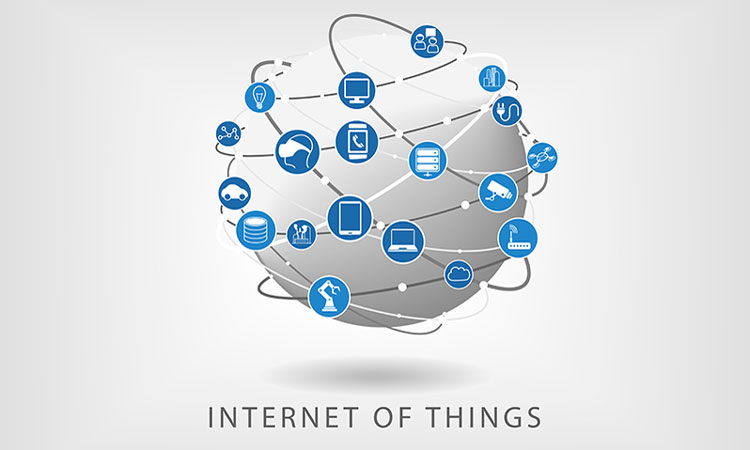
\includegraphics[width=0.7\columnwidth]{images/iot.jpg}
\end{center}
\caption{Overview del paradigma IoT}
\label{fig:iot}
\end{figure}

\section{IoT Enabling Technologies}
\label{sec:iot_enabling_technologies}

L'idea di una rete Internet che consentisse la comunicazione a livello globale tra persone o tra persone e cose o tra cose era già da molto tempo una visione condivsa di quello che sarebbe potuto essere lo sviluppo di Internet. \\
Tale visione è oggi possibile grazie alla diffusione capillare in qualsiasi strumento di piccoli, economici e potenti dispositivi di calcolo. \\
Tuttavia, affinchè una simile rivoluzione tecnologia si paventasse, era necessario superare i tradizionali protocolli di comunicazione tipici della rete Internet e creare conseguentemente delle nuove tecnologie per la comunicazione che fossero ottimizzate per le nuove esigenze.
Va infatti ricordato ancora una volta che la vision dell'IoT sia quella di abilitare una comunicazione tra qualsiasi tipo di dispositivo che abbia al suo interno una unità di calcolo. Questo significa stabilire una comunicazione tra dispositivi eterogenei, dispositivi che assolvono diversi compiti ed adempiono a diverse necessità e che sono molto spesso anche dotati di una diversa e limitata potenza di elaborazione. \\
Di qui la necessità di nuovi protocolli e tecnologie di comunicazione che non solo garantissero la comunicazione sicura di una grossa mole di dati tra un grande numero di dispositivi, ma che fossero anche dei protocolli leggeri dal punto di vista computazionale ed ovviamente economici, così da poter essere integrati in qualsiasi dispositivo, da quelli destinati all'industria a quelli destinati al mercato consumer.
Data la complessità della sfida tecnologica da fronteggiare e considerata l'eterogeneità del problema e delle necessità nei diversi campi applicativi,
sono stati sviluppati e proposti diverse tipologie di tecnologie e protocolli di comunicazione. \\
Tra le più rilevanti nel campo della comunicazione domestica o locale emergono Bluetooth Low Energy \cite{famous:paper_1} and Zigbee \cite{famous:paper_2}. Mentre altri protocolli come WiFi, LowPower Wide Area Networks (LPWA) \cite{famous:paper_3} e le comunicazioni cellulari come 3GPP , 4G o 5G \cite{famous:paper_Grieco_1} hanno uno scope più ampio, abilitando la comunicazione tra dispositivi anche molto distanti tra loro.



\chapter{Sistemi di Crowdsourcing}
\label{chap:due}
Con il termine Crowdsourcing ci si riferisce alla \textit{possibilità di utilizzare i contributi indipendenti di una "folla" per uno scopo, senza che questi siano organizzati a priori in flussi di lavoro} \cite{book:wikipedia_crowdsourcing}.\\
L'evoluzione dell'umanità è stata sempre legata al linguaggio o più in generale alla comunicazione. Attraverso la comunicazione, sia che essa avvenga attraverso i gesti o il linguaggio o Internet, è stato possibile condividere la conoscenza acquisita dagli esseri umani. Ogni uomo ha potuto rendere disponibile la propria conoscenza e la propria esperienza dapprima ai suoi vicini ed ora, attraverso Internet, a tutto il mondo.\\
L'Internet of Things non è altro che l'ennesimo strumento per lo scambio di dati e quindi per la condivisione della conoscenza acquisita. Solo che in questo caso, la conoscenza non viene più acquisita e condivisa tra i soli uomini ma anche tra uomini e macchine e tra macchine e macchine.\\
Di pari passo con la crescita del numero di dispositivi che raccolgono dati, sono anche cresciute le scienze ed i servizi che utilizzano ed analizzano questi dati per trarne da questi delle informazioni. Data la mole dei dati sui quali si opera, questi dati non potrebbero essere analizzati se non che da algoritmi. D'altro canto, questi algoritmi o tecniche di Machine Learning sui dati, fanno un uso massiccio di dati ed inoltre, diventano più accurati all'aumentare del numero di dati che ricevono in pasto. Si crea quindi una doppia relazione tra i sensori e dispositivi IoT connessi alla rete che raccolgono dati di ogni sorta e strumenti di analisi dei dati che, analizzando questi dati, effettuano delle previsioni ed offrono dei servizi i quali, diventano sempre più completi ed accurati quanto più numerosi ed accurati siano i dati a disposizione.
\begin{figure}
	\begin{center}
		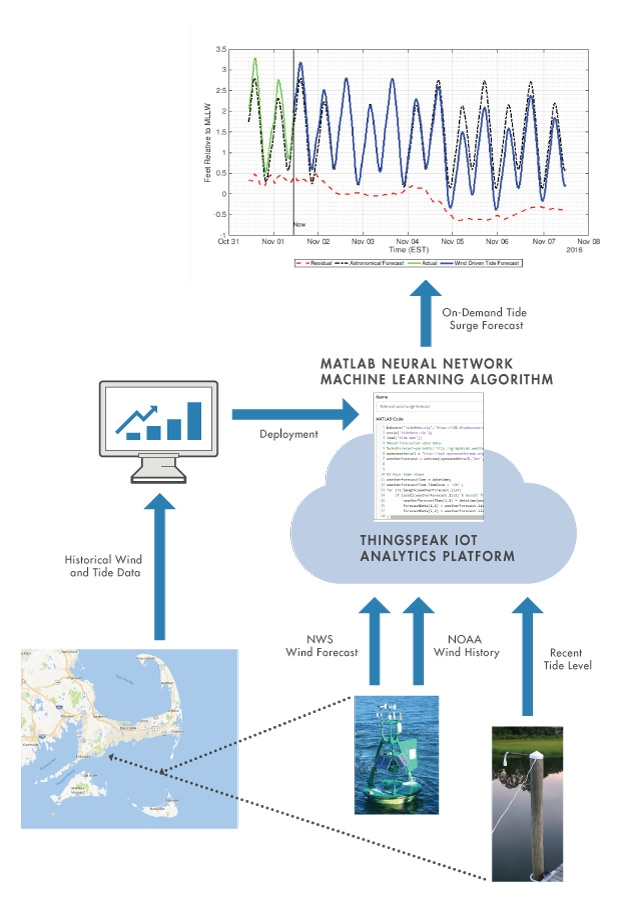
\includegraphics[width=0.5\columnwidth]{images/machine_learning_iot}
	\end{center}
	\caption{Esempio dello sviluppo di un sistema IoT di analisi utilizzando MATLAB, Machine Learning e ThingSpeak \cite{famous:matlab_machine_learning}}
	\label{fig:machine_learning_iot}
\end{figure}
Per soddisfare questa fame di dati e quella che verrà in futuro, per quanto la raccolta dati possa essere automatizzata e distribuita in un numero infinitamente alto di dispositivi, sono necessarie delle risorse ingenti per la distribuzione, manutenzione e creazione di infrastrutture di comunicazione per fare in modo che questi dati siano disponibili ed utilizzabili.
Di qui l'idea del Crowdsourcing di esternalizzare un lavoro o parte di un lavoro ad un gruppo di persone o nel nostro caso, ad un gruppo di cose e persone. L'obiettivo è quello di sfruttare una più grande forza lavoro per il raggiungimento di un certo scopo, ovvero quello della racoclta massiccia di dati. \cite{famous:paper_crowdsourcing_4}
Ricerche dimostrano che ricorrere all'utilizzo del Crowdsourcing, anche al di fuori del mondo IoT, ed in particolare degli approcci di Crowdsourcing legati ai cittadini, possano risultare una fonte affidabile, scalabile e sostenibile per la raccolta di grosse moli di dati. \cite{famous:paper_crowdsourcing_4}
Per chiarire definitivamente il concetto ed i vantaggi del Crowdsourcing, vengono mostrate nella \autoref{sec:crowdsourcing_application} alcune tra le applicazioni più comuni e famose che sfruttano appunto tutta la potenza del Crowdsourcing.

\section{Applicazioni di Crowdsourcing}
\label{sec:crowdsourcing_application}
Attualmente, sono molteplici le applicazioni che sfuttano la potenza messa a disposizione da una \textit{'forza lavoro'} praticamente gratuita ed inesauribile. Queste applicazioni sono talmente comuni ed ottimizzate da non farci nemmeno sospettare di essere noi, con i nostri utilizzi, ad essere la \textit{'forza lavoro'} che produce miliardi di dati e che, molto spesso, quelli stessi dati, dopo opportune analisi, li consuma anche.
Negli esempi contenuti nei paragrafi successivi, sarà subito lampante come queste applicazioni di Crowdsourcing si differenzino principalmente in un aspetto: \textbf{chi genera i dati}. Sono infatti proposte applicazioni nelle quali a generare i dati sono gli umani, condividendo ciò che essi vedono o conoscono. Oppure, ci sono applicazioni nelle quali i dati sono generati dalle macchine, a volte in maniera completamente trasparente all'uomo che spesso ne è addirittura inconsapevole.
\subsection{Google Maps}
Google Maps \textregistered \hspace{2mm} è il celebre servizio offerto da Google che ci consente di orientarci in nuove città, scoprire nuovi posti che potrebbero interessarci, aiutarci a trovare la strada migliore per tornare a casa e guidarci nella navigazione.
Nella fattispecie, il servizio di navigazione offerto da Google Maps \textregistered \hspace{2mm}, si è rivelato ben presto nettamente superiore alle soluzioni di navigazione precedentemente in uso. Questo tutto grazie all'IoT e nella fattispecie ad un sistema di Crowdsourcing tra i più potenti ed avanzati. La feature aggiuntiva di Google Maps \textregistered \hspace{2mm} e di altri servizi simili (Apple Maps \textregistered) sta nel fatto che sono in grado, sulla base della condizione del traffico stimata in real time, di suggerirci la strada migliore per arrivare a casa, in qualsiasi parte del mondo essa sia, nel minor tempo possibile. Per realizzare una simile infrastruttura, sarebbero necessarie centinaia di sensori, sistemi di visione ed antenne per la comunicazione in real time dello stato sul traffico per ogni km di strada, in tutto il mondo. Senza azzardare calcoli, la cifra per la progettazione, sviluppo e manutenzione di un simile impianto sarebbe spropositata persino per Google. Pertanto Google ha deciso di sfruttare il dispositivo IoT più comune, più utilizzato e più diffuso: lo smartphone, lo stesso smartphone che utilizza i servizi offerti da Google Maps \textregistered \hspace{2mm} è utilizzato da Google per ottenere delle stime in real time sul traffico. Di fatto, ogni giorno, miliardi di dispositivi si muovono su tutte le strade del mondo. Questi sono, a tutti gli effetti, dei dispositivi IoT in quanto dotati di sensori, comunicazione attraverso Internet ed una sovrabbondante capacità di calcolo.\\
Non c'è da stupirsi, infatti, se una rete così grande di sensori possa fornire informazioni sufficienti a Google per consigliarci in maniera estremamente accurata di seguire un percorso piuttosto che un altro per tornare a casa evitando così rallentamenti o incidenti.
\begin{figure}
	\begin{center}
		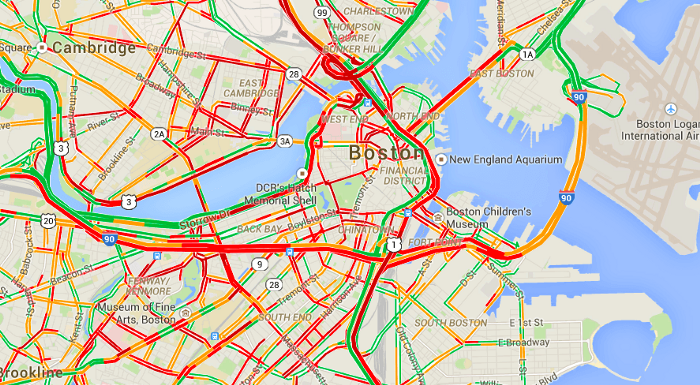
\includegraphics[width=0.7\columnwidth]{images/google_map_traffic}
	\end{center}
	\caption{Indicazione sul livello di traffico stradale nella città di Boston}
	\label{fig:google_map_traffic}
\end{figure}
La capacità di combinare la velocità di un dispositivo con la velocità di altri dispositivi sulle strade, utilizzando migliaia di smartphone in movimento in una area geografica ad un dato periodo di tempo, ha consentito ai servizi offerti da Google di fornire una panoramica affidabile delle condizioni di traffico in real time. Tutto questo ottenuto senza sborsare l'enorme cifra necessaria alla distribuzione di una quantità spropositata di sensori sulla rete stradale di tutto il mondo, ma utilizzando una delle più grandi piattaforme di Crowdsourcing completamente invisibile a coloro che la utilizzano e completamente invisibile a coloro che contribuiscono alla creazione di dati. \cite{patent:google_traffic_info}
\subsection{Linux e Wikipedia}
Un esempio di Crowdsourcing completamente differente da quello mostrato in precedenza, è quello che ha consentito la realizzazione di piattaforme come Wikipedia e del sistema operativo Linux.
In questo caso, infatti, l'utente non solo è consapevole di contribuire alla realizzazione di un progetto distribuito, ma anche deve mettere a disposizione attivamente le proprie competenze per contribuire al progetto.\\
In Wikipedia, ogni utente registrato, è spronato a dare il proprio contributo per l'accrescimento della più grande enciclopedia pubblica e gratuita. La \textit{'forza lavoro'} in questo caso è consapevole del ruolo svolto, della sua importanza e dell'impatto che esso ha sulla comunity di utilizzatori.\\
Allo stesso modo, il sistema operativo Linux, viene sviluppato e manutenuto da una community di sviluppatori, il cui contributo è quello di mettere a disposizione le proprie competenze informatiche per sviluppare e quindi rilasciare il Sistema Operativo in forma Open Source.\\
In entrambi i casi, il sistema Crowdsourcing è stato indispensabile alla creazione del prodotto finito.
Se pensiamo a Wikipedia, in essa sono contenute più di 320 milioni di pagine, tradotte in 280 lingue, uno sforzo immane se questo lavoro fosse toccato ad una sola persona o ad una sola azienda. Invece, sfruttando il Crowdsourcing, si raccoglie tutta la conoscenza acquisita da qualsiasi uomo in qualsiasi parte del mondo, in qualsiasi istante di tempo. \cite{book:wikistats}\\
I numeri di Linux, sono altrettanto impressionanti, si stima infatti che al 2018, Linux fosse composto da oltre 25 milioni di righe di codice, scritte da più di 19 mila diversi contributori. (fonte: \url{https://linux.slashdot.org/})
Ancora una volta, questi numeri sono possibili grazie ad una community che collabora per il raggiungimento di un certo fine che, in questo caso, piuttosto che finalizzato alla raccolta dei dati, è finalizzato alla condivione della conoscenza e delle competenze.

\section{Crowdsourcing ed Internet of Things}
Ora che sono chiare le potenzialità offerte dal Crowdsourcing, è necessario affrontare un altro tema che consentirà di avere una più chiara visione sul legame Crowdsourcing ed IoT dal quale sarà possibile trarre utili informazioni necessarie alla progettazione fatta nel \autoref{chap:tre}.\\
Sebbene evidenti i vantaggi delle piattaforme di Crowdsourcing negli esempi mostrati nella \autoref{sec:crowdsourcing_application}, vanno tuttavia effettuate alcune considerazioni ed accorgimenti da intraprendere quando si utilizzano simili strumenti.\\
Il mondo dell'Internet of Things, si adatta perfettamente a quella che è l'idea alla base del Crowdsourcing : \textit{Esternalizzazione di una parte del lavoro ad un gruppo di persone, le quali, con contributi indipendenti e non organizzati lavorano per uno scopo comune}. Se ci si sforza ad estendere questa definizione non solo alle persone ma anche alle cose, è possibile vedere come questa nuova definizione del Crowdsourcing applicata agli oggetti, bene si adatti con il paradigma dell'Internet of Things.
Se grazie agli strumenti, sensori, protocolli e sistemi integrati offerti dal paradigma IoT è possibile garantire che qualsiasi oggetto possa raccogliere dati e condividerli attraverso Internet, il Crowdsourcing ci suggerisce che tutti questi dati, raccolti come contributi indipendenti da un grande numero di dispositivi, possano essere raggruppati ed utilizzati insieme per il raggiungimento di un più grande scopo. \cite{famous:paper_crowdsourcing_4} \cite{famous:paper_crowdsourcing_2}\\
Nella \autoref{sec:crowdsourcing_application} è stata volutamente omessa una informazione. Sebbene sia vero che senza il Crowdsourcing sarebbe stato impossibile per Linux raggiungere le 25 milioni di righe di codice e per Wikipedia sarebbe stato impossibile raggiungere le 320 milioni di pagine, è anche vero che il contributo dei 19 mila sviluppatori di Linux e dei 4 milioni di utenti registrati in Wikipedia vada gestito e regolamentato. Si rende cioè necessario trovare una sorta di Protocollo o di Interfaccia comune che tutti i contributori, sebbene indipendenti, debbano seguire ed adottare per contribuire al progetto.\\
In Linux questa interfaccia risiede nel software Git per il source control. In questo modo ogni sviluppatore che contribuisce al progetto Linux può clonare \footnote{Termine utilizzato per indicare l'ottenimento di una copia di un progetto globale in una propria cartella locale} o fare un branch \footnote{Termine che indica l'esecuzione di una diramazione di un certo progetto, in un certo stato} del progetto esistente, aggiungere le proprie modifiche ed effettuare nuovamente un commit \footnote{Termine che indica la conferma dell'esecuzione di una modifica ad un dato progetto} sul server così che tutti possano prendere visione delle modifiche apportate. Soltanto dopo aver verificato che le modifiche di un certo utente siano conformi al task richiesto, non introducano problemi o bug e non comportino un rischio per la sicurezza, ne viene effettuato il merge \footnote{Termine che indica l'unione di due versioni dello stesso codice} all'interno della directory principale.\\
Analogamente, in Wikipedia, è necessario verificare la veridicità e la correttezza dei contributi di ciascun utente. A tal proposito, Wikipedia si affida ad un'altra forma di Crowdsourcing, questa volta realizzata non solo da utenti registrati ma anche da coloro che usufruiscono del servizio che possono segnalare argomenti che ritengono sbagliati o non completi.\\
Questa necessità di realizzare una Interfaccia o un Protocollo comune a tutti i contributori di una piattaforma di Crowdsourcing si rende necessaria non solo nelle applicazioni dove i contributori sono umani, ma anche in quelle dove i contributori sono macchine.\\
Come evidenziato nel \autoref{chap:introduzione}, la forza dell'Internet of Things è quella di abilitare una comunicazione ed uno scambio dati tra dispositivi eterogenei. Con eterogenei si intende una differente potenza di calcolo, dotazione sensoristica, funzionamento, costo e casa produttrice. Il risultato di questa eterogeneità è che non esiste un modo comune di identificare un particolare dispositivo all'interno di una piattaforma di Crowdsourcing, ovvero il tipo del dispositivo, il costruttore e quali dati sono prodotti non sono informazioni regolate da uno Standard comune. \cite{famous:paper_crowdsourcing_4} Una difficoltà aggiuntiva se si realizza una piattaforma di Crowdsourcing con dispositivi IoT, sta nel fatto che sia necessario gestire e legittimare l'accesso e la produzione dei dati. Analogamente a quanto fatto da Wikipedia e Linux, è cioè necessario gestire i contributi dei singoli ed ulteriormente verificare che essi siano corretti e conformi.
I problemi legati allo sviluppo di una piattaforma di Crowdsourcing legata a dispositivi IoT sono quindi:
\begin{enumerate}
	\item \textbf{Interoperabilità Semantica :} L'IoT è una tecnologia \textit{'industry driven'} nella quale ogni costruttore realizza la sua piattaforma IoT. In più, la maggior parte delle soluzioni IoT sono case-centric con la conseguente creazione di \textit{'IoT Silos'} i quali, per comunicare tra loro e scambiarsi dati, hanno bisogno di una interoperabilità \textit{'Inter-Silos'}. Si rende necessario che ogni Protocollo o Standard debba considerare la varietà dei dispositivi, il loro contesto di utilizzo ed i dati emessi. La sfida nel dominio IoT è dovuta alla presenza di una varietà di ontologie che trattano vari aspetti dei sensori e delle grandezze da misurare (diversa portata, granularità e generalità). Questo complica lo sviluppo di una ontologia formale o di un Protocollo di comunicazione comune a tutti i dispositivi.
	\item \textbf{Condivisione dei Dati e Controllo degli Accessi :} Un'altra grande sfida per la ricerca nel campo dell'IoT è quella di garantire la privacy degli utenti e la protezione dei dati personali, specialmente in sistemi nei quali si effettua raccolta, gestione e condivisione dei dati. L'identificazione e la gestione di miliardi di dispositivi connessi tra loro ed il mantenimento di una comunicazione affidabile e sicura, rappresentano un punto critico da regolamentare.
	Questo richiede sia lo sviluppo di una policy che regolamenti la comunicazione ma anche richiede uno sviluppo tecnologico per la condivisione sicura ed affidabile con protocolli leggeri ed interoperabili.
	\item \textbf{Elaborazione di Politiche Democratiche :} Alcuni domini specifici nei quali l'IoT si sta diffondendo come l'healthcare e le smart cities, sono campi di applicazione nei quali gli individui operano non soltanto come data providers, ma essi partecipano attivamente nella risoluzione di problemi, condivisione di soluzioni e formulazione di leggi e regolamenti. Si rende quindi necessario adattare il comportamento e i Protocolli o Standard di comunicazione alle particolari politiche democratiche ed ulteriormente al particolare campo di applicazione.
\end{enumerate}







\chapter{Progetto del Sistema}
\label{chap:tre}
Nei capitoli precedenti è stata offerta una panoramica sugli strumenti che il paradigma IoT mette a disposizione e su come alcune compagnie utilizzino piattaforme di Crowdsourcing per fornire risorse e servizi altrimenti impensabili.\\
In questo capitolo, saranno trattate la progettazione e le scelte architetturali che hanno portato alla prototipazione di un Software che sfrutti il paradigma IoT e tecniche di Crowdsourcing per offrire un servizio legato al mondo dell'Automotive. In questo capitolo, tuttavia, piuttosto che alla realizzazione di un prodotto finito, ci si focalizzerà sulle motivazioni che hanno portato ad alcune scelte progettuali piuttosto che ad altre. Tale fase di progettazione, essendo di carattere completamente generale, potrà essere utilizzata anche per lo sviluppo di altri sistemi in altri campi applicativi che facciano uso di tecniche di Crowdsourcing applicate a dispositivi IoT.\\

\section{Idea Generale}
\label{sec:general_idea}
Recentemente, notevole importanza viene posta ai cosiddetti Intelligent Transportation System (ITS) sia da parte delle amministrazioni pubbliche ed europee (2019/40/EU \cite{famous:paper_europe}) che nel mondo della ricerca. \cite{famous:paper_bonvoyage}
In \cite{famous:paper_europe}, infatti, viene definito un framework per le specifiche di sviluppo che rendano interoperabili le piattaforme ITS anche attraverso differenti organizzazioni. La necessità è quella di fornire informazioni sul traffico in real-time per il territorio Europeo.\\
Avendo a mente questa necessità, in questo lavoro di tesi si intende progettare e sviluppare un Software che, raccogliendo dati sulla navigazione da dispositivi eterogenei e, raggruppando questi dati in una piattaforma di Crowdsourcing, possa sottoporli ad analisi e ricavare così delle informazioni sul livello del traffico in una data area geografica.
I dati raccolti possono essere di diversa natura, proprio perchè diversa è la natura dei dispositivi che possono raccogliere ed inviare questi dati. Alcune informazioni possono riguardare:
\begin{itemize}
	\item Dati legati alle condizioni del traffico
	\item Dati provenienti da vari sensori disposti sulla rete stradale (es. stazioni meteo)
	\item Dati provenienti da dispositivi che transitano temporaneamente sulle strade (Smartphone, Tablet, Sistemi di Infotainment nelle automobili)
	\item Dati provenienti da videocamere a circuito chiuso (CCTV)
\end{itemize} 
Dunque, proprio data l'eterogeneità di dispositivi che parteciperanno alla fase di raccolta dati, sarà necessario anche anlizzare alcune tecniche e Protocolli che consentano ad una così eterogenea estrazione di dispositivi di poter raccogliere dati ed inviarli in un formato comune e quindi comprensibile.
Infine, una volta creato e popolato in real time il dataset, questi dati saranno resi disponibili per delle query geo-referenziate, in modo tale che, una utenza privata o una organizzazione per il controllo del traffico, possa accedere ad i dati più recenti sul traffico di una certa area geografica.\\
Nella fattispecie, la fase di progettazione riguarderà:
\begin{itemize}
	\item Raccolta dei Dati
	\item Formattazione dei Dati in una Interfaccia condivisa tra dispositivi eterogenei
	\item Geo-Referenziare i Dati
	\item Invio dei dati Geo-Referenziati ad un Middleware IoT
	\item Storing dei dati Geo-Referenziati in Database opportunamente progettati
	\item Gestione delle query Geo-Referenziate al Database
\end{itemize} 
\begin{figure}
	\begin{center}
		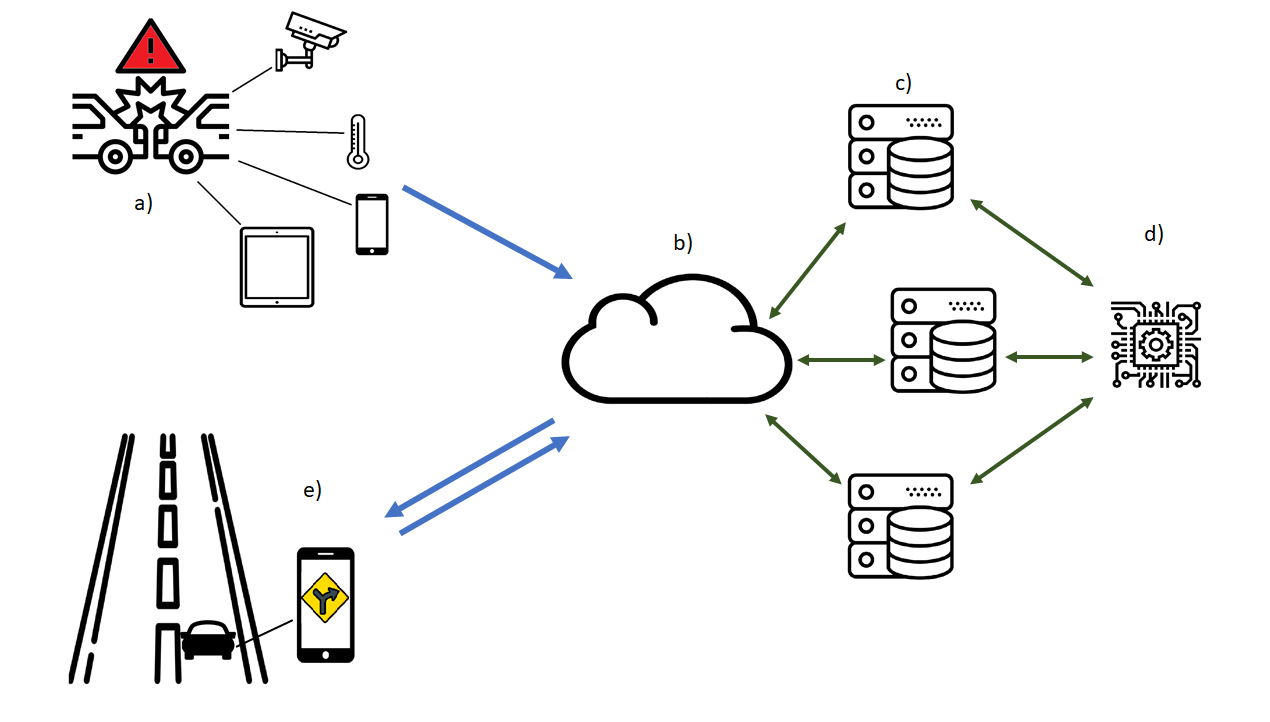
\includegraphics[width=0.8\columnwidth]{images/schema_fin}
	\end{center}
	\caption{Schema del prototipo. a) Raccolta dei dati attraverso un sistema eterogeneo di dispositivi. b) Condivisione dei dati in un Middleware IoT. c) Storing dei dati all'interno di Databases d) Analisi sui dati. d) Query Geo-Referenziata sulle condizioni di traffico. }
	\label{fig:application_schema}
\end{figure}

\section{La Raccolta dei Dati}
Il primo passo per l'implementazione di un sistema come quello proposto nella \autoref{sec:general_idea} è quello dello studio ed analisi dei dati necessari e la conseguente raccolta degli stessi. \\
Lo sviluppo delle tecnologie legate al mondo dell'IoT ha prodotto tutto un movimento tecnologico per la creazione di nuovi dispositivi e per il miglioramento di quelli esistenti. Questo ha consentito lo sviluppo di competenze tecnologiche nella realizzazione di unità di calcolo, circuiti integrati, sensori e strumenti di comunicazione sempre più avanzati ed economici. Questo movimento ha consentito inoltre di incrementare la diffusione di componenti elettroniche la cui potenza e costo li rendono disponibili all'utilizzo in qualsiasi applicazione. \\
In riferimento allo sviluppo di un sistema come quello ideato nella sezione \autoref{sec:general_idea}, si richiede che un numero molto elevato di sensori venga disposto sulla rete stradale in maniera capillare, così da poter avere dati affidabili ed in real-time sulla condizione del traffico in tutto il territorio. Alcuni di questi sensori sono già presenti ma sono in numero talmente basso che, con i dati da essi estratti, si potrebbero solamente ottenere informazioni parziali sul traffico su una porzione molto limitata del territorio.
\begin{figure}
	\begin{center}
		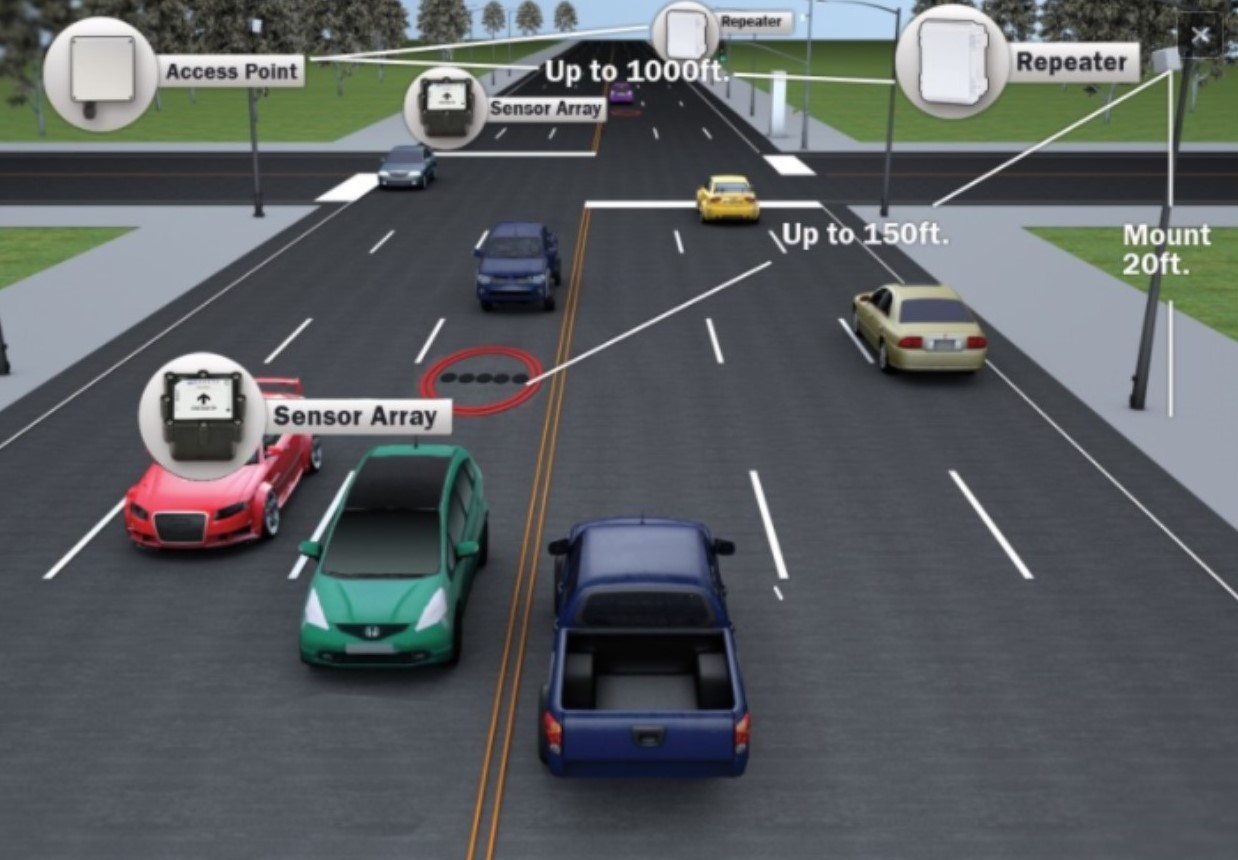
\includegraphics[width=0.7\columnwidth]{images/traffic_sensor}
	\end{center}
	\caption{Principio di funzionamento dei sensori attualmente in uso per la misura del livello di traffico}
	\label{fig:traffic_sensors}
\end{figure}
Le difficoltà principali nello sviluppo di una piattaforma per il controllo del traffico sono ovviamente quelle legate ai costi per la distribuzione di una rete di sensori che copra tutta la rete stradale.
Pertanto, è necessario trovare altre soluzioni che possano risultare più sostenibili ed anche scalabili.
Come evidenziato nel \autoref{chap:due}, uno dei principali vantaggi di una piattaforma di Crowdsourcing è proprio quello di garantire che, attraverso il contributo non organizzato dei singoli, si possa raggiungere un obiettivo comune riducendo di fatto i costi.\\
Attualmente, infatti, la rete stradale è già ampiamente invasa da un numero estremamente elevato di sensori i quali sono diffusi in maniera capillare e senza costi aggiuntivi: gli Smartphone (o Tablet). \\
Gli Smartphone sono il più evidente esempio della diffusione di componenti elettroniche  i quali, nelle loro evoluzioni hanno integrato al loro interno un numero sempre maggiore di sensori, diventando sempre più accurati e miniaturizzati.
\begin{figure}
	\begin{center}
		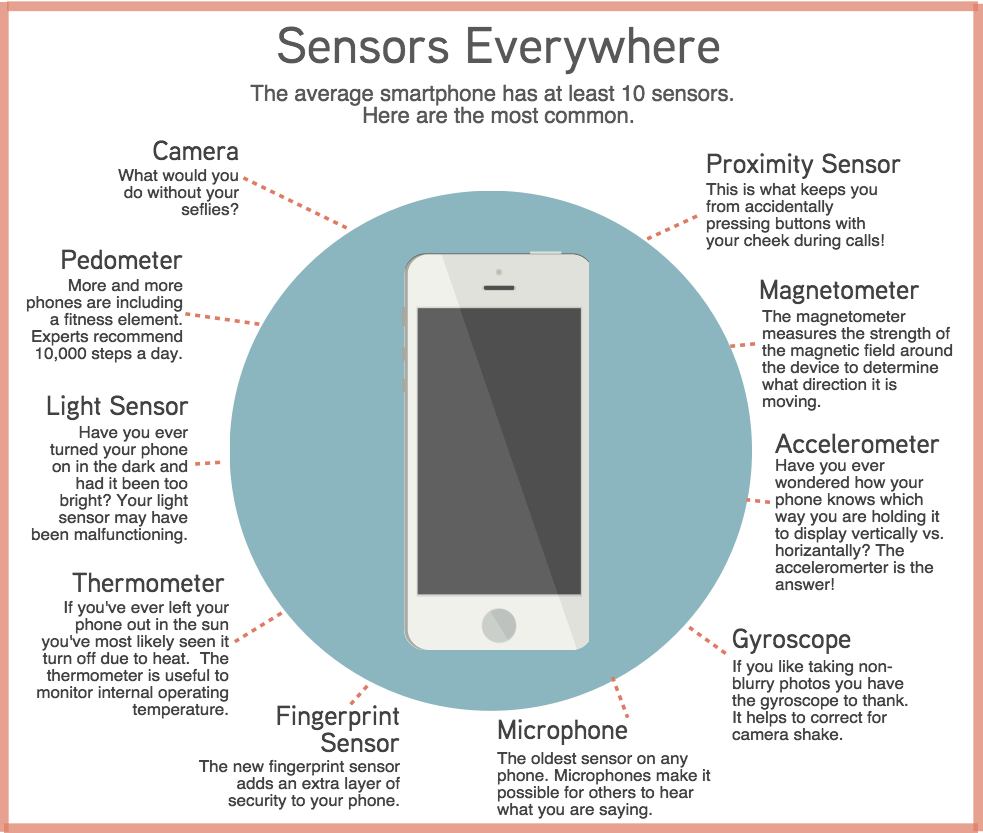
\includegraphics[width=0.8\columnwidth]{images/smartphone_sensors}
	\end{center}
	\caption{Crescita della disponibilità di sensori nell'equipaggiamento di uno smartphone fonte: CornerAlliance}
	\label{fig:smartphone_sensors}
\end{figure}
Sebbene il mercato degli smartphone sia molto eterogeneo dal punto di vista della dotazione hardware e del sistema operativo, generalmente si avranno sempre a disposizione alcune tipologie di sensori che possiamo classificare in funzione della grandezza fisica che essi misurano:
\begin{itemize}
	\item Termometro
	\item Accelerometro
	\item Giroscopio
	\item Microfono
	\item Camera
	\item GPS
\end{itemize}
Con l'aggiunta, in dispositivi più avanzati di:
\begin{itemize}
	\item[$\blacksquare$] Pedometro
	\item[$\blacksquare$] Prossimità
	\item[$\blacksquare$] Impronte Digitali
	\item[$\blacksquare$] Magnetometro
\end{itemize}
Effettivamente, la sensoristica di cui è dotato un singolo smartphone non sarebbe in nessun modo in grado di stimare autonomamente il livello del traffico o l'eventuale presenza di incidenti. Tuttavia, una piattaforma che raccolga i dati di un gran numero di dispositivi e che utilizzi degli algoritmi di analisi dei dati, sarebbe in grado di effettuare delle stime sul livello del traffico in un' area geografica. Questo è quello che viene proposto in \cite{famous:paper_smartphone_traffic_detection} dove viene analizzata una piattaforma per la raccolta dei dati relativi al traffico proveniente da un gran numero di smartphone e ne viene anche analizzato il rischio per la sicurezza di un utente che contribuisca ad una simile piattaforma dovendo condividere, tra gli altri, anche i dati relativi alla propria posizione.\\
Nel caso del prototipo ideato nella \autoref{sec:general_idea}, non si vuole soltanto realizzare una piattaforma che raccolga dati provenienti da smartphone, ma si vuole fare in modo che questa piattaforma sia adatta anche a raccogliere dati provenienti da infrastrutture stradali ed autostradali per il monitoraggio del traffico e per la comunicazione del livello di traffico. Si vuole cioè raccogliere in un'unica piattaforma i dati provenienti dai sensori stradali per il traffico come quello mostrato in \autoref{fig:traffic_sensors}, quelli provenienti da stazioni meteo, smartphone, tablet, computer di bordo di automobili, stazioni di monitoraggio del traffico e così via. Sebbene nella fase di prototipazione ci si focalizzerà principalmente sulla raccolta dati da smartphone e della conseguente trasmissione degli stessi secondo un predefinito formato, tutte le scelte progettuali sono pensate per essere compatibili anche per la raccolta dati dai diversi dispositivi precedentemente elencati.



\subsection{Accesso ai Sensori di uno Smartphone}
L'aumento del numero dei sensori, l'aumento della loro accuratezza ed affidabilità, ha portato alla nascita di servizi che utilizzassero tutte o alcune delle letture fornite dai sensori per offrire dei servizi all'utenza.\\
Alcuni di questi servizi consentono ad esempio di monitorare la qualità del proprio sonno, il numero di Kcal bruciate ogni giorno, regolare in modo automatico la luminosità e la gamma di colori del proprio schermo per salvaguardare gli occhi dell'utilizzatore ed una serie di altri infiniti servizi, tutti possibili sulla base dei dati provenienti da uno o più sensori.\\
\begin{figure}
	\begin{center}
		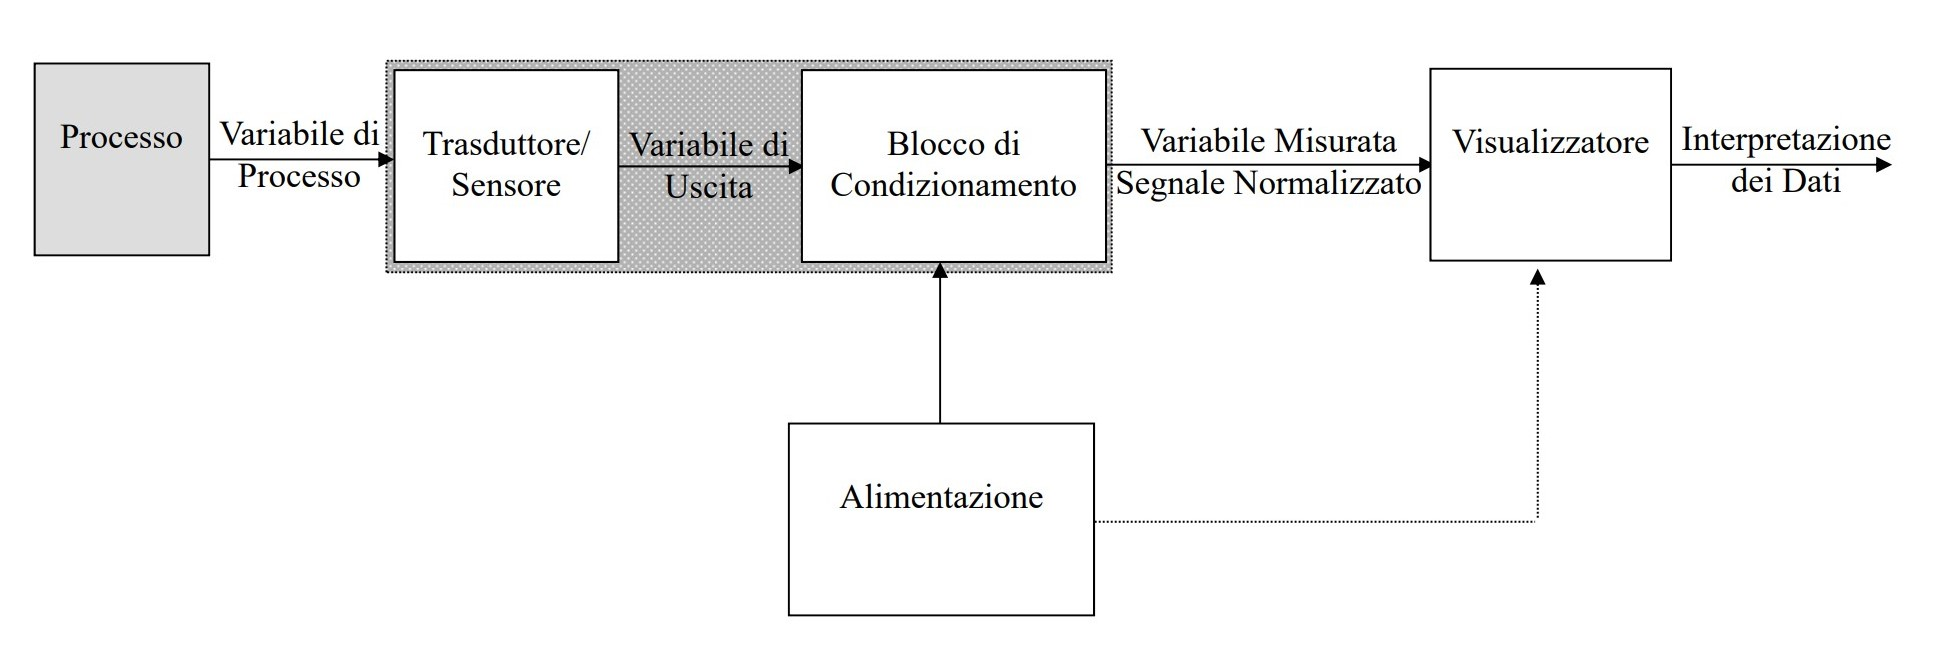
\includegraphics[width=0.9\columnwidth]{images/attivissimo}
	\end{center}
	\caption{Schema generale di un sistema di misura}
	\label{fig:attivissimo}
\end{figure}
\begin{figure}
	\begin{center}
		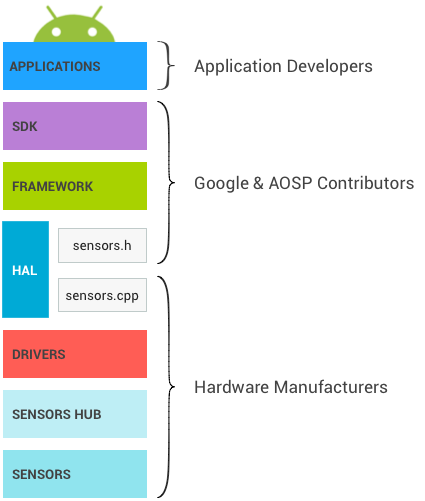
\includegraphics[width=0.55\columnwidth]{images/android_sensors}
	\end{center}
	\caption{Estratto dello stack utilizzato nel sistema operativo Android per rendere disponibili le letture dei sensori ad applicazioni e servizi}
	\label{fig:android_sensors}
\end{figure}
Questi servizi o applicazioni non sono altro che l'ultimo step di una struttura verticale nella quale, ai primi livelli si trovano effettivamente le componenti hardware del sensore che producono una uscita elettrica. Si rende necessario poi filtrare, amplificare e condizionare questo segnale elettrico al fine di renderlo comprensibile e trasmissibile come in \autoref{fig:attivissimo}. La variabile fisica o variabile di processo che si intende misurare viene quindi trasdotta o convertita in un'altra forma (generalmente elettrica) che è più semplice da trasmettere ed elaborare. Questa variabile di uscita prodotta dal blocco sensore e trasduttore non è tuttavia ancora adatta ad essere utilizzata. Questa subirà quindi un nuovo processo di condizionamento nel quale verrà filtrata, amplificata e linearizzata. Di qui il sistema operativo si occupa di interpretare ed eventualmente tradurre in un diverso formato le letture dei sensori in modo da renderle disponibili attraverso una interfaccia alle applicazioni e servizi dei livelli superiori che ne fanno richiesta. Tali applicazioni o service provider saranno quindi solo i consumatori finali di questi dati dai quali estrarranno le informazioni da mostrare all'utente finale che usufruisce del servizio.
Come evidente, nello stack utilizzato dal sistema operativo per smartphone Android \autoref{fig:android_sensors} viene offerto agli sviluppatori che realizzano servizi ed applicazioni una interfaccia diretta e standardizzata per l'utilizzo delle letture provenienti dai sensori. A prescindere dal sistema operativo utilizzato e dal tipo di sensori di cui è dotato lo smartphone, sarà offerto agli sviluppatori una interfaccia chiamata SDK ovvero Software Development Kit che indica un insieme di strumenti per lo sviluppo e la documentazione di software. In questo modo, coloro che si occupano di fornire servizi basati sulle letture di sensori, non dovranno preoccuparsi di elaborare, tradurre e condizionare l'uscita del sensore, ma solo di utilizzarla. \cite{developer:android} \cite{developer:apple}

\subsection{Parametri di Qualità dei Sensori}
\label{subsec:quality_param}
Ai sensori è generalmente richiesto di funzionare in ambienti ostili all'uomo e spesso ostili anche all'elettronica. Inoltre, un sensore sarà ritenuto tanto migliore quanto più esso riuscirà ad essere sensibile ad una sola grandezza ed insensibile a tutte le altre grandezze o rumore che possono disturbarne la misura. \cite{book:slide_Attivissimo} \cite{book:sensori_trasduttori} \\
Si può quindi sintetizzare che la \textbf{qualità di un sensore} sia determinata dalla sua sensibilità alla grandezza che si vuole misurare e dalla sua insensibilità a tutte le altre grandezze fisiche ambientali.
Essendo interessati alla valutazione delle prestazioni di un sensore in modo da poterne valutare la sua affidabilità e la qualità delle sue letture, va considerato che l'accurateza del dispositivo può variare con altre grandezze di influenza (temperatura, umidità, ecc.) e che spesso, si perviene alla misura di una grandezza fisica di interesse in maniera indiretta, introducendo così una propagazione del'errore.
\begin{figure}
	\begin{center}
		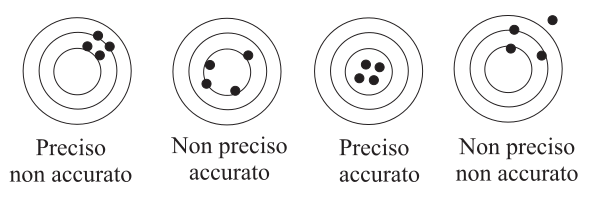
\includegraphics[width=0.9\columnwidth]{images/accuracy_precision}
	\end{center}
	\caption{Differenza tra la definizione di Precisione e quella di Accuratezza di una misura}
	\label{fig:accuracy_precision}
\end{figure}
Una prima valutazione sulla qualità di un sensore può essere effettuata attraverso due indici: \textbf{responsivity} e \textbf{detectivity}.\\
La \textbf{responsivity} o \textbf{sensitivity} rappresenta l'efficienza di trasduzione del sensore ed è normalmente espressa come il rapporto di due unità di misura, in genere differenti.
\begin{center}
	\begin{equation}
		r = \frac{\partial S\textsubscript{o}}{\partial S\textsubscript{i}} \quad \big[S\textsubscript{o} \textbackslash S\textsubscript{i}\big]
	\end{equation}
\end{center}
La \textbf{detectivity} rappresenta la capacità di un sensore di rendere disponibile un segnale dipendente dalla grandezza di ingresso e di tenerlo distinto dal rumore da esso stesso prodotto. Il suo valore dipende dal \textit{noise floor} ed è legato alla soglia o minimo segnale rilevabile. Si misura come il reciproco dell'unità di misura dell'ingresso.
\begin{center}
	\begin{equation}
	d = \frac{S\textsubscript{o}\textbackslash N\textsubscript{o}}{S\textsubscript{i}} = \frac{r}{N\textsubscript{o}} \quad \big[S\textsubscript{i} ^{-1}\big]
	\end{equation}
\end{center}
Queste informazioni, saranno utili al fine dello sviluppo del prototipo in quanto, dal momento che la piattaforma ideata nel \autoref{sec:general_idea} si occuperà di raccogliere i dati provenienti da un numero molto elevato di dispositivi eterogenei, questo significa anche che le letture dei sensori provenienti dai diversi sensori saranno qualitativamente eterogenee.\\
Pertanto, un primo requisito, sarà quello di valutare i parametri di qualità relativi alle letture dei sensori di ciascun dispositivo ed eseguire in questo modo un primo filtraggio dei dati in modo da escludere dall'analisi quelle letture affette da un grado di incertezza troppo elevato o non compatibile con l'analisi effettuata. Nel caso degli smartphone e tablet, queste informazioni sono messe a disposizione all'interno del SDK.

\subsection{Filtraggio delle Letture dei Sensori}
\label{subsec:filtering_sensor}
Nella \autoref{fig:attivissimo} è possibile notare come nel sistema di misura sia presente una componente che si occupi di filtrare, amplificare e linearizzare l'uscita fisica del sensore: il Blocco di Condizionamento. Questo blocco è generalmente di tipo software ed è realizzato ad-hoc per il particolare sensore e per il particolare utilizzo. Il suo scopo è quello di portare il segnale in uscita dal sensore in un formato compatibile con il dispositivo di elaborazione che lo segue riducendo al massimo gli effetti negativi di carico. \cite{book:slide_Attivissimo} Allo stesso modo, anche per quanto riguarda i sensori di cui sono dotati gli Smartphone, è necessario che le relative uscite vengano condizionate in maniera opportuna in funzione della particolare applicazione.\\
Prima però è necessario effettuare un approfondimento sui sensori che possono equipaggiare uno smartphone (e che sono necessari alla predizione delle condizioni stradali). All'interno degli smartphone, infatti, è possibile incontrare due diverse tipologie di sensori:
\begin{itemize}
	\item Sensori Hardware
	\item Sensori Software
\end{itemize}
Questa distinzione, sebbene non evidente all'utente finale, produrrà diverse tipologie di dati che dovranno quindi essere trattati diversamente.\\
I \textbf{Sensori Hardware} sono componenti fisiche che sono effettivamente montate all'interno di uno smartphone. Pertanto, le letture di questi sensori provengono dalla misura di una certa grandezza fisica attraverso un sistema di misura come quello mostrato in \autoref{fig:attivissimo}. Un esempio ne sono l'accelerometro, il magnetometro ed il sensore per l'intensità luminosa.\\
I \textbf{Sensori Software} non sono sensori fisici composti cioè da componenti elettroniche che trasducano una certa grandezza fisica. Questi sensori, emulano il comportamento di un sensore hardware ma le loro uscite sono spesso derivate da uno o più sensori hardware, opportunamente rielaborate via software. Un esempio ne sono sensore di orientamento, vettore di rotazione, pedometro.\\
Sebbene questa distinzione sia completamente invisibile a coloro che utilizzano questi dati e sia anche invisibile a coloro che sviluppano applicazioni e servizi sfruttando l' SDK messo a disposizione dal sistema operativo, è necessario tenerla a mente perchè i dati in uscita dalle diverse tipologie di sensori dovranno essere trattati diversamente. 
I dati in uscita dai sensori software sarnno infatti direttamente utilizzabili in quanto hanno già subito un processo di condizionamento proprio perchè, per definizione, sono derivati da altri sensori hardware.
Si rende invece necessario sviluppare un sistema di filtraggio ed eventualmente linearizzazione per le letture dei sensori hardware.\\
Il problema dei sensori hardware è che la frequenza con la quale le  uscite variano il loro valore è così elevata che, se mappassimo tutte queste piccole variazioni (Rumore), i valori oscillerebbero notevolmente. Più in generale, le letture provenienti dai sensori sono ricevute con una diversa frequenza ma, i picchi da essa raggiunti, sono troppo elevati.
\begin{figure}
	\begin{center}
		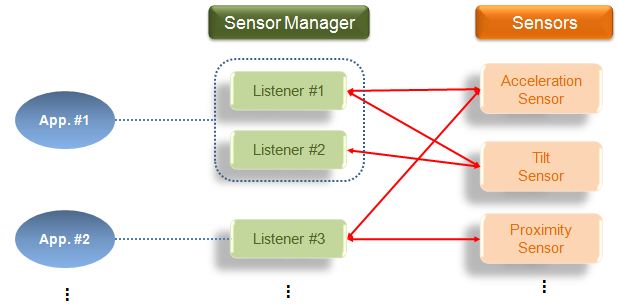
\includegraphics[width=0.9\columnwidth]{images/sensor_listener}
	\end{center}
	\caption{Principio con il quale nel sistema operativo Android è possibile recuperare le letture di un sensore ed utilizzarle in una applicazione. \cite{developer:android}}
	\label{fig:sensor_listener}
\end{figure}
Il processo che viene seguito nel sistema operativo Android per rendere disponibile la lettura di un sensore ad una applicazione o servizio che ne faccia richiesta è quello di instanziare un SensorListener il cui ruolo è appunto quello di restare in ascolto sull'uscita di un dato sensore e di notificare la applicazione nonappena venga rilevata una variazione del valore misurato dal sensore. La frequenza con la quale questo processo avviene dipende dalla velocità del sistema operativo e dalla capacità computazionale del dispositivo. Questo significa che dispositivi con una maggiore capacità di calcolo interrogheranno un numero maggiore di volte il sensore e riceveranno un numero maggiore di risposte affette, inevitabilmente, da rumore. Questo significa che è necessario utilizzare i soli valori necessari ed utili e filtrare il rumore.\\
La soluzione è l'applicazione di un filtro passa-basso sulle letture provenienti dai sensori in modo che esso consenta il passaggio alle sole basse frequenze del segnale e ne attenui il valore alle frequenze superiori a quella di taglio.\\
Si prenda ad esempio l'accelerometro di uno smartphone le cui letture indicano l'accelerazione del dispositivo rilevanta in un predefinito sistema di riferimento.
\begin{figure}
	\begin{center}
		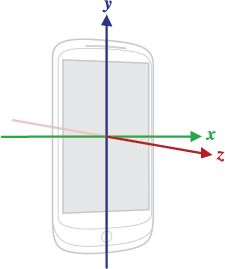
\includegraphics[width=0.3\columnwidth]{images/accelerometer}
	\end{center}
	\caption{Sensore di accelerazione a bordo di uno smartphone}
	\label{fig:accelerometer}
\end{figure}
A causa di un disturbo esterno come fattori ambientali o jerks o vibrazioni, viene aggiunto alla lettura del sensore una gran quantità di rumore. Queste componenti ad alta frequenza del segnale, provocano un'ampia oscillazione dei valori letti dal sensore. Questi disturbi, potrebbero essere tollerabili nella maggior parte delle applicazioni ma se si vogliono ottenere delle migliori letture è necessario progettare e sviluppare un filtro passa-basso che filtri a livello software le uscite di sensori hardware. In questo modo, è possibile filtrare le componenti di rumore ad alta frequenza utilizzando un opportuno valore di soglia.\\
\begin{lstlisting}[language=Java, label= code:low_pass_filter, caption=Pseudo-codice relativo all'implementazione di un filtro passa-basso]
for i from 1 to n
	y[i] :=y [i-1] + a*(x[i] - y[i-1])
end
\end{lstlisting}
Il \autoref{code:low_pass_filter} corrisponde ad una implementazione di un filtro passa-basso che prenda l'uscita \textit{y} di un sensore e la filtri con un filtro passa-basso avente \textit{a} come coefficiente di soglia.
La scelta del parametro \textit{a} dipende da quanto si intende dimensionare la frequenza di taglio del filtro. Quanto più essa sarà alta, tanto più rumore entrerà nel filtro viceversa, quanto più sarà bassa tanto più lento sarà il segnale. In \cite{developer:android} viene proposta una soluzione intermedia con la scelta del parametro \textit{a = 0.25}.

\section{Il Protocollo DATEX}
La raccolta dei dati è solo una piccola porzione del problema. Per ottenere il massimo da questi dati è necessario condividerli in modo da sfruttare le potenzialità delle piattaforme di Crowdsourcing nelle quali, le analisi effettuate su un gran numero di dati potrebbero fornire delle deduzioni e previsioni molto più accurate e significative.
Si rende quindi necessaria una comunicazione tra i dispositivi che si occupano della raccolta dati.\\
Diventa quindi necessario abilitare la comunicazione tra tutti i diversi dispositivi che si occupano della raccolta dati considerando la loro eterogeneità in termini di:
\begin{itemize}
	\item Capacità computazionale
	\item Sensoristica a disposizione
	\item Grandezze fisiche misurate
	\item Qualità delle letture dei sensori
	\item Costruttore del dispositivo
\end{itemize}
DATEX (da Data Exchange) è il protocollo che abilita la comunicazione tra dispositivi eterogenei per la condivisione di dati legati al traffico stradale ed autostradale. Questo protocollo fa in modo che differenti dispositivi possano comunicare tra loro e con un Middleware, definendo cioè uno Standard per la comunicazione condiviso tra tutti i partecipanti alla comunicazione.\\
Nella fattispecie, DATEX è il linguaggio utilizzato nella Comunità Europea per lo scambio di informazioni legate al traffico in modo da consegnare informazioni comprensibili all'utenza finale. DATEX è infatti stato progettato e sviluppato come un sistema per lo scambio di dati dalla Comunità Europea per la standardizzazione dell'interfaccia di comunicazione tra i gestori di strade ed autostrade, i produttori dei dati in strade ed autostrade e gli utilizzatori dei servizi sul traffico. \cite{famous:paper_datexii}\\
Una prima versione del Protocollo DATEX I è stata iniziata già nel 1990 mossa dalla necessità di un meccanismo per lo scambio di dati tra centri per il monitoraggio del traffico e gli operatori stradali. Ben presto, tuttavia, dato lo sviluppo tecnologico del XXI secolo, è sorta la necessità di integrare in questo standard anche i fornitori di servizi. Per questo motivo, viene sviluppato lo standard DATEX II con lo scopo di distribuire le informazioni sul traffico indipendentemente dalla lingua e dall'aspetto. In questo modo, viene eliminata la probabilità che nascano delle incomprensioni o errori di traduzione.\\
\begin{figure}
	\begin{center}
		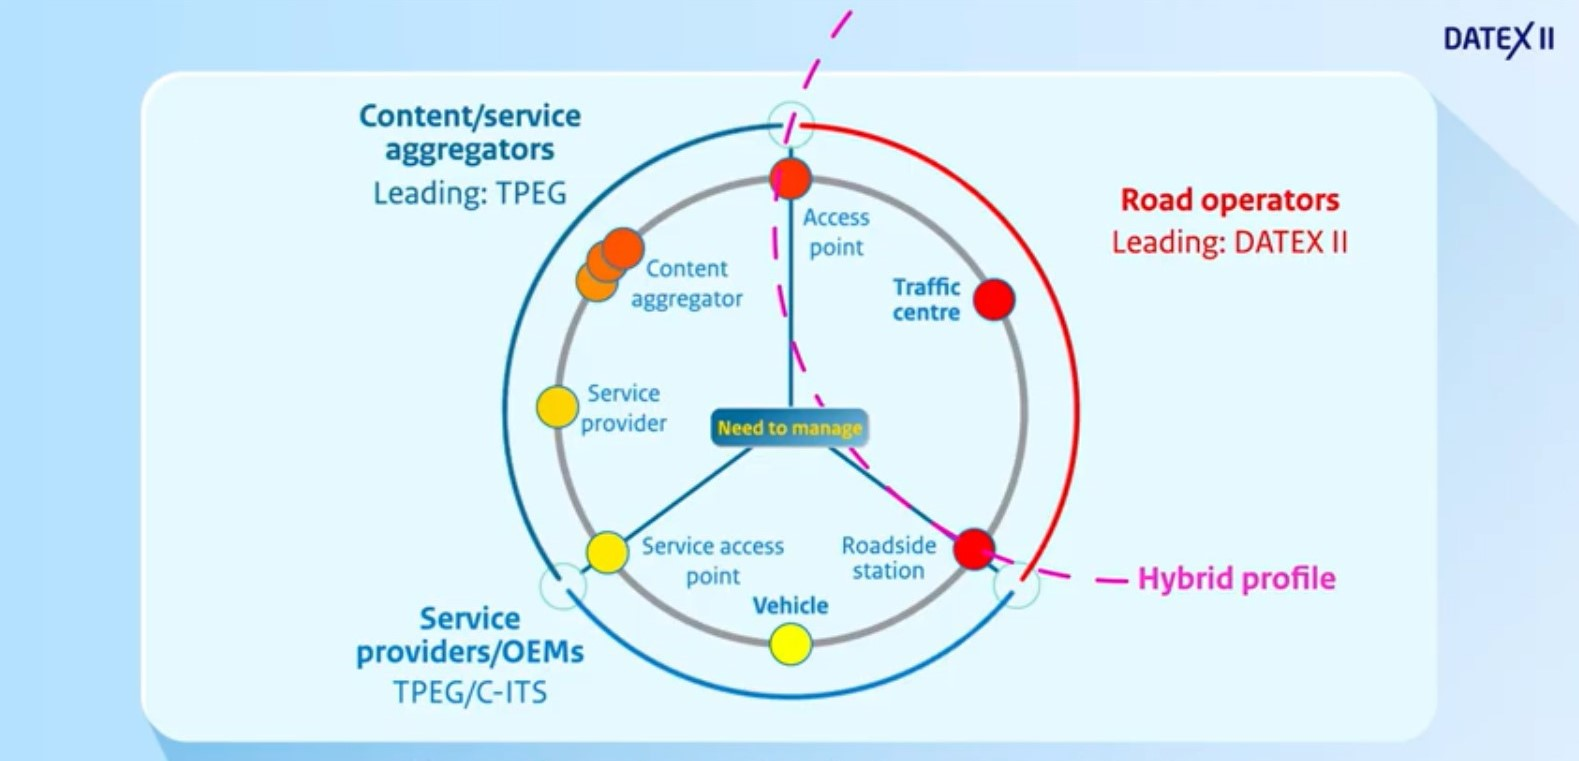
\includegraphics[width=0.8\columnwidth]{images/datexii}
	\end{center}
	\caption{Panoramica del Mondo ITS e le relative sfide tecnologiche}
	\label{fig:datexii}
\end{figure}
\begin{table}
	\begin{center}
		\begin{tabular}{|l|l|}
			\hline
			\textbf{Type} & \textbf{Remarks} \\
			\hline
			\pbox{20cm}{Accidents \\ Obstruction \\ Activities \\} & public events, police operations etc.  \\
			\hline
			\pbox{20cm}{Abnormal Traffic \\ Driving conditions \\ Poor road infrastructure \\ Network Management \\ Sign information \\ Roadside Assistance \\ Car parking information \\ Transit information \\ Service disruption \\} & \pbox{20cm}{Queues \\ Weather, Road surface \\ Closures, Restrictions \\ VMS settings \\ Number of vacant spaces \\ Rail and Ferry connections \\ Motorway service area} \\
			\hline
			\pbox{20cm}{Measured Traffic Data \\ Measured weather/pollution  \\} & \pbox{20cm}{Travel times, Flow data \\ Wind, precipitation, visibility, air quality} \\
			\hline
			\pbox{20cm}{Traffic View  \\} & \pbox{20cm}{Combination of event informations and URLs for CCTV cameras} \\
			\hline
		\end{tabular}
		\caption{Le metodologie di comunicazione \cite{famous:paper_datexii_research}}
		\label{tabel:datexii_data}
	\end{center}
\end{table}
Lo Standard DATEX II non è stato pensato per fornire delle rigide specifiche di comunicazione ma piuttosto come un Protocollo che ammettesse una certa libertà di scelta e che fosse in grado di evolversi per consentire, in futuro, lo scambio di informazioni aggiuntive.\\
Il dominio di dati che possono essere scambiati attraverso DATEX II riguarda tutti i dati relativi al trffico ed alle informazioni sul viaggio per strade urbane ed inter-urbane. Spaziando tra eventi legati al trffico come incidenti e lavori stradali ad eventi legati al flusso di traffico come permanenza sulle strade e durata del viaggio. \\
Risultano quindi evidenti le motivazioni che hanno portato alla scelta dello standard DATEX II nella progettazione del prototipo ideato in \autoref{sec:general_idea}. Rispetto ad altri protocolli di comunicazione, infatti, DATEX II presenta delle caratteristiche che ben si adattano allo scopo:
\begin{enumerate}
	\item Sviluppato, Supportato ed Utilizzato dalla Comunità Europea
	\item Progettato per lo scambio di dati relativi al traffico
	\item Supporta lo scambio dati tra dispositivi eterogenei
	\item Indipendente dalla tecnologia utilizzata per lo scambio dati
	\item Flessibile per adattarsi a nuove necessità e dati da scambiare
	\item Geo-Referenzia i dati scambiati tra i vari dispositivi
	\item Documentazione completa per gli sviluppatori che vogliano integrare il protocollo nelle loro applicazioni
	\item Documentazione completa per gli sviluppatori che vogliano ampliare il protocollo in funzione di nuove necessità
\end{enumerate}
Progettando quindi il sistema della \autoref{sec:general_idea} in modo che supporti il protocollo DATEX II, si fa in modo che il sistema possa essere aperto a ricevere non solo i dati provenienti da altri smartphone o tablet sui quali è installato lo stesso sistema, ma anche da Centri per il controllo del traffico, infrastrutture stradali e centri di informazione su tutta la rete stradale Europea, avendo così a disposizione un più ampio data-source sulla base del quale effettuare previsioni, analisi ed inviare comunicazioni agli utenti.

\subsection{DATEX II Data Model}
\label{sec:datexii_data_model}
Il principale vantaggio del Protocollo DATEX II è la sua flessibilità che lo rende a prova di futuro. Questa caratteristica viene fornita allo standard da un ricco ed ampiamente sviluppato modello dei dati in formato UML (Unified Modeling Language). Questo consente allo Standard DATEX II di avere un modello dei dati che sia indipendente dalle sue implementazioni e che quindi possa essere mappato diversamente in diverse implementazioni.
Attualmente, questo modello dei dati è mappato in informazioni codificate attraverso XML (eXtensible Markup Language) con la creazione di un XML schema. XML e XML schema sono tra i sistemi per la definizione dei modelli di dati più ampiamente utilizzati. Questa scelta garantisce che l'interfaccia DATEX II sia facilmente integrabile in quante più implementazioni ed applicazioni possibili.\\
In più, DATEX II implementa un alto livello di flessibilità attraverso una opzione di estensibilità del modello dei dati. Questo consente ad utenti singoli di scambiare dati attraverso il modello dei dati DATEX II, ma che sia stato adattato alle loro particolari necessità e preferenze, rimanendo comunque conforme allo standard DATEX II. Questo viene reso possibile offrendo agli utenti la possibilità di ampliare il modello dei dati di DATEX II, seguendo una definita procedura, in modo che si mantenga l'interoperabilità con altri dipositivi e centri di controllo per il traffico che utilizzino una qualsiasi altra implementazione conforme a DATEX II. \cite{famous:paper_datexii_research}\\
Lo sviluppo do DATEX II si è focalizzato sulla creazione di un documento di riferimento nel quale viene posta particolare enfasi alla distinzione tra Data (contenuto) e Meccanismo di Scambio. La descrizione tecnica fornisce una chiara distinzione tra Platform Independent Modelling (PIM) e Platform Specific Modelling (PSM). PIM si riferisce al dominio dei dati scambiati relativi al traffico mentre PSM si riferisce alle specifiche informazioni scambiate ed alla tecnologia di comunicazione utilizzata.
Questa separazione tra i due domini produce una migliore comprensione dello standard rendendolo più facile da applicare.

\subsubsection{Level A - Data Model}
DATEX II viene sviluppato a valle di un periodo di studio ed osservazione sul tipo e numero di dati che sono scambiati dai dispositivi IoT nella Comunità Europea. Risultato di questa osservazione è il modello dei dati in formato UML di DATEX II anche noto con il termine "Level A Data Model". Sebbene ampiamente completo e documentato, potrebbero ancora esserci delle situazioni nelle quali l'interfaccia dati richiesta da un particolare utente possa non essere presente nel Data Dictionary di DATEX II in quanto, ad esempio, sono dati riferiti ad un contesto nazionale o locale.\\
In questo caso, questi utenti sono in  grado di fornire una estensione al modello che includa i concetti mancanti, nota anche come "Level B Extension Model". Agli utenti viene quindi data la possibilità di aggiungere una limitata estensione al diagramma UML, seguendo predefinite istruzioni. Queste estensioni (Level B) devono comunque mantenere l'interoperabilità con lo standard DATEX II in modo che altri dispositivi che siano compatibili con DATEX II (ad esempio con il Level A), possano ancora mantenere una interoperabilità e che cioè siano in grado di processare i dati (o Publications) provenienti da un dispositivo che implementi un modello dei dati personalizzato (ad esempio di Level B), senza essere ovviamente in grado di processare i dati aggiunti dal particolare client.\\
Soltanto altri client specializzati, che cioè implementano tutto il modello dei dati modificato (di Level B) saranno in grado di processare tutto il contenuto, comprese le estensioni.\\
Lo scopo principale per cui il Level B è progettato riguarda i soli casi in cui uno specifico utente implementi ed utilizzi il modello dei dati di Level A per la maggior parte delle comunicazioni ma che, in alcuni casi, non sia sufficiente a soddisfare le proprie necessità e risulta necessario ampliarlo.\\
Questo tuttavia non comprende il caso nel quale si vogliano definire dei concetti che siano completamente nuovi o completamente fuori dallo scope del Level A. In questo caso, gli utenti che dovessero incorrere in tali necessità hanno ancora la possibilità di ampliare il modello dei dati nel diagramma UML così da avere ancora un certo livello di interoperabilità. Questi modelli così modificati sono chiamati "Level C Extensions". Le implementazioni che forniscano dei dati (o Publications) di Level C non sono generalmente in grado di essere interoparabili con le implementazioni di Level A o Level B.
.
\subsubsection{Level B - Extension Mechanism}
Sebbene il Level A sia già abbastanza ricco ed il suo modello dei dati abbastanza completo, non è escluso che nel tempo possano sorgere delle nuove necessità o applicazioni che vogliano aggiungere nuovi concetti ed attributi al modello esistente. Al fine di rendere il Protocollo DATEX II adatto a sopravvivere alle innvovazioni nel tempo, è stato progettato un meccanismo formale attraverso il quale il modello dei dati di Level A puù essere esteso. E' necessario che queste nuove applicazioni che estendono il Level A, chiamate Level B, mantengano una compatibilità con il DATEX II nella sua versione base (Level A). Questo consente alle nuove implementazioni dello standard che arricchiscano il Level A con l'aggiunta di nuovi concetti o attributi di restare comunque compatibili con lo standard nella sua versione base e quindi di interpretare correttamente le publications.
Fornitori o Client che volessero utilizzare completamente le informazioni definite in queste estensioni al Level A devono invece implementare il modello dei dati definito nell'estensione stessa Level B e non il solo modello base Level A.\\
Presso \url{www.datex2.eu} è disponinbile un processo di registrazione di nuove estensioni di tipo B allo standard DATEX II. Qualora queste estensioni dovessero raggiungere ampio consenso, saranno integrate direttamente nella versione base dello standard.

\subsubsection{Level C - Extensions}
Dopo aver analizzato le possibilità offerte dalle versioni A e B dello standard DATEX II e dalla loro intercompatibilità, alcuni utenti potrebbero ancora ritenere necessario un ampliamento ancora più profondo dello standard con l'aggiunta di nuove ddefinizione e di nuovi scope. Queste modifiche potrebbero anche rivelarsi troppo distanti dal modello dei dati di Level A e quindi non implementabili con una sola estensione del Level A in Level B. Per questo motivo, viene anche sviluppato il concetto di Level C le cui implementazioni sono considerate non conformi allo standard e quindi non interoperabili con i Level A, B. Nonostante questa incompatibilità, le implementazionid i Level C devono quantomeno utilizzare le regole di modelling e protocolli di scambio dati che siano comuni a DATEX II.
Questo potrebbe consentire in futuro uno scambio di idee e portare alla creazione di un modello dei dati unificato.

\subsubsection{Data Dictionary}
Lo standard DATEX fornisce le definizioni di quelli che sono i concetti e gli attributi utilizzati nel modello dei dati in modo da aiutare gli sviluppatori nell'utilizzo ed implementazione dello Standard. Queste definizioni sono raccolte in un diagramma UML per gli addetti ai lavori ed in un file Excel che documenti tutte le definizioni in una forma più comprensibile. In questo modo, è possibile istantaneamente valutare se lo standard comprenda già tutti gli attributi necessari alla particolare istanza o se sia necessario aggiungerne di nuovi.

\subsection{XML Schema}
Il formato XML sta vedendo una notevola crescita del suo utilizzo per lo scambio di informazioni. Una componente fondamentale di questo approccio sono gli XML Schemas. Basandosi su un modello dei dati e su un dizionario dei dati, gli XML Schemas sono progettati per adattarsi ad una particolare area applicativa. Questi schemi sono degli strumenti per capire il contenuto dei dati che sono scambiati.\\
Il modello UML viene inizialmente esportato in un file XMI ed in seguito, attraverso un tool di conversione, viene trasformato in un XML Schemas.
Questi XML Schemas sono utilizzati per lo sviluppo sofwtare. XMI (XML Metadata Interchange) è invece uno standard OMG per lo scambio di metadati in formato XML. L'uso più comune che se ne fa di XMI è proprio quello di interscambio di modelli UML.
\begin{figure}
	\begin{center}
		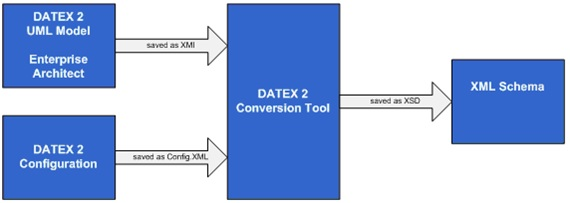
\includegraphics[width=0.8\columnwidth]{images/datexii_xml}
	\end{center}
	\caption{Workflow di un processo di conversione automatico}
	\label{fig:datexii_xml}
\end{figure}

\subsection{Exchange Mechanisms}
Ci si focalizza ora su quali metodologie sono supportate dal protocollo DATEX II per lo scambio dei dati tra i diversi dispositivi che partecipano alla piattaforma. \\
DATEX II offre metodologie di push e pull per lo scambio di informazioni. \\
La modalità \textbf{push} consente al fornitore di inviare le informazioni al client. Questa operazione può essere effettuata periodicamente ad intervalli di tempo regolari oppure all'occorrenza quando il fornitore dovesse ritenerlo opportuno.\\
La modalità \textbf{pull} consente al client di richiedere dati ad un fornitore.\\
Una descrizione di alto livello di come avvenga la comunicazione tra fornitore e consumatore dei dati, senza considerare i dettagli tecnici, può essere sintetizzata in tre operazioni principali:
\begin{enumerate}
	\item \textbf{Publisher Push on Occurrence: } La comunicazione e l'invio dei dati viene cominciata dal publisher ogni volta che i dati cambiano
	\item \textbf{Publisher Push Periodic: } La comunicazione e l'invio dei dati viene cominciata dal publisher ad intervalli di tempo regolari
	\item \textbf{Client Pull: } La comunicazione viene cominciata dal Client che si aspetta l'invio dei dati richiesti come risposta dal Publisher
\end{enumerate}
Le metodologie di comunicazione viste finora possono essere sia online che offline. Nel Platform Specific Modelling (PSM), la sezione relativa allo scambio dei dati è stata progettata per essere indipendente dal contenuto che viene scambiato, ovvero dal payload. In questo modo, le informazioni relative allo scambio dei dati possono essere studiate indipendentemente dal modello dei dati in formato UML di DATEX II, garantendo così la separazione dei due campi.\\
Questa separazione logica ed implementativa, non solo rende più facile la comprensione e l'applicazione del protocollo stesso, ma rende anche possibile riutilizzare una delle due sezioni qualora l'altra dovesse cambiare ed evolversi nel tempo per adattarsi a nuove necessità. Ad esempio, potrà variare nel tempo il modello dei dati dello standard DATEX II perchè potrebbero essere proposte delle nuove estensioni dello standard, tuttavia, non è necessario che vari anche il meccanismo di scambio dati in quanto indipendente dal payload.

\subsection{Exchanged Data}
Prima di analizzare nel dettaglio come sia fatto il diagramma UML relativo allo Standard DATEX II ed implementarlo nel sistema che prototiperà lidea della \autoref{sec:general_idea}, si analizzino più nel dettaglio i dati relativi al traffico che sono supportati dallo standard.\\
Questi dati che vengono scambiati, sono composti da elementi base che sono disponibili all'interno di una pubblicazione o alternativamente potremmo dire che tra i dispositivi viene scambiata una publication composta da elementi o attributi base.

\subsubsection{Elementi Base}
Una Publication in DATEX II è composta da elementi base che possiamo raggruppare in macro-categorie: 
\begin{enumerate}
	\item Eventi relativi a condizioni stradali e traffico ("Traffic Elements")
	\item Azioni dell'Operatore
	\item Incidenti
	\item Dati misurati o elaborati (tempo di viaggio, velocità del traffico stimata, intensità del traffico stimata, rilevazioni metereologiche, ...)
	\item Messaggi mostrati sui Variable Message Signs (VMS)
	\item Informazioni di Servizio (assenza di corsie di emergenza, ritardi su treni, ...)
\end{enumerate}
In più, sono anche presenti elementi come: Zone di Posteggio, Posizioni dei pannelli VMS e Posizioni dei siti di misura. 
Queste infromazioni, sebbene non siano dei dati elementari, sono comunque necessarie al Client al fine di comprendere ed utilizzare correttamente le informazioni degli elementi base.

\subsubsection{Eventi relativi a condizioni stradali e traffico}
Questi eventi riguardano tutti situazioni che non sono inizializzate da un operatore del traffico ma che lo obbligano ad intraprendere una decisione su come affrontare l'evento. Possono essere classificati in:
\begin{itemize}
	\item Traffico Anormale (lunghe code, rallentamenti)
	\item Incidenti
	\item Attività (eventi pubblici, disturbi al normale funzionamento)
	\item Condizioni Stradali. Possono essere o meno legate a condizion atmosferiche o all'ambiente
	\item Ostruzioni
	\begin{itemize}
		\item presenza di animali
		\item presenza di veicoli in panne
		\item ostruzioni dovute dall'ambiente (alberi)
		\item ostruzioni dovute a infrastrutture (caduta di cavi)
		\item ostruzioni dovute a persone
	\end{itemize}
	\item Incidenti ad infrastrutture o sistemi stradali (VMS guasti)
\end{itemize}

\subsubsection{Azioni dell'Operatore}
Riguardano eventi che sono inizializzati da un operatore del traffico e possono essere classificati in:
\begin{itemize}
	\item Manutenzione (chiusura di strade, traffico alternato)
	\item Lavori stradali (limiti temporanei, deviazioni)
	\item Assistenza a bordo strada
\end{itemize}

\subsubsection{Incidenti}
Questa sezione contiene in particolar modo gli eventi relativi alla disponibilità di corsie, rallentamenti ed eventuali deviazioni.

\subsubsection{Dati Misurati o Elaborati}
Questo set di dati può essere derivato da input diretti di stazioni per il traffico o strumentazione di uno specifico sito di misura, i quali dati possono essere ricevuti periodicamente o possono essere inviati in funzione delle condizioni di traffico in una specifica località.
\begin{itemize}
	\item Valori di Traffico misurati
	\begin{itemize}
		\item flusso
		\item velocità
		\item progresso
		\item concentrazione dei veicoli in coda		
	\end{itemize}
	\item Stato del traffico
	\begin{itemize}
		\item flusso libero, intenso, congestionato, sconosciuto
	\end{itemize}
	\item Tempo di viaggio
	\begin{itemize}
		\item tempo stimato
		\item tempo di viaggio nominale atteso
	\end{itemize}
	\item Condizioni Atmosferiche
	\begin{itemize}
		\item precipitazioni, vento, temperatura, inquinamento, condizioni del manto stradale e visibilità.
		\item previsioni metereologiche
	\end{itemize}
\end{itemize}

\subsubsection{Messaggi mostrati sui VMS}
Questo set di dati include diversi messaggi che possono essere mostrati sui differenti VMS (Variable Message Signs) in funzione della tecnologia che utilizzano, immagini e testo. Possono anche includere informazioni sulla posizione dei dispositivi VMS e sul loro status.

\subsubsection{Informazioni di Servizio}
Riguardano informazioni su un servizio che potrebbe influenzare il comportamento dei guidatori e quindi le caratteristiche del traffico.
\begin{itemize}
	\item  Informazioni sul Transito dei veicoli
	\begin{itemize}
		\item informazioni circa altri mezzi di trasporto (treni, tram, voli)
	\end{itemize}
	\item Indisponibilità di servizi (aree di sosta chiuse, aree di rifornimento chiuse)
	\item Indisponibilità di servizi stradali (chiamate di emergenza fuori uso)
\end{itemize}

\subsection{Publication di Elementi Base}
\label{sec:publication_base_element}
Gli elementi base mostrati in precedenza, possono essere scambiati individualmente tra dispositivi che implementano lo standard DATEX II o possono anche essere scambiati in gruppi di elementi. Questi scambi di gruppi di elementi base prendono il nome di Publication e, in funzione dei dati trasmessi, possono esserci cinque tipi fondamentali di Publication:
\begin{enumerate}
	\item \textbf{Situation Publication: } Usata per Elementi legati al traffico, azioni dell'operatore, incidenti o informazioni di servizio
	\item \textbf{Elaborated Data Publication: } Usata per lo stato del traffico, per i tempi di viaggio e per valori misurati di traffico e condizioni atmosferiche
	\item \textbf{Measured Data Publication: } Usata per Misure del traffico e rilevamenti atmosferici, stato del traffico e tempo di viaggio
	\item \textbf{Parking Publication: } Usata per le informazioni su parcheggi ed aree di sosta
	\item \textbf{VMS Publication: } Usata per i messaggi da mostrare sui VMS e sulle informazioni relative agli VMS.
\end{enumerate}

\subsection{Utilizzo del DATEX II Data Model}
Nelle sezioni precedenti, servendosi della documentazione ufficiale messa a disposizione dallo Standard DATEX (\url{https://datex2.eu/}), si sono evidenziati i vantaggi nell'adozione del protocollo ed anche le sue peculiarità implementative. Data la flessibilità offerta dal protocollo, risulta necessaria ora una fase di analisi su quelle che siano le caratteristiche del protocollo che è necessario implementare all'interno del sistema. Già da una prima analisi sull'idea del prototipo da realizzare, risulta subito evidente che sia superfluo implementare il protocollo DATEX II nella sua interezza in quanto, non tutte le sue componenti saranno necessarie al sistema. \\
Il punto di partenza di questa analisi è quello di adottare il Processo Unificato (UP) con il quale produrre la documentazione necessaria allo sviluppo del software relativo al sistema che si vuole implementare definito nella \autoref{sec:general_idea}. A tal proposito, è bene introdurre brevemente il Processo Unificato ed in generale gli strumenti messi a disposizione dall'Ingegneria del Software che saranno utilizzati nei capitoli seguenti.

\subsubsection{Il Processo Unificato}
Il Processo Unificato (UP) è uno dei modelli messi a disposizione dall'Ingegneria del Software che fornisce una sequenza di fasi da seguire per la progettazione e realizzazione di Software dalle grandi dimensioni. Il Processo Unificato e gli altri modelli per lo sviluppo di Software definiscono la lista di operazioni da seguire al fine di ottenere un prodotto software composto dal suo eseguibile, più la documentazione ad esso associato. Risulta infatti necessario, per software dalle grosse dimensioni, documentare ogni singola fase dello sviluppo, comprese quelle di progettazione.\\
Nello sviluppo di questo particolare sistema, la scelta è ricaduta sul Processo Unificato in quanto questo modello sia particolarmente flessibile ed adatto alla modellazione visuale attraverso l'Unified Modelling Language (UML) che è la stessa tipologia di modellazione utilizzata dallo standard DATEX II. In questo modo, sarà più semplice integrare il Software che si intende sviluppare in questo lavoro di tesi con il Protocollo DATEX II.\\
Il Processo Unificato si compone di diverse fasi, nelle quali ci si focalizza su vari aspetti del processo software e tra le quali fasi si può ciclicamente iterare per implementare nuove funzionalità del Software:\\
\begin{enumerate}
	\item \textbf{Ideazione: } Fornisce una visione approsimativa del progetto. Stime sul progetto di carattere economico e relative alle tempistiche.
	\item \textbf{Elaborazione: } Viene raffinata la visione del progetto, vengono identificati la maggior parte dei requisiti e sono realizzate delle stime più realistiche del progetto.
	\item \textbf{Costruzione: } Fase di implementazione iterativa degli elementi rimanenti e preparazione al rilascio.
	\item \textbf{Transizione: } Beta test e Rilascio agli utenti.
\end{enumerate}
\begin{figure}
	\begin{center}
		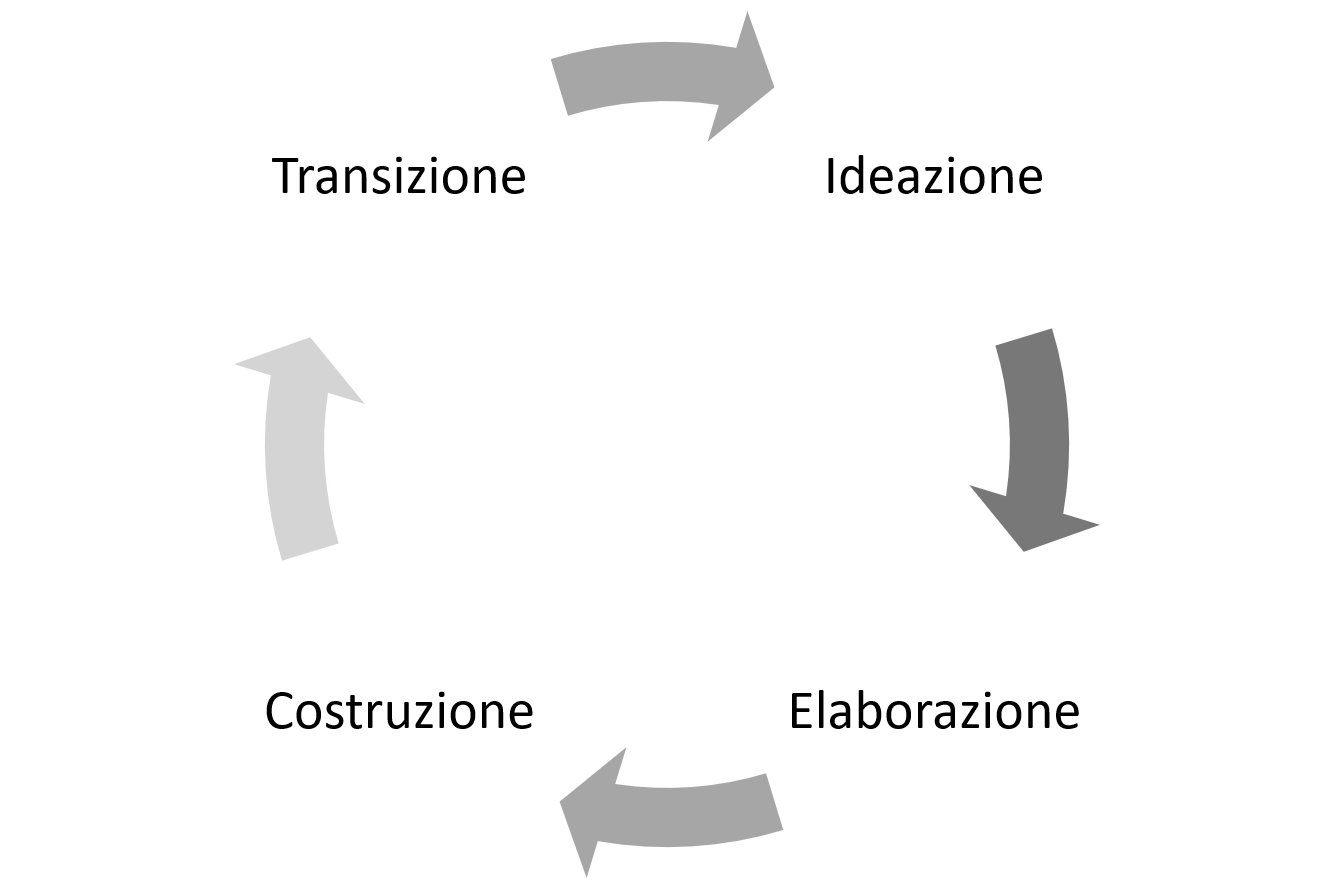
\includegraphics[width=0.5\columnwidth]{images/up}
	\end{center}
	\caption{Fasi del Processo Unificato}
	\label{fig:up}
\end{figure}
Nella fattispecie, si produrrà in questo lavoro di tesi una parte della documentazione prevista dal Processo Unificato per la realizzazione del Software che prototiperà l'idea descritta nella \autoref{sec:general_idea} che sarà di supporto alla progettazione e sviluppo del Software ed alla sua comprensione ed il suo adammento a nuove applicazioni. \cite{book:slide_Nocera}, \cite{book:software_engineering}

\subsubsection{Requisiti Funzionali}
Uno dei documenti che è necessario produrre se si vuole intraprende l'utilizzo del Processo Unificato è l'Analisi dei Requisiti Funzionali. I Requisiti di un Software possono infatti essere suddivisi in:
\begin{itemize}
	\item \textbf{Funzionali: }che riguardano cioè le funzionalità che si vuole implementare all'interno di un Software. \textbf{COSA}
	\item \textbf{Non Funzionali: }che riguardano cioè le performances di funzionamento del Software. \textbf{COME}
\end{itemize}
Per avere una panoramica sull'interfaccia del Protocollo DATEX II che dovrà essere implementata nel sistema, si analizzino ora i requisiti funzionali del sistema descritto nella \autoref{sec:general_idea}, che faciliteranno lo sviluppo Software e documentarenno i passi e le scelte progettuali effettuate durante il processo.\\
In accordo con il modello UP, il documento che verrà redatto in questa sezione non si intende completo ma è solo una prima visione generale del progetto. 
\begin{longtable}{|m{2cm}|m{12cm}|}
			\hline
			\textbf{Requisito} & \textbf{Descizione} \\
			\hline
			\textbf{R1} &   Il sistema dovrà essere implementato su smartphone e tablet Android, garantendo un supporto anche alle versioni pregresse del sistema operativo \\
			\hline
			\textbf{R2} &   Il sistema dovrà richiedere l'accesso alle letture dei sensori ed alle relative specifiche tecniche. Si dovrà inoltre poter accedere alla posizione del dispositivo ed alla rete Internet per la comunicazione con API esterne e con il Middleware. \\
			\hline
			\textbf{R3} &   Ove necessario, il sistema deve rielaborare le letture provenienti dai sensori per eseguire un filtraggio. \\
			\hline
			\textbf{R4} &   Il sistema deve essere in grado di supportare le letture provenienti da tutti i sensori attualmente integrati negli smartphone. \\
			\hline
			\textbf{R5} &   Il sistema deve offrire un metodo rapido ed efficiente per l'aggiunta di nuovi sensori per le future evoluzioni degli smartphone. \\
			\hline
			\textbf{R6} &   Il sistema dovrà verificare le specifiche tecniche di tutti i sensori integrati nel dispositivo ed utilizzare le letture dei soli ritenuti affidabili, accurati e conformi alle necessità dell'algoritmo. \\
			\hline
			\textbf{R7} &   Deve essere data la possibilità a coloro che usano il sistema di selezionare le letture dei sensori che si intende condividere con la piattaforma di Crowdsourcing.  \\
			\hline
			\textbf{R8} &   Deve essere data la possibilità a coloro che usano il sistema di inviare le letture dei sensori che sono stati selezionati manualmente.  \\
			\hline
			\textbf{R9} &   Deve essere data la possibilità a coloro che usano il sistema di segnalare l'occorrenza di particolari eventi lungo la rete stradale (incidenti, ostruzioni, rallentamenti, condizioni climatiche).  \\
			\hline
			\textbf{R10} &   All'avviamento, il sistema deve consentire di visualizzare su una mappa gli eventi sul traffico condivisi da altri dispositivi.  \\
			\hline
			\textbf{R11} &   Il sistema deve consentire di selezionare l'area di interesse nella quale visualizzare gli eventi sul traffico condivisi da altri dispositivi.  \\
			\hline
			\textbf{R12} &   Il sistema deve interrogare il Datababase all'interno del quale sono salvati tutti gli eventi per recuperare quelli necessari.  \\
			\hline
			\textbf{R13} &   Deve essere implementato un Database che contenga le segnalazioni sul traffico inviate dai vari dispositivi in maniera geo-referenziata.  \\
			\hline
			\textbf{R14} &   Il Database deve consentire l'elaborazione di query geo-referenziate da parte dell'utenza.  \\
			\hline
			\textbf{R15} &   Il Database deve essere progettato per ottimizzare la risposta alle query geo-referenziate.  \\
			\hline
			\textbf{R16} &   Il sistema deve prevedere l'utilizzo di un Middleware IoT che riceva i dati da smartphone e possa condividerli con dei Database per future analisi di dati e query degli stessi.  \\
			\hline
			\textbf{R17} &   Il sistema deve stabilire una connsessione di tipo MQTT o HTTP con un Middleware per la raccolta dei dati.  \\
			\hline
			\textbf{R18} &   Il sistema deve stabilire una comunicazione di tipo publish/subscriber tra dispositivi Smartphone e Middleware IoT.  \\
			\hline
			\textbf{R19} &   Una volta stabilita la comunicazione con il Middleware, il dispositivo Android deve inviare le letture dei sensori di cui è dotato a cadenza periodica oppure al click di un bottone da parte dell'utente.  \\
			\hline
			\textbf{R20} &   Il sistema dovrà prevedere l'implementazione del protocollo DATEX II per le sole componenti ritenute necessarie.  \\
			\hline
			\textbf{R21} &   Il sistema dovrà formattare ed interpretare i dati in formato XML in accordo con lo standard DATEX II.  \\
			\hline
			\textbf{R22} &   Il sistema dovrà inviare i dati formattati secondo il protocollo DATEX II in formato JSON al middleware IoT.  \\
			\hline
			\textbf{R23} &   Il sistema dovrà consentire la registrazione di un nuovo utente attraverso i suoi dati personali ed associare di conseguenza un token al particolare utente per l'accesso alle prestazioni di API esterne, del Middleware IoT e dell'accesso al Database.  \\
			\hline
		\caption{Analisi dei requisiti funzionali seguendo il modello di sviluppo UP}
		\label{tabel:requisiti_software}
\end{longtable}

\subsubsection{Diagramma delle Classi}
I requisiti visti nella sezione precedente vanno ora confrontati con ciò che viene offerto dallo standard DATEX II in modo da implementare la sola interfaccia necessaria a soddisfarne i requisiti identificati del sistema.
La Commissione responsabile dello sviluppo dell'interfaccia DATEX II ha messo a disposizione il modello delle classi implementato nello standard al quale fare riferimento per le implementazioni di DATEX II. \url{http://d2docs.ndwcloud.nu/_static/umlmodel/v3.0/index.htm}\\
Il Diagramma delle Classi qui presentato è un altro documento previsto dal modello di sviluppo del Processo Unificato per la documentazione dello sviluppo software. In questo documento, sono contenute le classi e le relazioni tra di esse e serve ad illustrare la struttura del software. Tale documento, tuttavia, serve soltanto ad offrire una panoramica statica delle classi che compongono il Software, senza considerare cioè le singole implementazioni delle stesse. \\
Si intende pertanto in questa sezione, analizzando il diagramma delle classi dello standard DATEX II, implementare il diagramma delle classi (o una parte di esso) del sistema che implementi lo standard per adempiere ai requisiti di \autoref{tabel:requisiti_software}.\\
Essendo la definizione di un protocollo di comunicazione DATEX II definisce anche il significato di tutto ciò che viene trasmesso all'interno del Payload di un pacchetto scambiato tra due dispositivi che partecipano alla comunicazione. La definizione del payload \autoref{fig:datexii_publication_detailed}, può estendere a sua volta anche le definizioni di nuove classi o attributi \autoref{fig:datexii_publication}, purchè rispettino particolari vincoli come indicato nella \autoref{sec:datexii_data_model}
\begin{figure}
	\begin{center}
		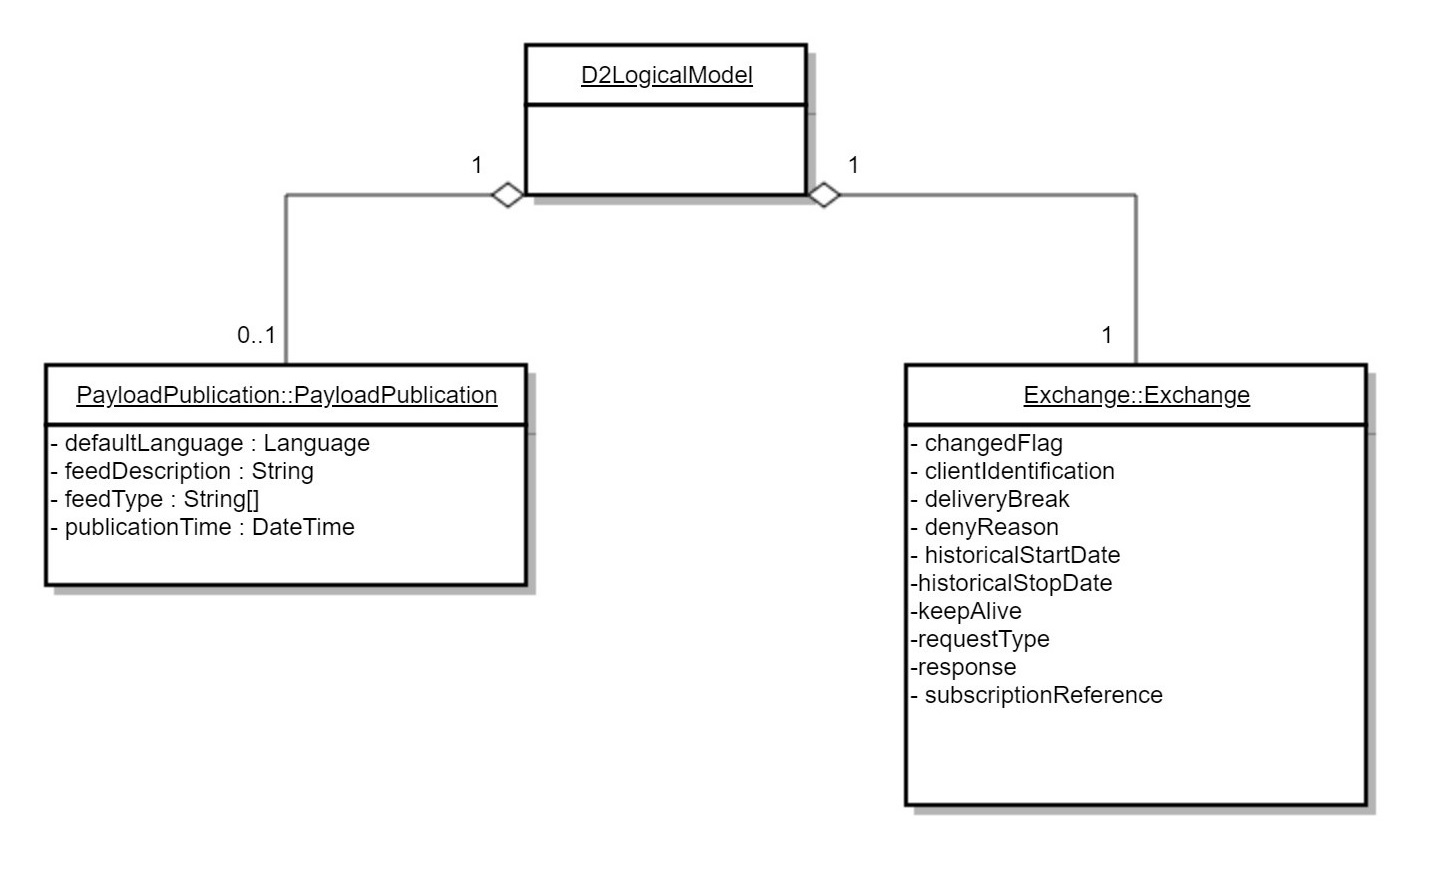
\includegraphics[width=0.6\columnwidth]{images/uml_1}
	\end{center}
	\caption{Distinzione effettuata dallo Standard DATEX II tra metodo di comunicazione (\textit{Exchange}) e formato del Payload (\textit{PayloadPublication})}
	\label{fig:uml_1}
\end{figure}
\begin{figure}
	\begin{center}
		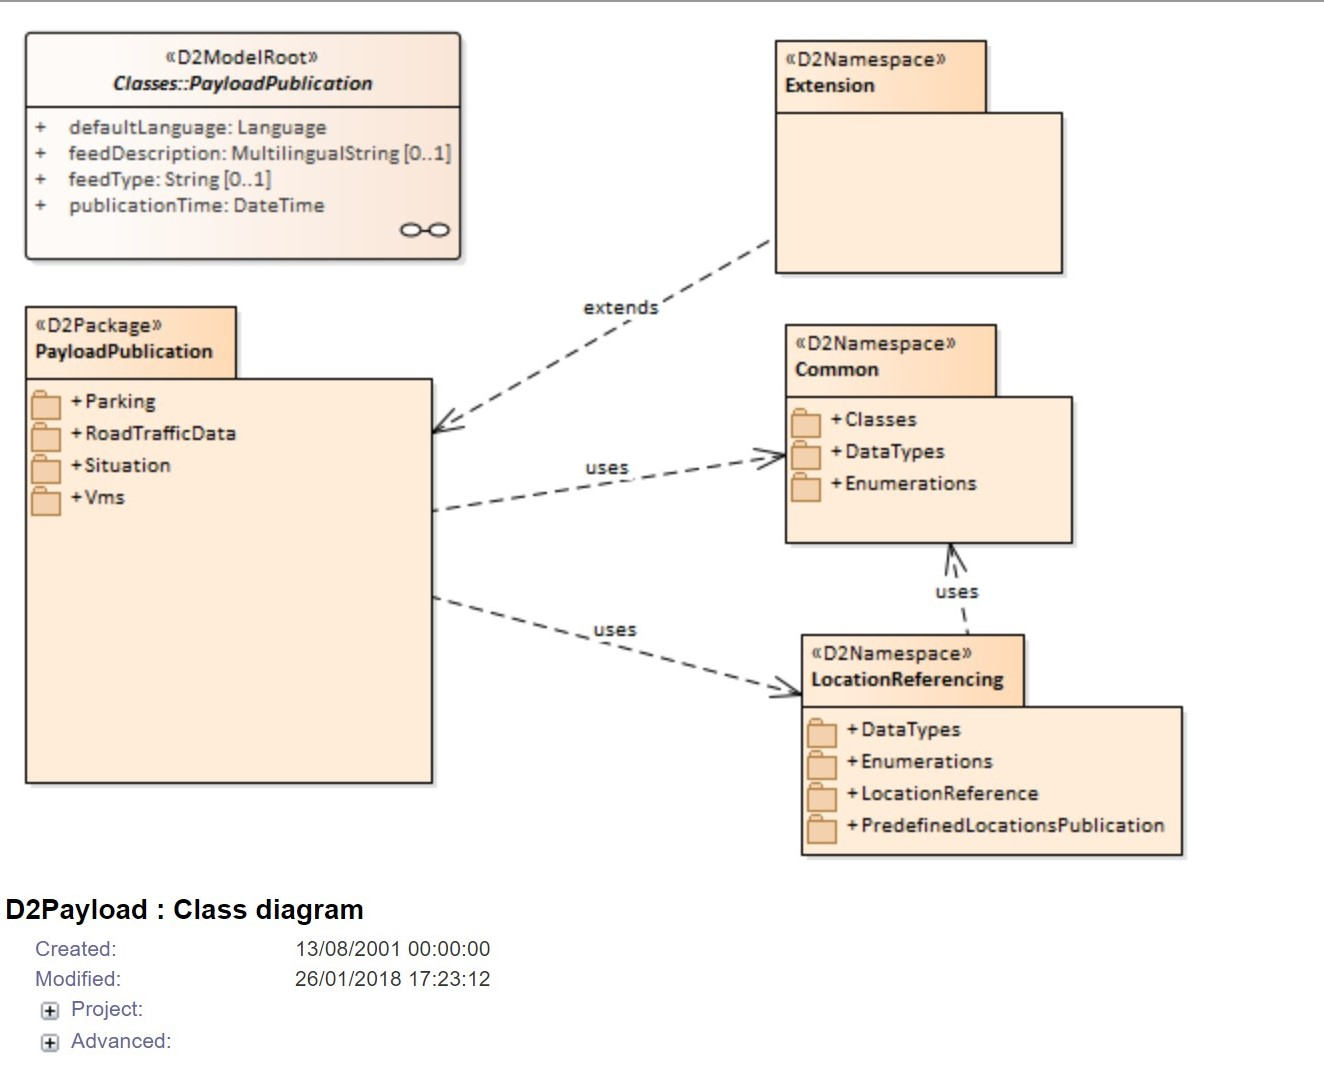
\includegraphics[width=0.6\columnwidth]{images/datexii_publication}
	\end{center}
	\caption{Formato del Payload}
	\label{fig:datexii_publication}
\end{figure}
\begin{figure}
	\begin{center}
		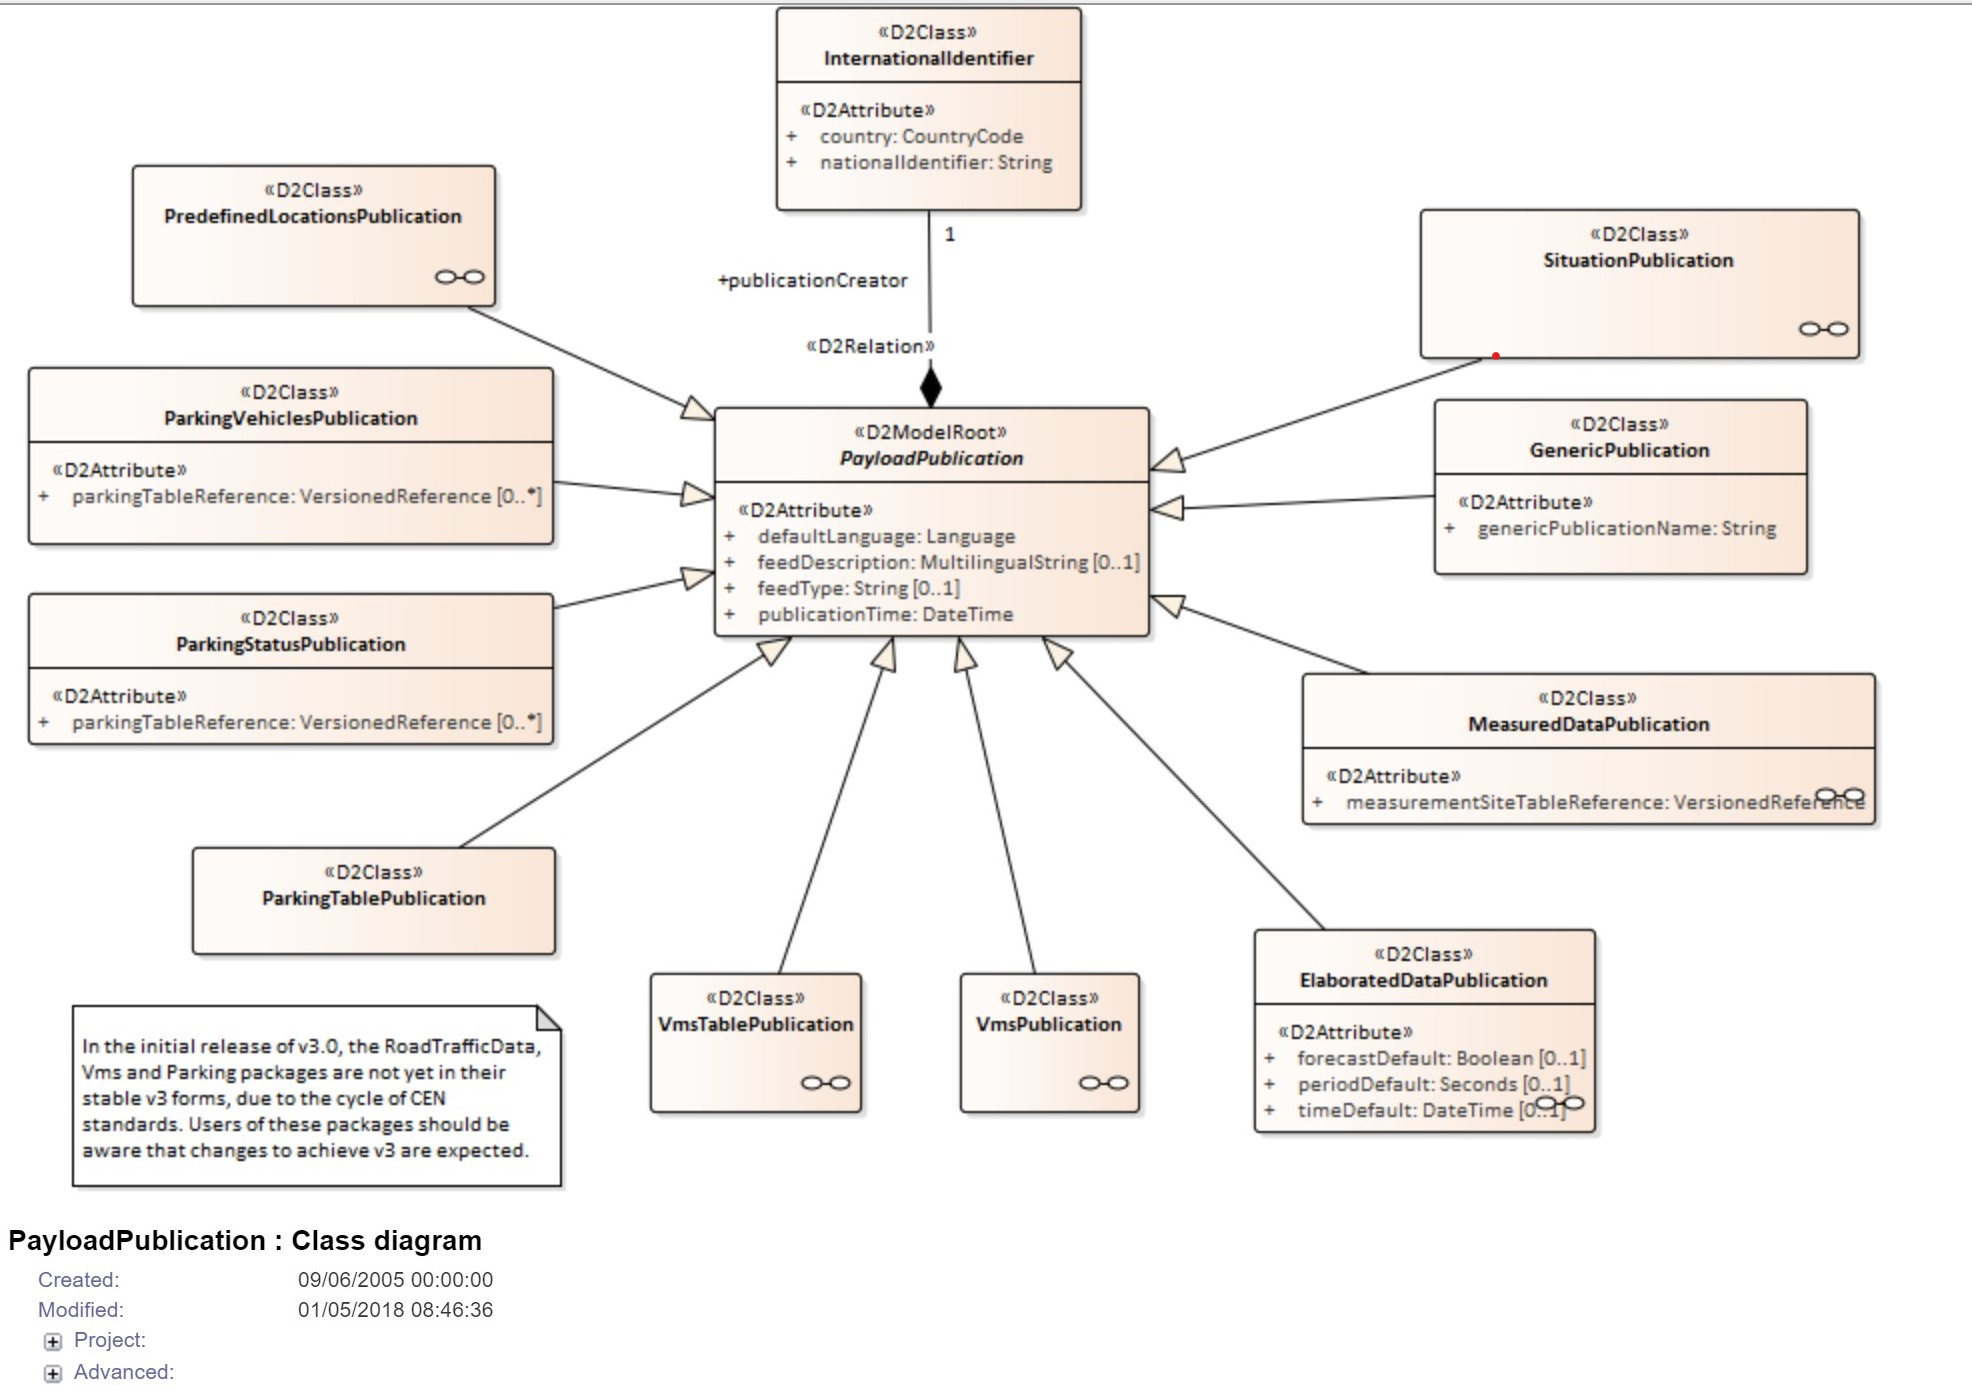
\includegraphics[width=0.75\columnwidth]{images/datexii_publication_detailed}
	\end{center}
	\caption{Formato della Publication}
	\label{fig:datexii_publication_detailed}
\end{figure}
Dalla \autoref{fig:datexii_publication_detailed} è evidente che la classe PayloadPublication sia solo una classe astratta o una interfaccia di classe che viene implementata da altre classi che definiscono tipologie di classi specializzate. Infatti, a conferma di quanto mostrato nella \autoref{sec:publication_base_element}, le Publication possono essere di varie tipologie specializzate a seconda dei dati che trattano.
In funzione dei Requisiti Funzionali in \autoref{tabel:requisiti_software} e dell'idea del sistema nella \autoref{sec:general_idea}, è possibile già filtrare ad alto livello le sole tipologie di publication che è necessario implementare nel sistema.
\begin{figure}
	\begin{center}
		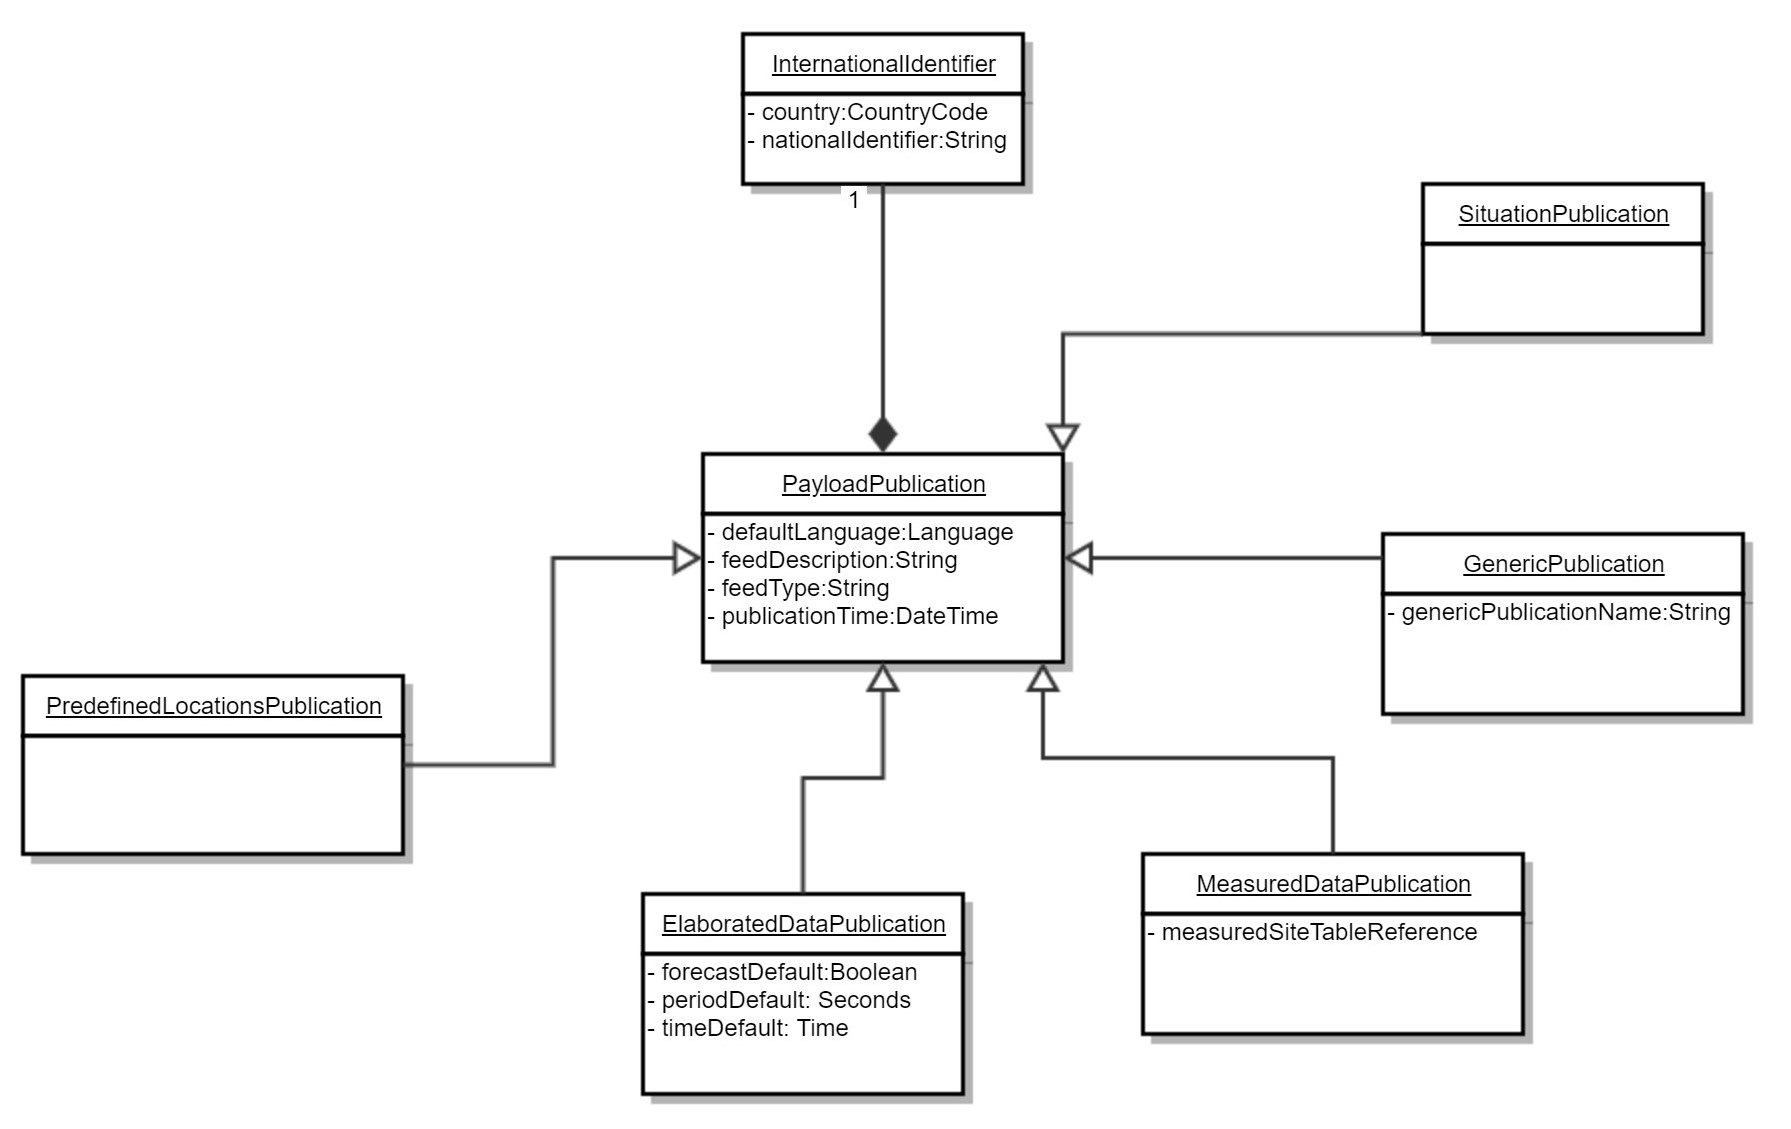
\includegraphics[width=0.8\columnwidth]{images/datexii_publication_implementation}
	\end{center}
	\caption{Implementazione della Publication}
	\label{fig:datexii_publication_implementation}
\end{figure}
Un approccio del tutto simile è stato seguito quindi per tutte le tipologie di Publication che si è ritenuto opportuno implementare. Ovvero, sulla base del diagramma delle classi del protocollo DATEX II, sono state filtrate le sole classi ed attributi necessari a soddisfare i requisiti di \autoref{tabel:requisiti_software}. Il risultato di questo processo è mostrato nell' \autoref{app:a}.

\section{IoT Cloud Platform}
Nella sezione precedente è stato mostrato nei dettagli come procedere all'implementazione del Protocollo DATEX II in un qualsiasi linguaggio di programmazione orientato agli oggetti. In questo modo, si è giunti ad una fase della progettazione del software nella quale i dispositivi che eseguono il sistema, riescono a comunicare tra loro seguendo un Protocollo comune. Sebbene non sia ancora stato definito completamente il contenuto della comunicazione tra due dispositivi (che sarà compito del \autoref{chap:quattro}), è necessario ora progettare una struttura che sia in grado di ricevere questo messaggio, indipendentemente da cosa esso cotenga e di trattarlo opportunamente.\\
E' cioè necessario individuare una Piattaforma Cloud che sia in grado di ricevere i dati provenienti da dispositivi IoT e che sia in grado di conservarli all'interno di opportuni Database, la cui struttura sarà descritta nella \autoref{sec:database}.\\
\begin{figure}
	\begin{center}
		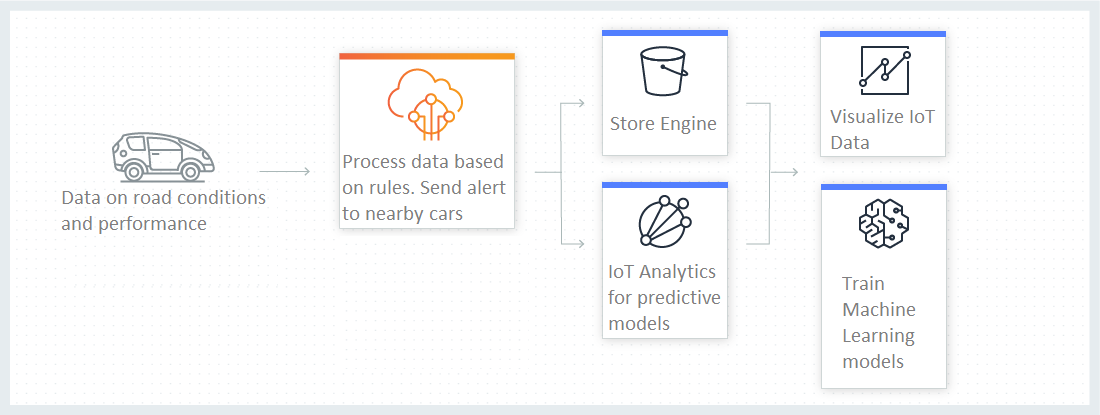
\includegraphics[width=0.9\columnwidth]{images/iot_middleware}
	\end{center}
	\caption{Schema della componente che si vuole implementare in questa sezione vista nel progetto completo}
	\label{fig:iot_middleware}
\end{figure}
Dal momento che il panorama attuale offre numerosi servizi che possano assolvere a questo compito, si valutino ora i requisiti che il Middleware IoT deve avere per l'implementazione del sistema descritto nella \autoref{sec:general_idea} e, sulla base di questi requisiti, si effettuerà un confronto tra le possibili soluzioni.\\
I requisiti mostrati nella \autoref{tabel:requisiti_middleware} vanno ad aggiungersi a quelli elencati nella \autoref{tabel:requisiti_software} concludendo in questo modo la redazione dell' Analisi dei Requisiti prevista nel Processo Unificato.\\\\
\begin{longtable}{|m{2cm}|m{12cm}|}
	\hline
	\textbf{Requisito} & \textbf{Descizione} \\
	\hline
	\textbf{M1} &   Il Middleware IoT dovrà prevedere un sistema per la registrazione di nuovi utenti \\
	\hline
	\textbf{M2} &   Il Middleware IoT dovrà consentire l'accesso ai soli utenti registrati, instaurando con essi una connessione sicura \\
	\hline
	\textbf{M3} &   Il Middleware IoT dovrà consentire di assegnare diversi ruoli a diversi utenti con diverse permission \\
	\hline
	\textbf{M4} &   Il Middleware IoT deve trattare diversamente i dati provenienti da diverse località geografiche \\
	\hline
	\textbf{M5} &   Il Middleware IoT deve stabilire una comunicazione con un database di tipo SQL/NoSQL per il salvataggio dei dati \\
	\hline
	\textbf{M6} &   Il Middleware IoT dovrà  stabilire una comunicazione di tipo publisher/subscriber con uno o più dispositivi IoT\\
	\hline
	\textbf{M7} &   Il Middleware IoT dovrà essere altamente scalabile per supportare un numero sempre crescente di dispositivi \\
	\hline
	\textbf{M8} &   Il Middleware IoT dovrà consentire la comunicazione con sistemi per la visualizzazione ed analisi dei dati \\
	\hline
	\textbf{M9} &   Il Middleware IoT dovrà implementare il protocollo DATEX II \\
	\hline
	\textbf{M10} &   Il Middleware IoT dovrà supportare diversi protocolli per la comunicazione (MQTT, HTTP, AMQP, etc) per garantire la comunicazione con dispositivi eterogenei \\
	\hline
	\caption{Analisi dei requisiti che la IoT Cloud Platform deve supportare}
	\label{tabel:requisiti_middleware}
\end{longtable}
Le piattaforme che sono state individuate come possibili Cloud Platforms adatte allo scopo sono:
\begin{itemize}
	\item \textbf{AWS IoT Core: } \url{https://aws.amazon.com/it/iot-core/}
	\item \textbf{Azure IoT Lab: } \url{https://docs.microsoft.com/en-us/azure/iot-hub/about-iot-hub}
	\item \textbf{FIWARE: } \url{https://www.fiware.org/about-us/}
\end{itemize}
Le soluzioni identificate, non rappresentano assolutamente l'insieme di tutte le soluzioni possibili per le Cloud Platform, ma solo di quelle ritenute più adatte allo scopo della progettazione del sistema.\\
Di seguito viene proposto un confronto tra le diverse soluzioni elencate sulla base dei requisiti di \autoref{tabel:requisiti_middleware}. Le informazioni sulla base delle quali è stato effettuato questo confronto sono state raccolte dai siti Web di ciascuna soluzione e si intendono riferiti alla alla data della seduta di laurea alla quale questo elaborato si riferisce.\\
\begin{table}
	\centering
	\begin{tabular}{|>{\centering\arraybackslash}m{2.5cm}|>{\centering\arraybackslash}m{4cm}|>{\centering\arraybackslash}m{4cm}|>{\centering\arraybackslash}m{4cm}|}
		\hline
		\textbf{Requisito} & \textbf{AWS IoT Core} & \textbf{Azure IoT Lab} & \textbf{Fiware} \\
		\hline
		\textbf{M1} &  \textcolor{green}{\checkmark} &   \textcolor{green}{\checkmark} &   \textcolor{green}{\checkmark} \\
		\hline
		\textbf{M2} &  \textcolor{green}{\checkmark} &   \textcolor{green}{\checkmark} &   \textcolor{green}{\checkmark} \\
		\hline
		\textbf{M3} &  \textcolor{green}{\checkmark} &   \textcolor{green}{\checkmark} &   \textcolor{red}{$\times$} \\
		\hline
		\textbf{M4} &  \textcolor{green}{\checkmark} &   \textcolor{red}{$\times$} &   \textcolor{green}{\checkmark} \\
		\hline
		\textbf{M5} &  \textcolor{green}{\checkmark} &   \textcolor{green}{\checkmark} &   \textcolor{orange}{Not Implemented} \\
		\hline
		\textbf{M6} &  \textcolor{green}{\checkmark} &   \textcolor{green}{\checkmark} &   \textcolor{orange}{Not Implemented} \\
		\hline
		\textbf{M7} &  \textcolor{green}{\checkmark} &   \textcolor{green}{\checkmark} &   \textcolor{green}{\checkmark} \\
		\hline
		\textbf{M8} &  \textcolor{green}{\checkmark} &   \textcolor{green}{\checkmark} &   \textcolor{orange}{Not Implemented} \\
		\hline
		\textbf{M9} &  \textcolor{green}{\checkmark} &   \textcolor{green}{\checkmark} &   \textcolor{green}{\checkmark} \\
		\hline
		\textbf{M10} &  \textcolor{green}{\checkmark} &   \textcolor{green}{\checkmark} &   \textcolor{green}{\checkmark} \\
		\hline
	\end{tabular}	
	\caption{Confronto tra Cloud Platforms}
	\label{tabel:platform_comparison}
\end{table}
Si noti come, la soluzione proposta da Fiware sia particolarmente interessante in quanto offre una piattaforma open source che quindi può essere adattata alle particolari necessità. Tale soluzione, può essere ritenuta infatti molto promettente per quelle compagnie che vogliano progettare su misura la Cloud Platform ed adattarla alle proprie necessità in modo da avere dei migliori rendimenti prestazionali. Infatti, una soluzione personalizzata, potrebbe offrire prestazioni migliori di soluzioni generali come quelle offerte da AWS ed Azure.\\
Tuttavia, per il dominio di questo lavoro di tesi, la soluzione ideale è quella di sfruttare piattaforme cloud generiche per la raccolta dei dati. In questo modo, si godrà di un ecosistema di servizi ampiamente documentato e ben interfacciato. Infatti, ecosistemi come AWS ed Azure offrono diversi servizi e diverse applicazioni anche al di fuori del dominio dell'IoT. Queste possono essere ad esempio relative ad analisi dei dati, raccolta e storaggio dei dati, servizi di autenticazione e piattaforme di calcolo e machine learning. Tutti questi servizi, sono facilmente utilizzabili e possono facilmente comunicare tra di loro scambiandosi in maniera automatica i dati di cui necessitano. In piattaforme open source, invece, è necessario sviluppare ed interfacciare ciacuno di questi servizi, richiedendo di fatto una mole di lavoro estremamente maggiore.\\
Questa scelta è anche da considerarsi adatta per coloro i quali si interfacciano per la prima volta con una piattaforma cloud in quanto numerosi sono i corsi e le documentazioni offerte da AWS ed Azure.\\
Considerato infine che le funzioni offerte da AWS ben soddisfano i requisiti della \autoref{tabel:requisiti_middleware}, si è scelto di utilizzare questa piattaforma come Middleware IoT che si occuperà della raccolta, condivisione e salvataggio dei dati.

\subsection{AWS IoT Core Overview}
\label{sec:iot_core}
Amazon Web Services IoT Core è una piattaforma cloud che consente a dispostivi connessi di interagire tra loro e con altre applicazioni nel cloud. Inoltre, IoT Core, si interfaccia con tutti gli altri servizi offerti da AWS per il cloud computing and analysis. Ad esempio sarà semplice interfacciare i dati raccolti da IoT core con altri servizi quali:
\begin{itemize}
	\item \textbf{Amazon S3} per la memorizzazione dei dati in Database SQL
	\item \textbf{Amazon DynamoDB} per la memorizzazione dei dati in Database NoSQL
	\item \textbf{Amazon Kinesis ed Amazon QuickSight} per la visualizzazione ed analisi dei dati
	\item \textbf{TensorFlow in AWS} per l'elaborazione dei dati raccolti con tecniche di Machine Learning
\end{itemize}
\begin{figure}
	\begin{center}
		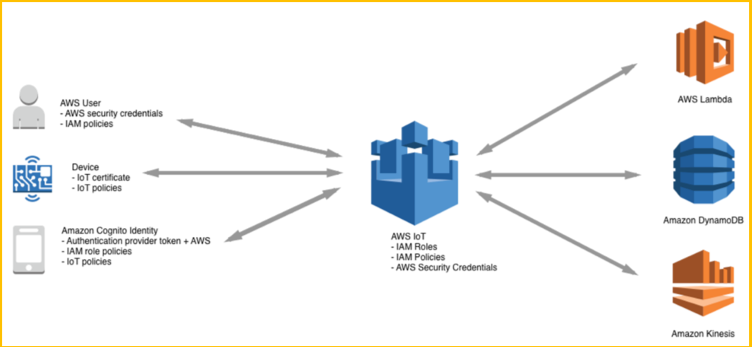
\includegraphics[width=0.9\columnwidth]{images/aws_iot_core}
	\end{center}
	\caption{Capacità di interfacciamento della piattaforma IoT Core con gli altri servizi dell'ecosistema AWS}
	\label{fig:aws_iot_core}
\end{figure}
\begin{figure}
	\begin{center}
		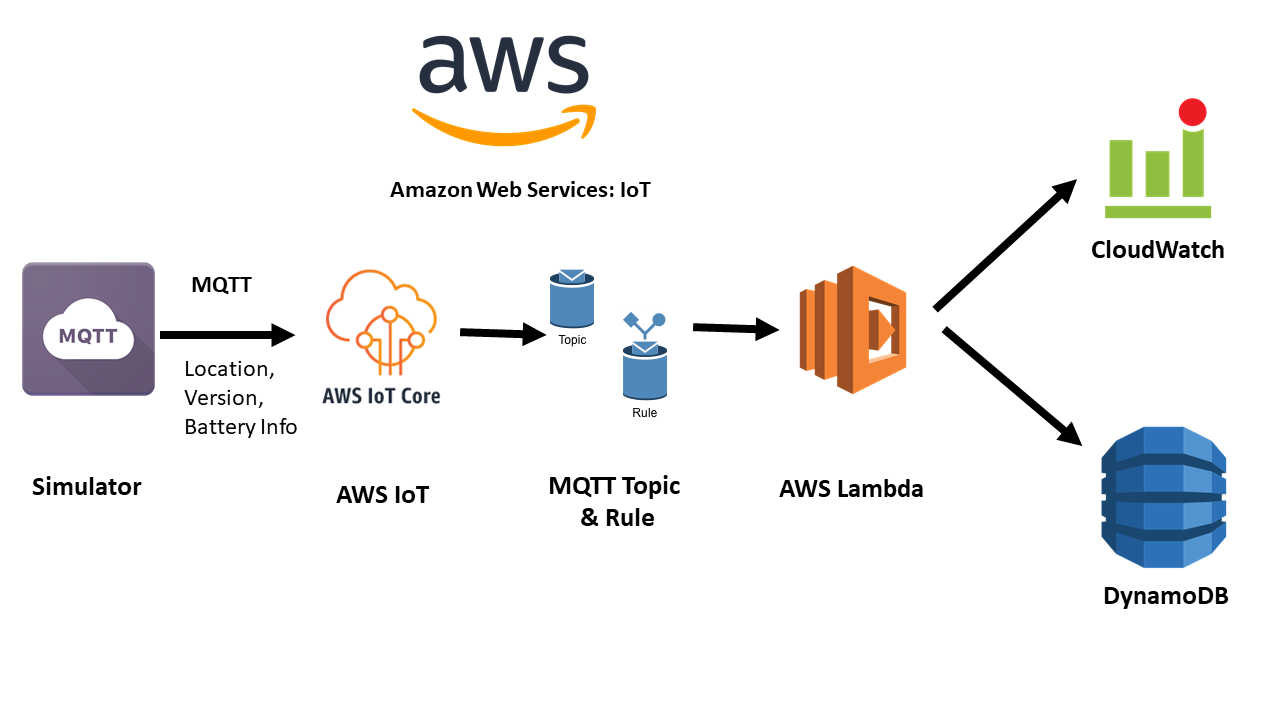
\includegraphics[width=0.9\columnwidth]{images/aws_iot_core_2}
	\end{center}
	\caption{Esempi di utilizzo della piattaforma IoT Core combinata con altri servizi dell'ecosistema AWS}
	\label{fig:aws_iot_core_2}
\end{figure}
Alcune tra le comuni applicazioni IoT raccolgono ed elaborano dati di telemetria dai dispositivi oppure permettono agli utenti di controllare un dispositivo in remoto. I dispositivi segnalano il proprio stato pubblicando messaggi, in formato JSON, in argomenti MQTT. Ogni argomento MQTT ha un nome gerarchico che identifica il dispositivo il cui stato è in fase di aggiornamento. Quando vengono pubblicati in un argomento MQTT, i messaggi vengono inviati al broker di messaggi MQTT AWS IoT, responsabile dell'invio di tutti i messaggi pubblicati in un argomento MQTT a tutti i client che hanno sottoscritto l'argomento.\\
La comunicazione tra un dispositivo e AWS IoT è protetta dai certificati X.509.\\
AWS IoT è in grado di generare un certificato per l'accesso in maniera automatica oppure creato manualmente . In entrambi i
casi, il certificato deve essere registrato e attivato su AWS IoT e quindi copiato nel dispositivo. Quando il dispositivo comunica con AWS IoT, presenta il certificato a AWS IoT come credenziale.\\
\begin{figure}
	\begin{center}
		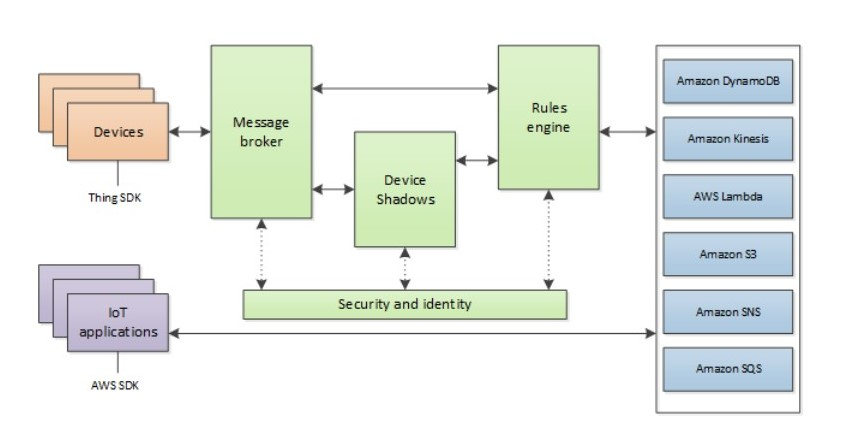
\includegraphics[width=0.9\columnwidth]{images/aws_structure}
	\end{center}
	\caption{Struttura della comunicazione}
	\label{fig:aws_structure}
\end{figure}


\subsubsection{Authentication}
AWS IoT Core offre autenticazione reciproca e crittografia in tutti i punti di connessione, perciò non si verificherà mai alcuno scambio di dati tra dispositivi e AWS IoT Core senza accertamenti di identità. AWS IoT Core supporta il metodo di autenticazione di AWS (denominato "SigV4"), l'autenticazione basata su certificato X.509 e l'autenticazione basata su token creati dal cliente (mediante autorizzazioni ad hoc). Le connessioni che impiegano il protocollo HTTP possono usare tutti i metodi disponibili, mentre le connessioni MQTT usano l'autenticazione basata su certificato e le connessioni WebSockets possono usare SigV4 o autorizzazioni ad hoc. È possibile mappare policy per ciascun certificato per autorizzare l'accesso di dispositivi e applicazioni e revocare l'accesso in qualsiasi momento senza toccare il dispositivo.

\begin{figure}
	\begin{center}
		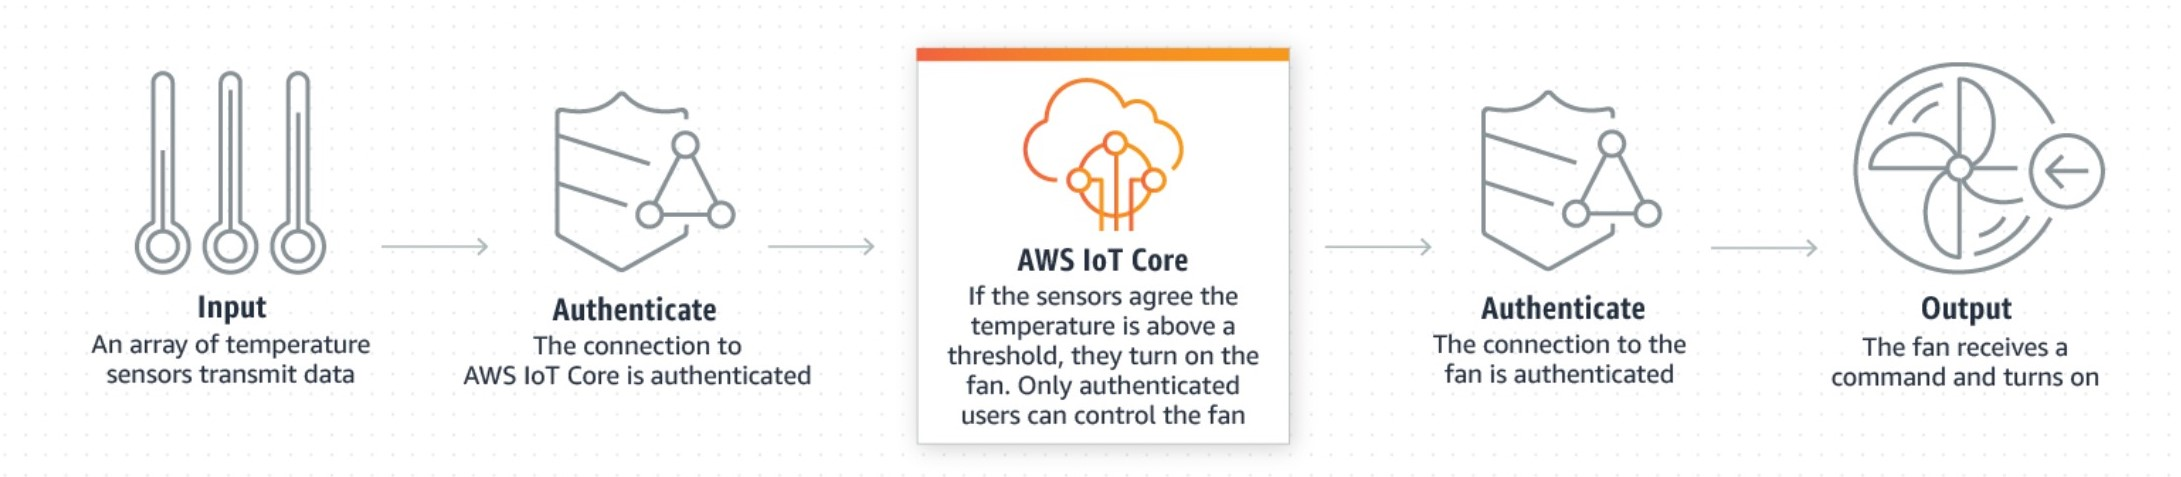
\includegraphics[width=0.9\columnwidth]{images/aws_auth}
	\end{center}
	\caption{Processo di autenticazione implementato in ogni punto della connessione}
	\label{fig:aws_auth}
\end{figure}

È possibile creare, distribuire e gestire certificati e policy per i dispositivi tramite la console o l'API. I certificati dei dispositivi possono essere assegnati, attivati e associati con le policy IoT corrispondenti configurate tramite AWS IoT Core. In questo modo sarà possibile revocare istantaneamente l'accesso per singoli dispositivi. AWS IoT Core supporta inoltre le connessioni dalle app per dispositivi mobili degli utenti tramite Amazon Cognito, che crea un identificatore univoco e recupera credenziali temporanee di AWS con privilegi limitati. AWS IoT Core fornisce inoltre credenziali AWS temporanee quando un dispositivo si autentica con un certificato X.509, per facilitare al dispositivo l'accesso ad altri servizi AWS, ad esempio DynamoDB o S3.

\subsubsection{Shadow dei Dispositivi}
Con AWS IoT Core è possibile creare versioni virtuali e persistenti dei dispositivi, chiamate "shadow" dei dispositivi (copia digitale del dispositivo), che includono l'ultimo stato noto del dispositivo, consentendo ad applicazioni e altri dispositivi di leggerne i messaggi e interagire con esso. La shadow dei dispositivi conserva l'ultimo stato noto e lo stato futuro impostato per ciascun dispositivo anche quando è offline. Per recuperare l'ultimo stato noto di un dispositivo o impostare uno stato futuro, è possibile usare l'API o il motore di regole.

La shadow dei dispositivi semplifica la creazione di applicazioni che interagiscono con i dispositivi perché fornisce sempre API REST disponibili. Inoltre, le applicazioni possono impostare uno stato futuro per un dispositivo indipendentemente dal suo stato corrente. AWS IoT Core confronterà lo stato futuro con l'ultimo stato noto e imporrà al dispositivo di aggiornarsi.

\subsection{AWS IoT Core Development}
\label{subsec:aws_dev}
Dopo aver visto le main features della cloud platform AWS IoT Core, si progettino ora gli step implementativi da seguire al fine di integrare correttamente il sistema progettato nelle precedenti sezioni con la cloud platform.
A tal scopo, sarà necessario seguire la documentazione messa a disposizione da AWS IoT Core per ottenere delle linee guida più dettagliate sui passi da seguire \url{https://docs.aws.amazon.com/it_it/iot/latest/developerguide/iot-dg.pdf}.\\
Gli step implementativi progettati in questa sezione si intendono riferiti ad una qualsiasi implementazione della cloud platform in un qualsiasi linguaggio di programmazione e per un qualsiasi progetto. I dettagli implementativi relativi al software sviluppato in questo lavoro di tesi, sarnno invece mostrati nel \autoref{chap:quattro}.\\
\begin{enumerate}
	\item Accesso alla Console AWS IoT Core e creazione di un nuovo account
	\item Registrazione e Configurazione di un nuovo dispositivo come copia digitale (o shadow) di un dispositivo reale
	\item Configurazione della comunicazione con il protocollo MQTT
	\item Utilizzo dell' SDK messa a sisposizione da AWS per l'abilitazione dei dispositivi IoT alla comunicazione con il Broker centrale.
\end{enumerate}

\subsubsection{Accesso alla Console AWS IoT Core}
Al fine di poter utilizzare i servizi offerti da AWS è necessario prima seguire un processo di registrazione di un nuovo account presso \url{https://aws.amazon.com/it/} e quindi seguire la procedura guidata per la Creazione di un Nuovo Account. \\
Una volta completata la procedura di resistrazione è quindi possibile accedere alla piattaforma IoT Core ed iniziare a creare un nuovo dispositivo.
\begin{figure}
	\begin{center}
		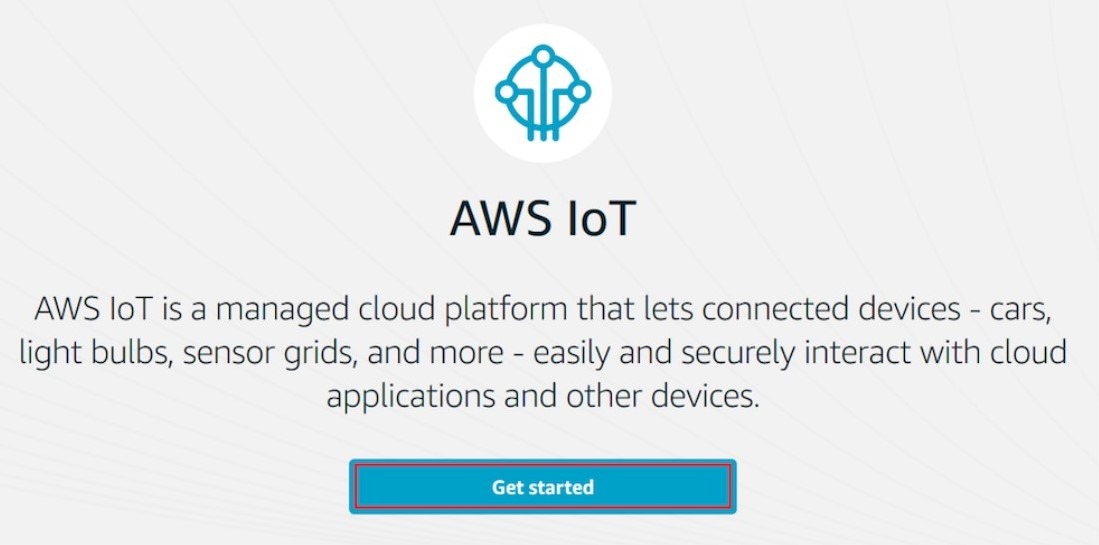
\includegraphics[width=0.9\columnwidth]{images/_1}
	\end{center}
	\caption{Primo accesso alla piattaforma IoT Core}
	\label{fig:_1}
\end{figure}

\subsubsection{Registrazione e Configurazione di un nuovo dispositivo}
I dispositivi connessi a AWS IoT sono rappresentati da oggetti IoT nel registro AWS IoT. Questo registro permette di tenere traccia di un record di tutti i dispositivi registrati nell'account AWS IoT in modo da poter assegnare a ciascun dispositivo diversi ruoli e quindi diverse permission.\\
Si rende quindi necessario creare ora una copia digitale di ogni dispositivo abilitato alla comunicazione con AWS IoT Core. In realtà, per evitare di creare un numero infinitamente grande di dispositivi diversi, un'approccio più adatto è quello di creare delle macro-categorie di oggetti che possono collegarsi alla piattaforma cloud. \\
Volendo, in questo lavoro di tes,i abilitare la comunicazione tra i soli smartphone con sistema operativo Android ed il Middleware IoT, si crei un unico oggetto denominato \textbf{Android\_Device} che si riferisca quindi a tutti i dispositivi Android che si collegano al Middleware. Allo stesso modo, è possibile creare una qualsiasi categoria di oggetti come ad esempio: \textbf{iOS\_Device}, \textbf{Windows\_Device}, \textbf{VMS\_Device}, etc.\\
La procedura per la creazione di un nuovo oggetto è descritta nei dettagli in \url{https://docs.aws.amazon.com/it_it/iot/latest/developerguide/iot-dg.pdf} ed il risultato finale sarà la comparsa di un nuovo prototipo di oggetto \textit{shadow} all'interno del IoT Core.
\begin{figure}
	\begin{center}
		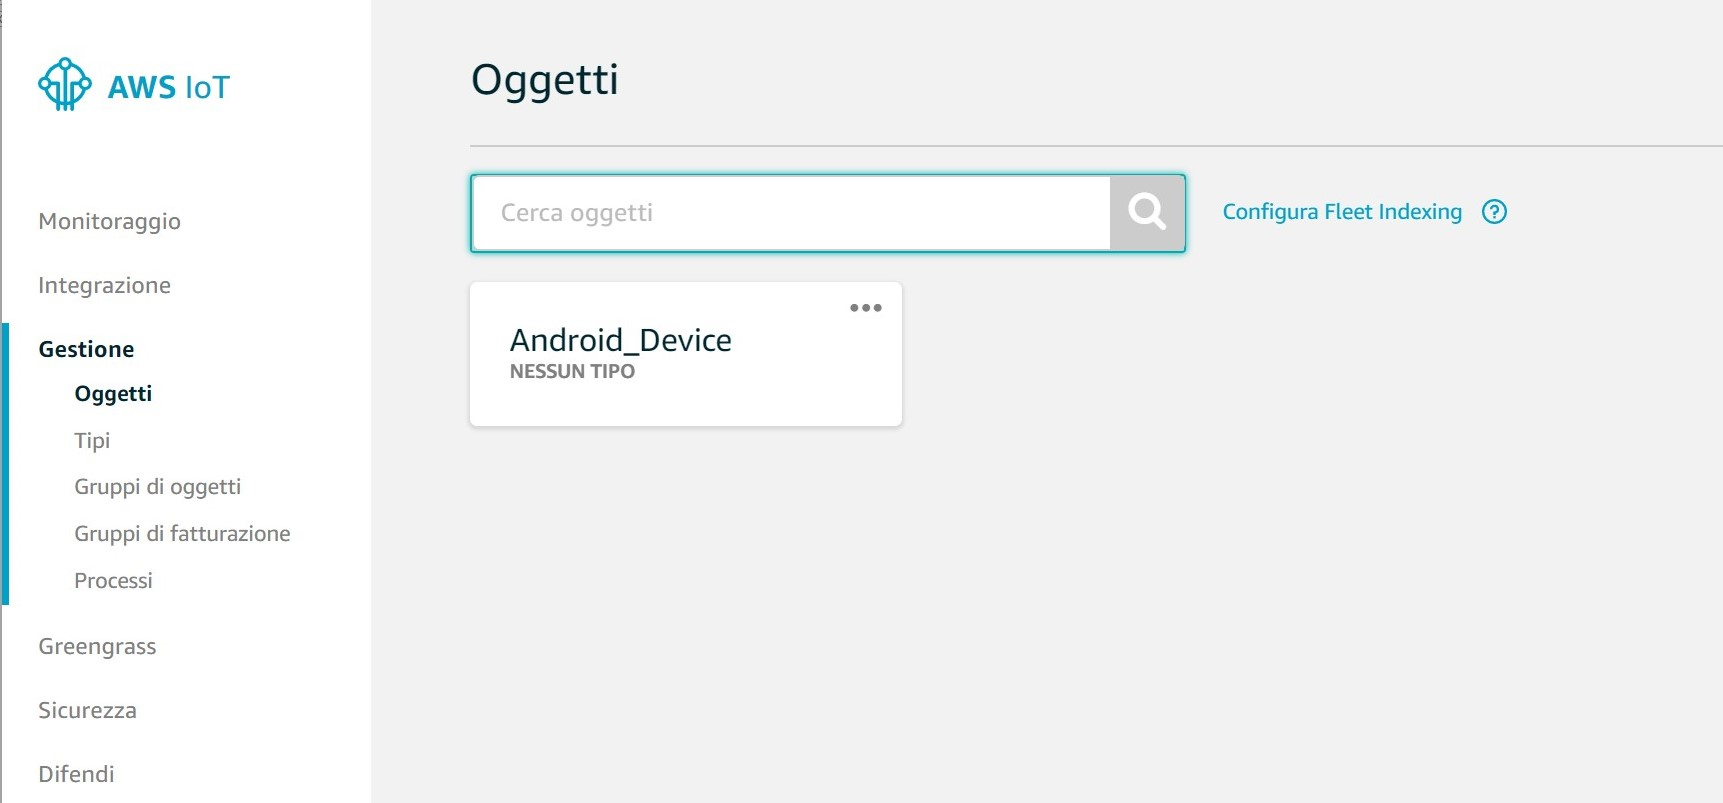
\includegraphics[width=0.9\columnwidth]{images/_2}
	\end{center}
	\caption{Creazione di un nuovo oggetto nella pagina principale di AWS IoT Core.}
	\label{fig:_2}
\end{figure}
Una volta creato, il nuovo dispositivo ha bisogno che vi siano assegnate delle perimission e quindi una Policy per poter comunicare con la Cloud Platform. AWS prevede infatti la possibilità di poter assegnare diverse Policy a diversi dispositivi che quindi avranno accesso a diverse componenti e servizi della Cloud Platform. Questo è fatto per garantire alti livelli di sicurezza e di gestione degli accessi a particolari servizi. Ad esempio, in questo modo potrebbero essere offerte alcune funzionalità a tutti i dispositivi, ed altre funzionalità premium ai soli dispositivi con un diverso piano tariffario.\\
Per lo scope di questo lavoro di tesi, la Policy che sarà assegnata al dispositivo appena creato (\textbf{Android\_Device}), sarà quella che gli consentirà di eseguire tutte le operazioni AWS IoT su tutte le risorse
AWS IoT. Queste impostazioni sono adatte ad un ambiente di sviluppo per facilitare il debugging ma sono ovviamente eccessivamente permissive ed è quindi opportuno restringere l'ambito delle autorizzazioni a quelle richieste dal dispositivo in un ambiente di produzione.\\
Anche in questo caso, per evitare ridondanze, si rimanda alla procedura per la creazione ed assegnazione di una nuova Policy ad un oggetto shadow creato, si rimanda alla documentazione ufficiale.

\subsubsection{Configurazione della Comunicazione}
\label{subsubsec:com}
A questo punto della configurazione, è possibile testare la comunicazione tra il Client (oggetto appena creato ed al quale è stata associata una Policy) ed il Server (IoT Core). \\
AWS IoT Core, consente inoltre di stabilire la comunicazione Client / Server seguendo diversi protocolli di comunicazione tra i quali MQTT ed HTTP che possono essere interscambiati a piacere.\\
In riferimento al \autoref{chap:introduzione} dove si era fatto un confronto tra i due protocolli e sui vantaggi dell'utilizzo di uno piuttosto che dell'altro, era evidente come il protocollo MQTT fossepiù efficiente in termini di consumo energetico e nella capacità comuputazionale richiesta. Pertanto, vista la frammentazione del mondo Android in termini di versioni del sistema operativo implementate ed anche in termini di obsolescenza dei dispositivi, si ritiene più adatto l'utilizzo del protocollo MQTT per stabilire una comunicazione tra il Client Android ed il server AWS.\\
\begin{figure}
	\begin{center}
		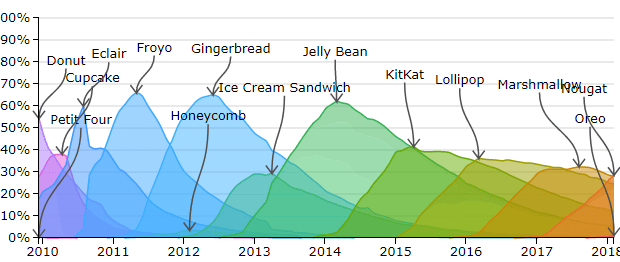
\includegraphics[width=0.9\columnwidth]{images/android_fragmentation}
	\end{center}
	\caption{Panorama della frammentazione nella distribuzione delle versioni del sistema operativo Android}
	\label{fig:android_fragmentation}
\end{figure}
Si testi quindi ora la comunicazione di tipo Publish - Subscribe tra il Client ed il Server (\autoref{sec:MQTT_protocol}).\\
Un dispositivo pubblicherà dei messaggi all'interno di un Topic ed è possibile impostare il Server IoT Core in modo da essere in ascolto sullo stesso Topic, caratterizzato cioè dallo stesso nome.\\
Nella sezione Test della console IoT Core, sono presenti due sottosezioni : \textbf{Pubblicare}  e \textbf{Sottoscrivere}.
\begin{figure}
	\begin{center}
		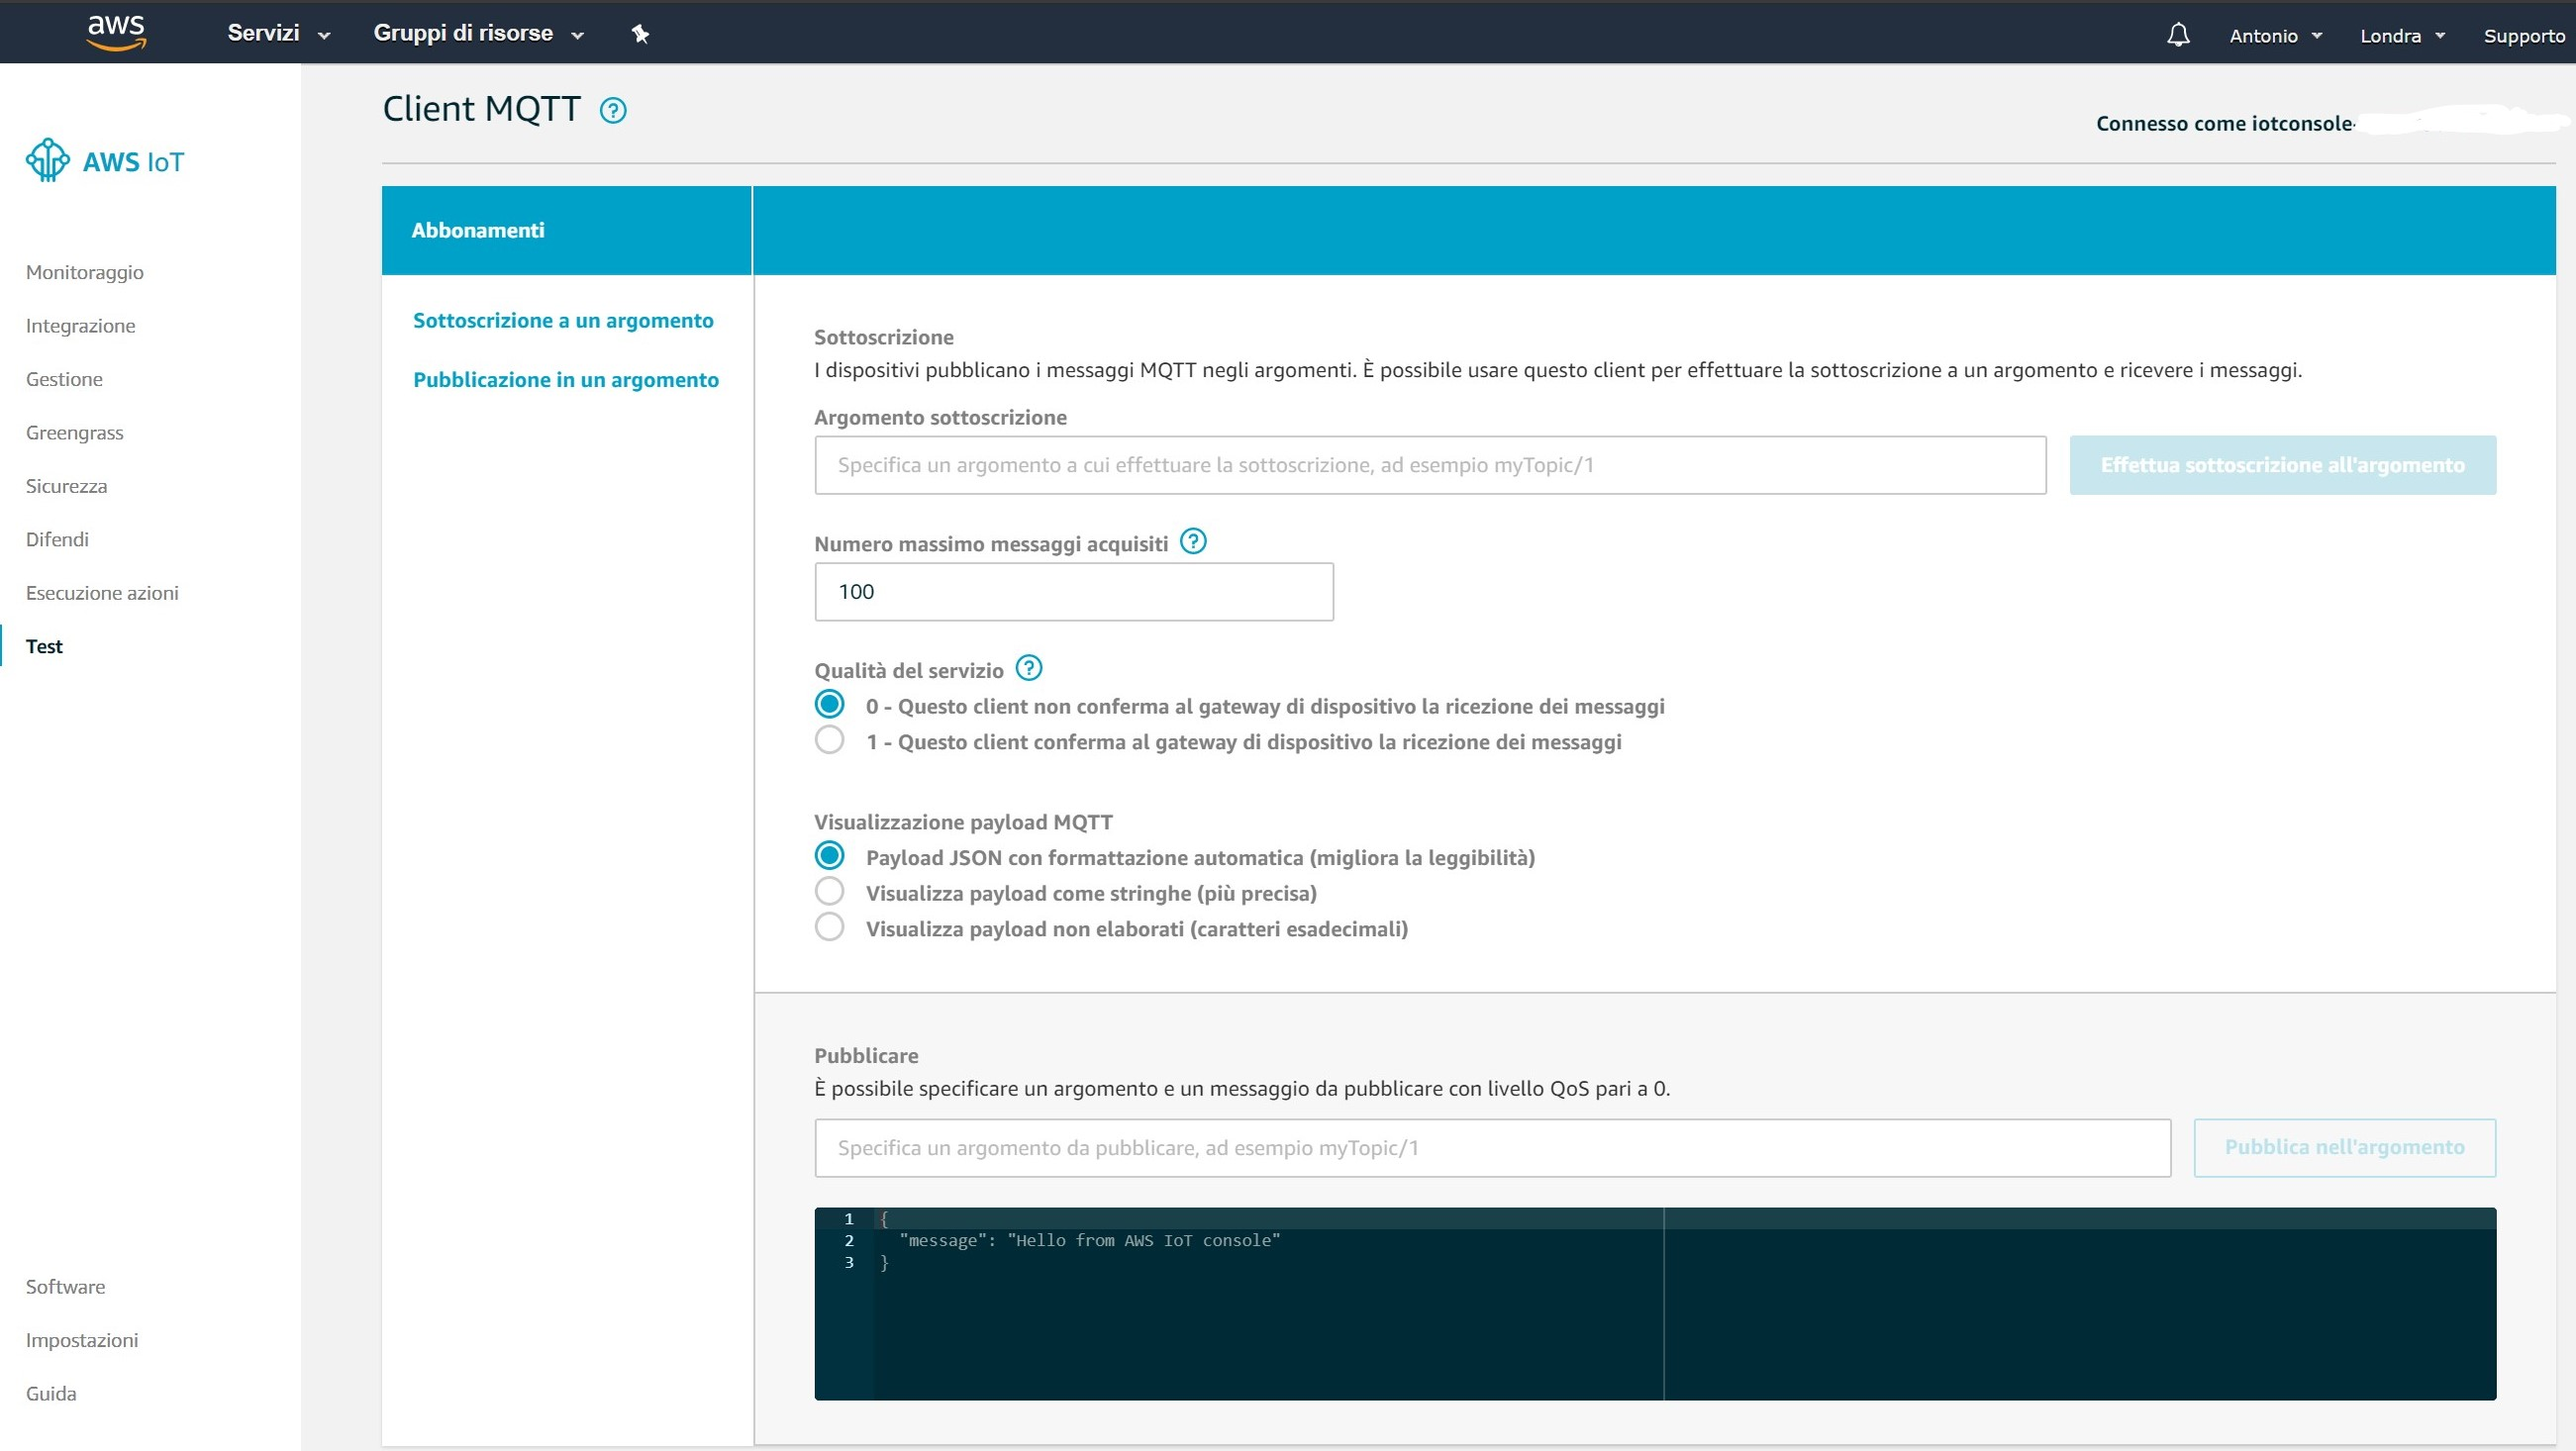
\includegraphics[width=1\columnwidth]{images/_3}
	\end{center}
	\caption{Panoramica della schermata Test}
	\label{fig:_3}
\end{figure}
Nella sezione \textbf{Sottoscrivere}, va specificato il nome del Topic al quale registrarsi o meglio sul quale restare in ascolto. Questo Topic sarà caratterizzato dsllo stesso nome del Topic sul quale il dispositivo comunicherà o meglio pubblicherà.
\begin{figure}
	\begin{center}
		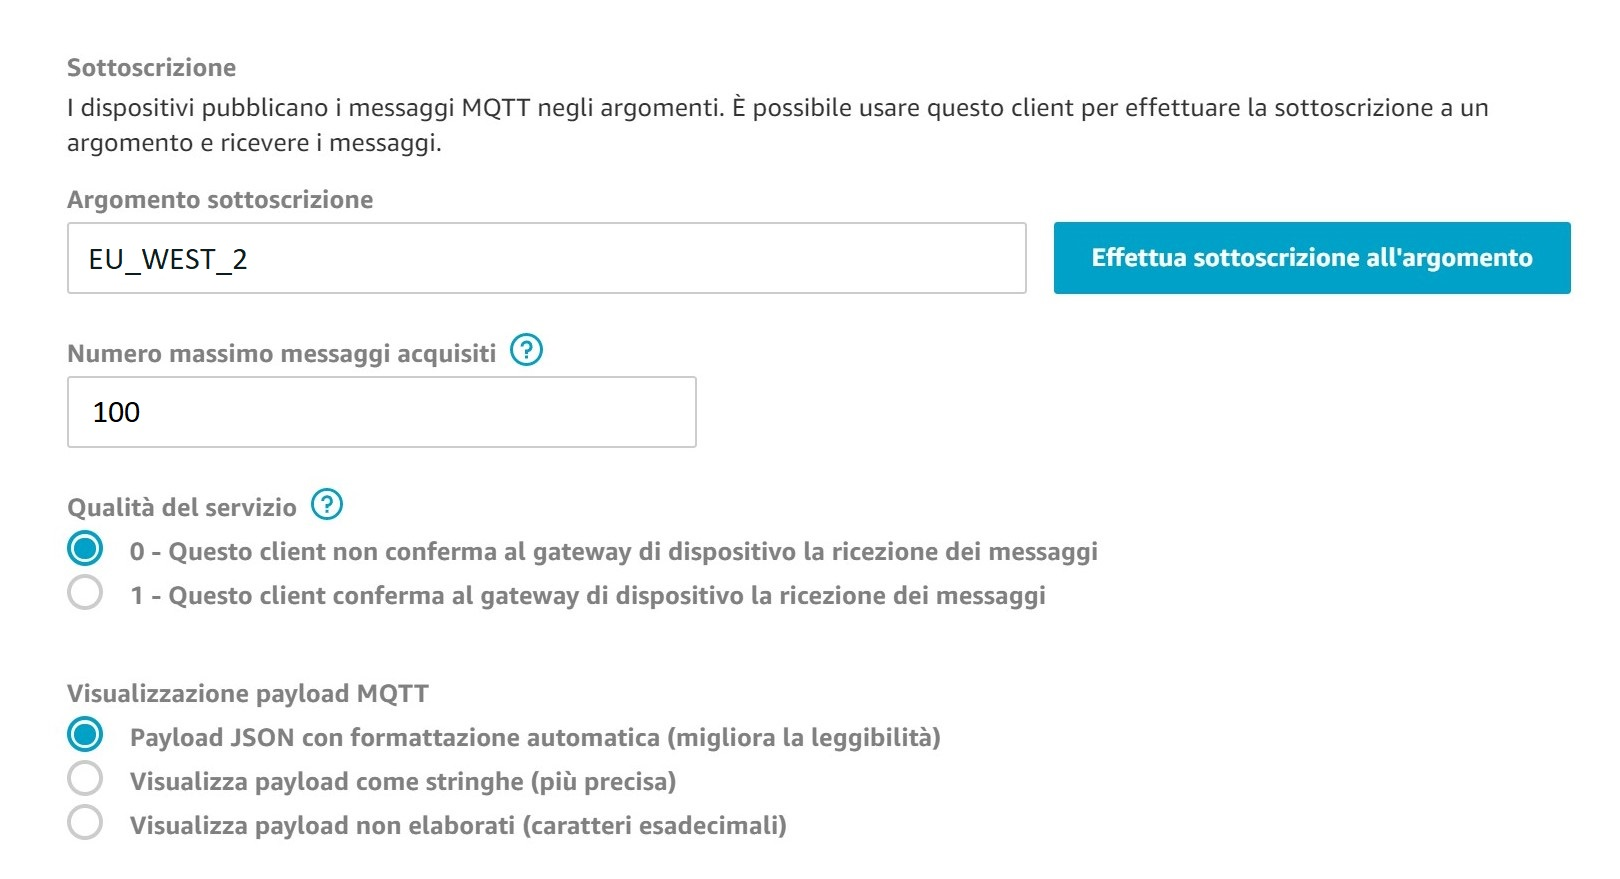
\includegraphics[width=0.8\columnwidth]{images/_4}
	\end{center}
	\caption{Sottoscrizione al Topic \textbf{EU\_WEST\_2}}
	\label{fig:_4}
\end{figure}
Infine, per simulare il comportamento di un dispositivo IoT che pubblichi un messaggio all'interno di un argomento, si pubblichi un messaggio nella sezione \textbf{Pubblicare} che faccia riferimento allo stesso topic sul quale si è in ascolto.
\begin{figure}
	\begin{center}
		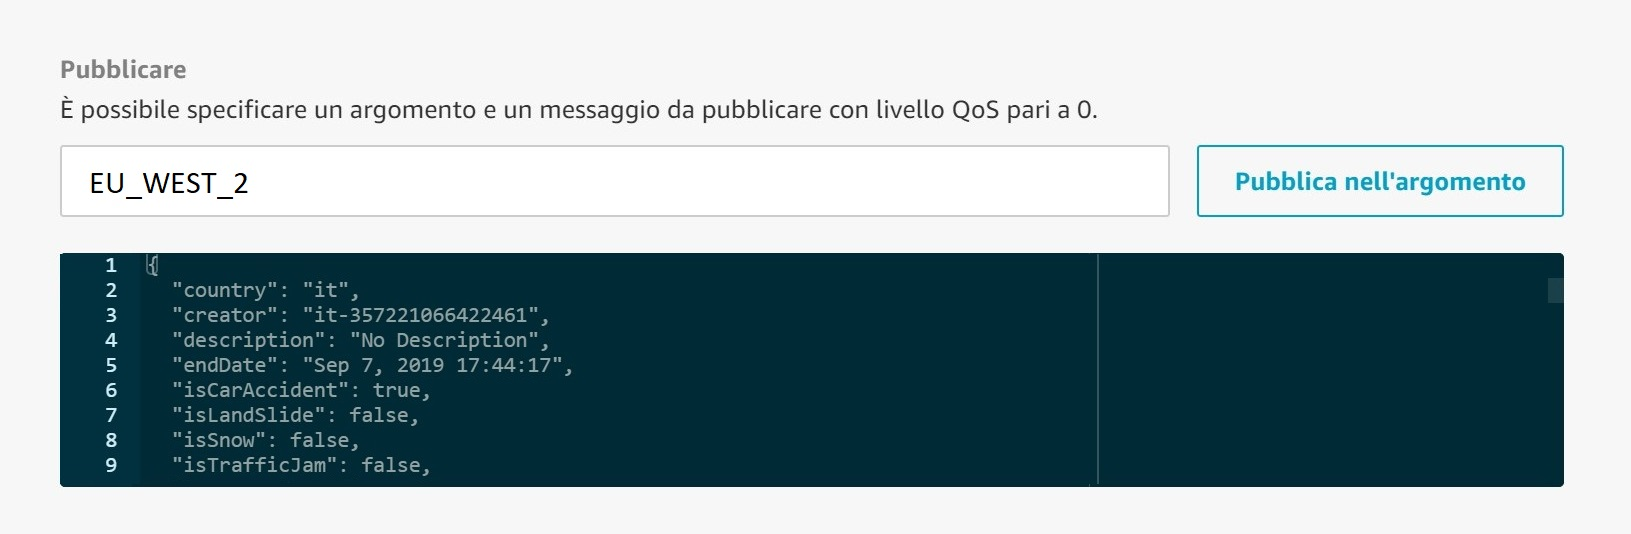
\includegraphics[width=1\columnwidth]{images/_5}
	\end{center}
	\caption{Pubblicazione nel Topic \textbf{EU\_WEST\_2}}
	\label{fig:_5}
\end{figure}
Dopo aver pubblicato il messaggio, nella sezione \textbf{Sottoscrivere} comparirà il messaggio appena ricevuto.
\begin{figure}
	\begin{center}
		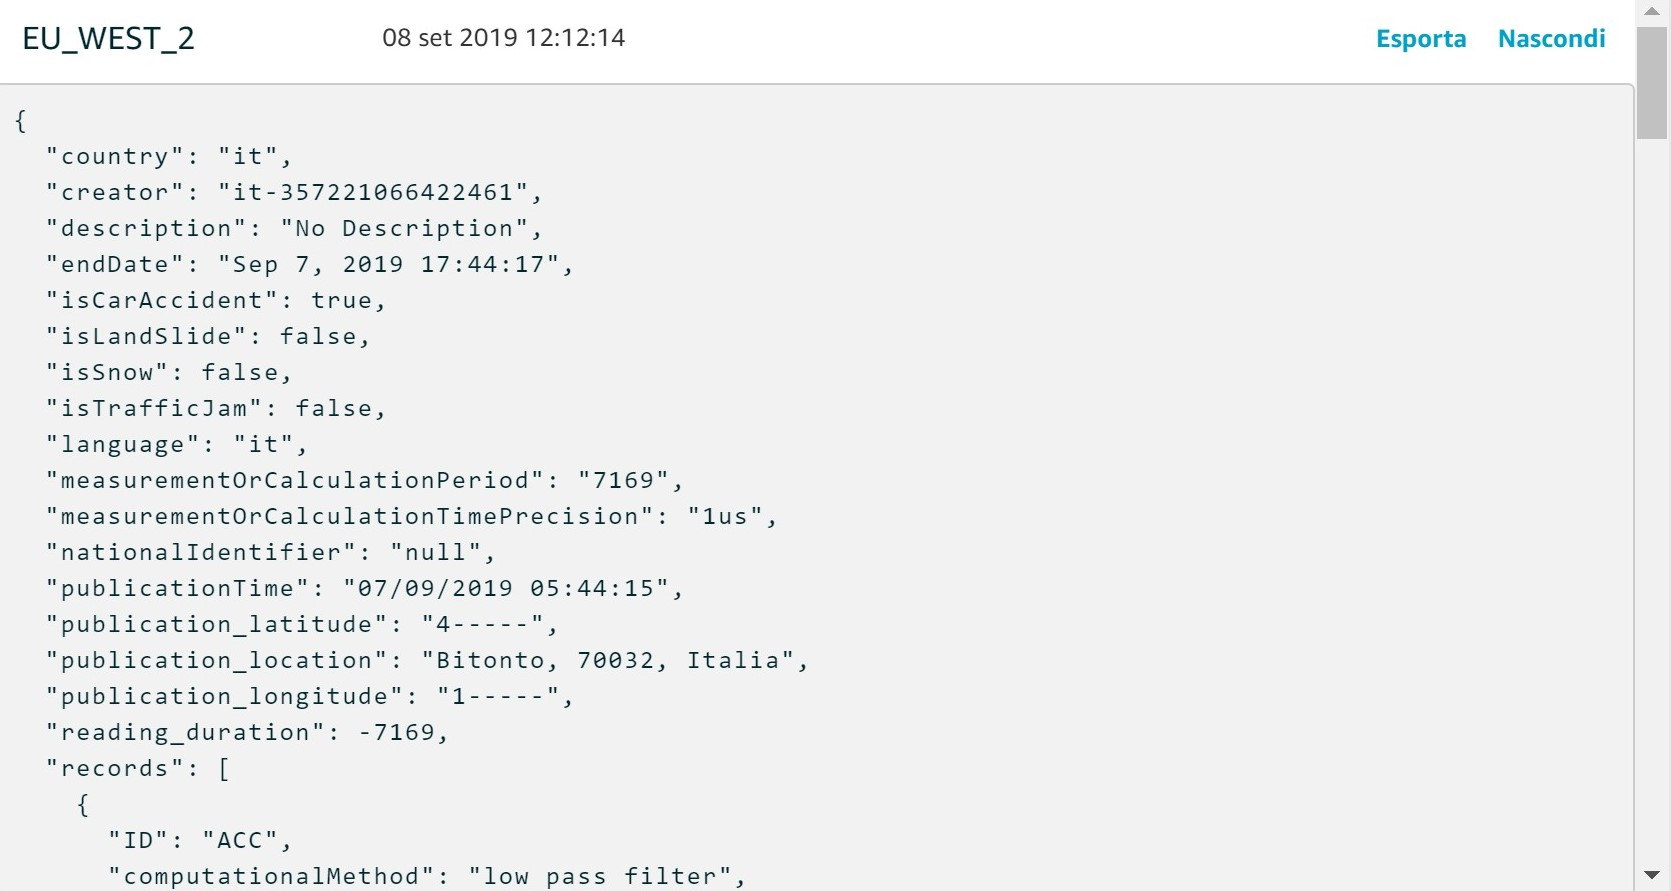
\includegraphics[width=1\columnwidth]{images/_6}
	\end{center}
	\caption{Ricezione del messaggio}
	\label{fig:_6}
\end{figure}
In maniera del tutto analoga, avverrà anche la comunicazione tra il Server IoT Core ed il Client Android. \\
Si noti come in \autoref{fig:_4}, \autoref{fig:_5} e \autoref{fig:_6} si è utilizzato come nome per il topic della pubblicazione \textbf{EU\_WEST\_2}. In realtà avremmo potuto ottenere lo stesso risultato e quindi stabilire la comunicazione tra client e server anche utilizzando un qualsiasi altro nome del topic, purchè il nome sul quale il Client pubblica i messaggi sia lo stesso sul quale il Server è in ascolto. Il motivo per cui sarà utilizzato il topic \textbf{EU\_WEST\_2} verrà spiegato nella \autoref{sec:aws_core}.

\subsubsection{Utilizzo della SDK}
Gli SDK (Software Development Kit) messi a disposizione dal team di sviluppo di AWS aiutano a connettere i dispositivi ad IoT Core in modo rapido e semplice.
Gli SDK di AWS IoT includono librerie open source, linee guida per gli
sviluppatori con esempi e guide alla portabilità, con cui è possibile creare soluzioni o prodotti IoT innovativi qualsiasi piattaforma hardware.\\
Gli SDK messi a disposizione dal team di AWS sono riferiti a specifiche architetture hardware e specifici linguaggi di programmazione e pertanto fuori dallo scope di questo capitolo che vuole invece fornire le linee guida generali di progettazione, indipendentemente dall'hardware e dal linguaggio utilizzato. Pertanto, nel \autoref{chap:quattro} saranno mostrati i dettagli implementativi dell' SDK per i dispositivi Android utilizzando il linguaggio di programmazione JAVA. \\
Qualora si vogliano ottenere i dettagli implementativi per altre piattaforme, si faccia riferimento alla documentazione ufficiale corredata anche da esempi applicativi (\url{https://docs.aws.amazon.com/it_it/iot/latest/developerguide/iot-dg.pdf}).
\begin{figure}
	\begin{center}
		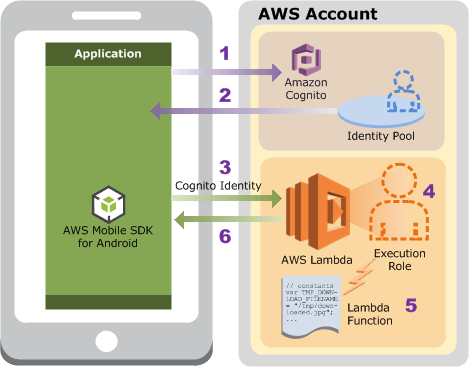
\includegraphics[width=0.5\columnwidth]{images/android_sdk}
	\end{center}
	\caption{Esempio dell'utilizzo dell'SDK messo a disposizione da AWS in Android per lo sviluppo di Lambda Application}
	\label{fig:android_sdk}
\end{figure}

\section{Database Architecture}
\label{sec:database}
In conclusione, l'utlima componente che è necessario progettare è il Database che si occuperà di raccogliere i dati provenienti da tutti i dispositivi IoT e transitanti attraverso la piattaforma cloud IoT Core. 
Il Database svolgerà un ruolo fodamentale in quanto non solo sarà il sistema di raccolta di tutti i dati provenienti da i dispositivi ma esso si occuperà anche di esporre questi stessi dati ad altre applicazioni che gli analizzeranno ed elaboreranno per trarne delle considerazioni e previsioni. Ulteriormente, i Database esporranno i dati in essi contenuti anche ad altri dispositivi IoT che dovessero interrogarli per ottenere informazioni sullo stato del traffico o in generale di eventi stradali.\\
Dal momento che la piattaforma Cloud che è stata scelta nella sezione precedente appartiene all'ecosistema AWS, è opportuno utilizzare un servizio di storage dei dati che appartenga allo stesso ecosistema in modo da sfruttare l'ampia documentazione e la facilità di interfacciamento dei due sistemi appartenenti allo stesso ecosistema. In tal caso, AWS mette a disposizione due servizi per lo storage dei dati:
\begin{itemize}
	\item \textbf{Amazon RDS: } Servizio per l'utilizzo di Database Relazionali (SQL)
	\item \textbf{Amazon DynamoDB: } Servizio per l'utilizzo di Database Non Relazionali (NoSQL)
\end{itemize}
La differenza sostanziale tra i due servizi consiste quindi nella architettura di Database nella quale si vogliono raccogliere i dati.\\
Si evidenzino quindi i requisiti che il Database deve soddisfare per il Software che si sta progettando in modo da vedere quali delle due servizi offerti da AWS sia più consono al progetto.\\
\begin{longtable}{|m{2cm}|m{12cm}|}
	\hline
	\textbf{Requisito} & \textbf{Descizione} \\
	\hline
	\textbf{D1} &   Il Database dovrà essere altamente scalabile per sopperire ad un numero di dispositivi e di entry nel database molto elevato \\
	\hline
	\textbf{D2} &   Il Database dovrà essere altamente performante per rispondere  in breve tempo alle query \\
	\hline
	\textbf{D3} &   Il Database dovrà supportare l'invio di query geo-referenziate \\
	\hline
	\textbf{D4} &   Il Database dovrà supportare e memorizzare diverse tipologie di dati provenienti da diversi dispositivi \\
	\hline
	\textbf{D5} &   Il Database dovrà essere progettato considerando il suo futuro utilizzo per la Big Data Analysis  \\
	\hline
	\caption{Analisi dei requisiti che la IoT Cloud Platform deve supportare}
	\label{tabel:requisiti_database}
\end{longtable}
Per capire quindi quale soluzione meglio si adatta ai requisiti del progetto in fase di sviluppo, è necessario effettuare una breve digressione sulle differenze tra le due architetture di un Database in modo da averne chiari i punti di forza ed i punti deboli di ciascuna architettura.\\

\subsection{Database Relazionali e Non Relazionali}
I Database Relazionali o \textbf{RDBMS} memorizzano i dati in tuple o record ovvero salvano i dati all'interno di tabelle. Ciascuna tabella ha un numero fisso di colonne e un numero variabile di righe (o record). Le colonne definiscono i dati degli attributi elle entità di una data tabella. Ad esempio, una tabella clienti avrà come colonne nome, cognome, indirizzo, telefono, e così via. Ogni riga nella tabella definisce un elemento effettivo costituito da valori per tutte le colonne.\\
Le tabelle hanno colonne speciali chiamate chiavi primarie (primary key), che contengono identificatori unici per ogni riga di una tabella. Le tabelle possono anche avere delle colonne chiamate chiavi esterne (foreign key), che contengono un riferimento chiave primaria di una riga su un’altra tabella (o anche sè stessa). Questi collegamenti tra righe sono chiamate associazioni (o relazioni, dall’inglese relationships) e sono la base del modello relazionale di un database.\\
\begin{figure}
	\begin{center}
		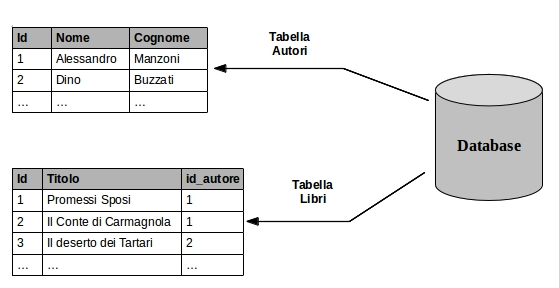
\includegraphics[width=0.5\columnwidth]{images/relational_db}
	\end{center}
	\caption{Esempio di un database relazionale}
	\label{fig:relational_db}
\end{figure}
I database relazionali trovano spazio d’applicazione quando si ha a che fare con dati strutturati, ovvero quando è facile creare una rappresentazione su tabella semplice e lineare, con un numero ridotto di relazioni. Inoltre, gli SQL sono praticamente obbligatori ogni volta che dobbiamo garantire integrità sui dati e le proprietà ACID in senso lato.\\
I Database Non Relazionali o \textbf{NRDBMS} utilizzano molteplici modelli di dati per accedere e gestire i dati, quali documento, grafo, chiave-valore, in memoria e ricerca. Questi tipi di database sono ottimizzati specificatamente per applicazioni che necessitano di grandi volumi di dati, latenza bassa e modelli di dati flessibili, ottenuti snellendo alcuni dei criteri di coerenza dei dati degli altri database. I database NoSQL sono una soluzione ideale per molte applicazioni moderne, quali dispositivi mobili, Web e videogiochi che richiedono database flessibili, scalabili, con prestazioni elevate ed altamente funzionali per offrire un'esperienza utente eccezionale.\\
I NoSQL sono estremamente versatili e quindi indicati in quelle situazioni in cui dobbiamo modellare il polimorfismo. Se si hanno entità tra loro tutte simili e che grossomodo portano la stessa informazione, ma con piccole differenze l’una dall’altra, con NoSQL il problema si risolve qualche manciata di minuti. In SQL, invece, è necessaria una soluzione decisamente più complessa. NoSQL è quindi ideale nel caso di dati abbastanza scorrelati e che tendono ad evolvere nel tempo; l’assenza di una struttura fissa permette di aggiungere nuovi tipi di dati (o modificare gli esistenti) senza dover mettere mano al database.
\begin{figure}
	\begin{center}
		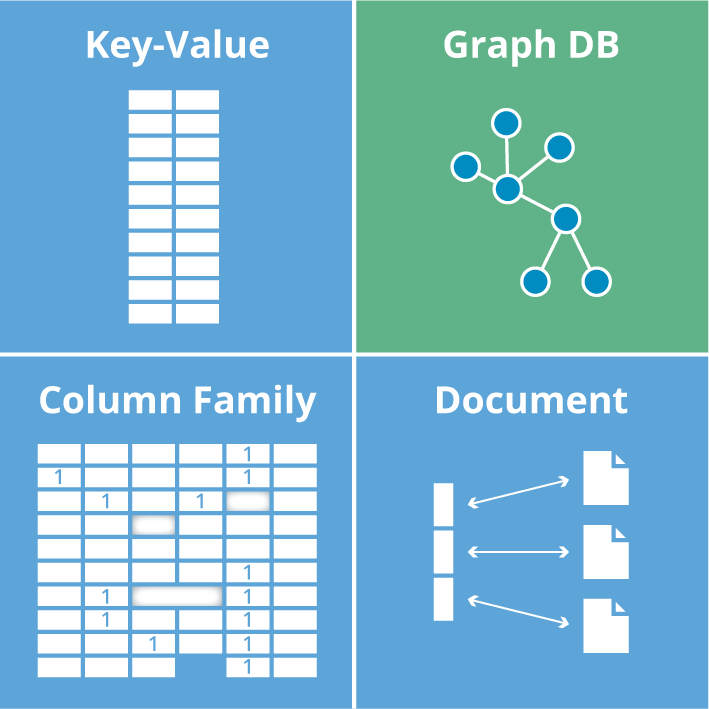
\includegraphics[width=0.45\columnwidth]{images/nonrelational_db}
	\end{center}
	\caption{Esempio di un database non relazionale}
	\label{fig:nonrelational_db}
\end{figure}

\subsection{Query Geo-Referenziate}
Una delle prerogative principali che il Database deve supportare sono la possibilità di rispondere a query geo-referenziate. Questo significa che un utente debba essere in grado di interrogare il Database per ricevere i soli eventi avvenuti in una certa area geografica. Allo stesso modo, anche la analisi dei dati può essere effettuata in forma locale in modo da poter eventualmente fornire diverse previsioni e considerazioni per diverse aree geografiche in funzione delle prerogative di quella particolare area. Questo implica delle scelte progettuali che tengano conto di questa prerogativa in modo da ottimizzare questo aspetto nella costruzione dell'architettura del Database.\\
Notevoli sono gli sforzi della ricerca per lo studio delle migliori architetture di Database che garantissero ottime performance quando sottoposti a query geo-referenziate. Nei lavori \cite{famous:paper_detti_1} e \cite{famous:paper_detti_2} viene progettato uno Spatial Database di tipo ICN (Information Centric Networking) denominato OpenGeoBase. Attraverso l'architettura implementata, il Database può facilmente lavorare in maniera distribuita, usando anche differenti Database Engines in parallelo. In questo modo, si realizza una architetture multi-tenant nella quale diversi utenti e diversi processi possono concorrere indipendentemente all'uso del Database. Ulteriormente, in \cite{famous:paper_detti_1} e \cite{famous:paper_detti_3} si dimostra come una implementazione di una simile architettura di Database sia particolarmente adatta ad applicazioni di ITS (Intelligent Transportation System) in quanto consenta l'esecuzione di query geo-referenziate. OpenGeoBase memorizza i dati geo-referenziati in formato GeoJSON supportando così query riferite ad una certa area geografica. Nella fattispecie, le funzionalità implementate da OpenGeoBase sono:
\begin{itemize}
	\item Routing-by-name per l'invio di query e l'inserimento di nuovi dati
	\item In-Networking caching per velocizzare le query e ridurre i tempi di calcolo del Database Engine
	\item Sicurezza di tipo Data-Centric per il supporto di applicazioni multi-tenant
\end{itemize}
Gli Spatial Database sono solitamente implementati come estensioni o plug-in di DBMS (Database Management System) generici. Tuttavia, in quanto Database Relazionali di tipo SQL, queste soluzioni sono affette da problemi di performamnces nel momento in cui le simensioni del Database aumentano. Pertanto, per grandi raccolte di dati (Big Data), i Database NoSQL stanno sempre più prendendo piede rimpiazzando i Database Relazionali in quanto i Non Relazionali risultano più semplici da distribuire in diversi Server. Sebbene un DBMS Relazionale possa offrire un numero maggiore di strumenti per la gestione e creazione di query, in applicazioni dove sono richieste soltanto delle semplici operazioni di read/write su grosse moli di dati, i Database NoSQL sono ritenuti più adatti in quanto possono essere più facilmente distribuiti.
\begin{figure}
	\begin{center}
		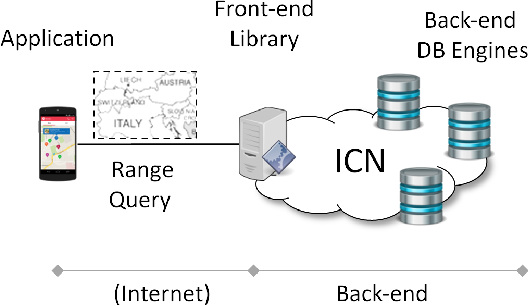
\includegraphics[width=0.6\columnwidth]{images/opengeobase_1}
	\end{center}
	\caption{Architettura di OpenGeoBase \cite{famous:paper_detti_1}}
	\label{fig:opengeobase_1}
\end{figure}
\begin{figure}
	\begin{center}
		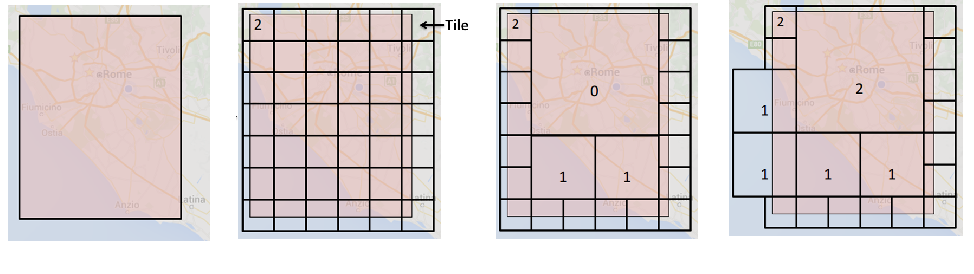
\includegraphics[width=0.8\columnwidth]{images/opengeobase_2}
	\end{center}
	\caption{Range-Query ed approcci di suddivisione della griglia basata su tre livelli 0,1,2 \cite{famous:paper_detti_1}}
	\label{fig:opengeobase_2}
\end{figure}


Alla luce di quanto detto, è subito evidente che una simile architettura di Database proposta in \cite
{famous:paper_detti_1} e \cite{famous:paper_detti_2} bene si adatti ai requisiti del sistema in fase di progettazione illustrati nella \autoref{tabel:requisiti_database}. Pertanto, alla luce del confronto tra Database Relazionali e Non, ed al fine di rendere il sistema in fase di sviluppo compatibile con l'implementazione di uno Spatial Database come OpenGeoBase, la scelta è ricaduta sull'utilizzo di un Database Non Relazionale e quindi NoSQL. Pertanto, dall'ecosistema AWS si è scelto di utilizzare Amazon DynamoDB.

\subsection{Amazon DynamoDB}
\label{subsec:dynamodb}
Amazon DynamoDB è il servizio di memorizzazione dei dati in Database Non Relazionali di tipo NoSQL. DynamoDB supporta i modelli di dati di tipo documento e di tipo chiave-valore ed è quindi adatto alla memorizzazione dei dati in formato JSON.\\
DynamoDB supporta due tipi di chiavi primarie:
\begin{itemize}
	\item \textbf{Partition key: } Una semplice chiave primaria, composta da un attributo chiamato \textit{partition key}. Gli attributi in DynamoDB sono simili in molti modi ai campi o alle colonne di altre arcitetture di Database
	\item \textbf{Partition key and Sort key: } Si riferiscono ad una chiave primaria composta da due attributi. Il primo attributo è la partition key ed il secondo attributo è chiamato \textit{sort key}
\end{itemize}
\begin{figure}
	\begin{center}
		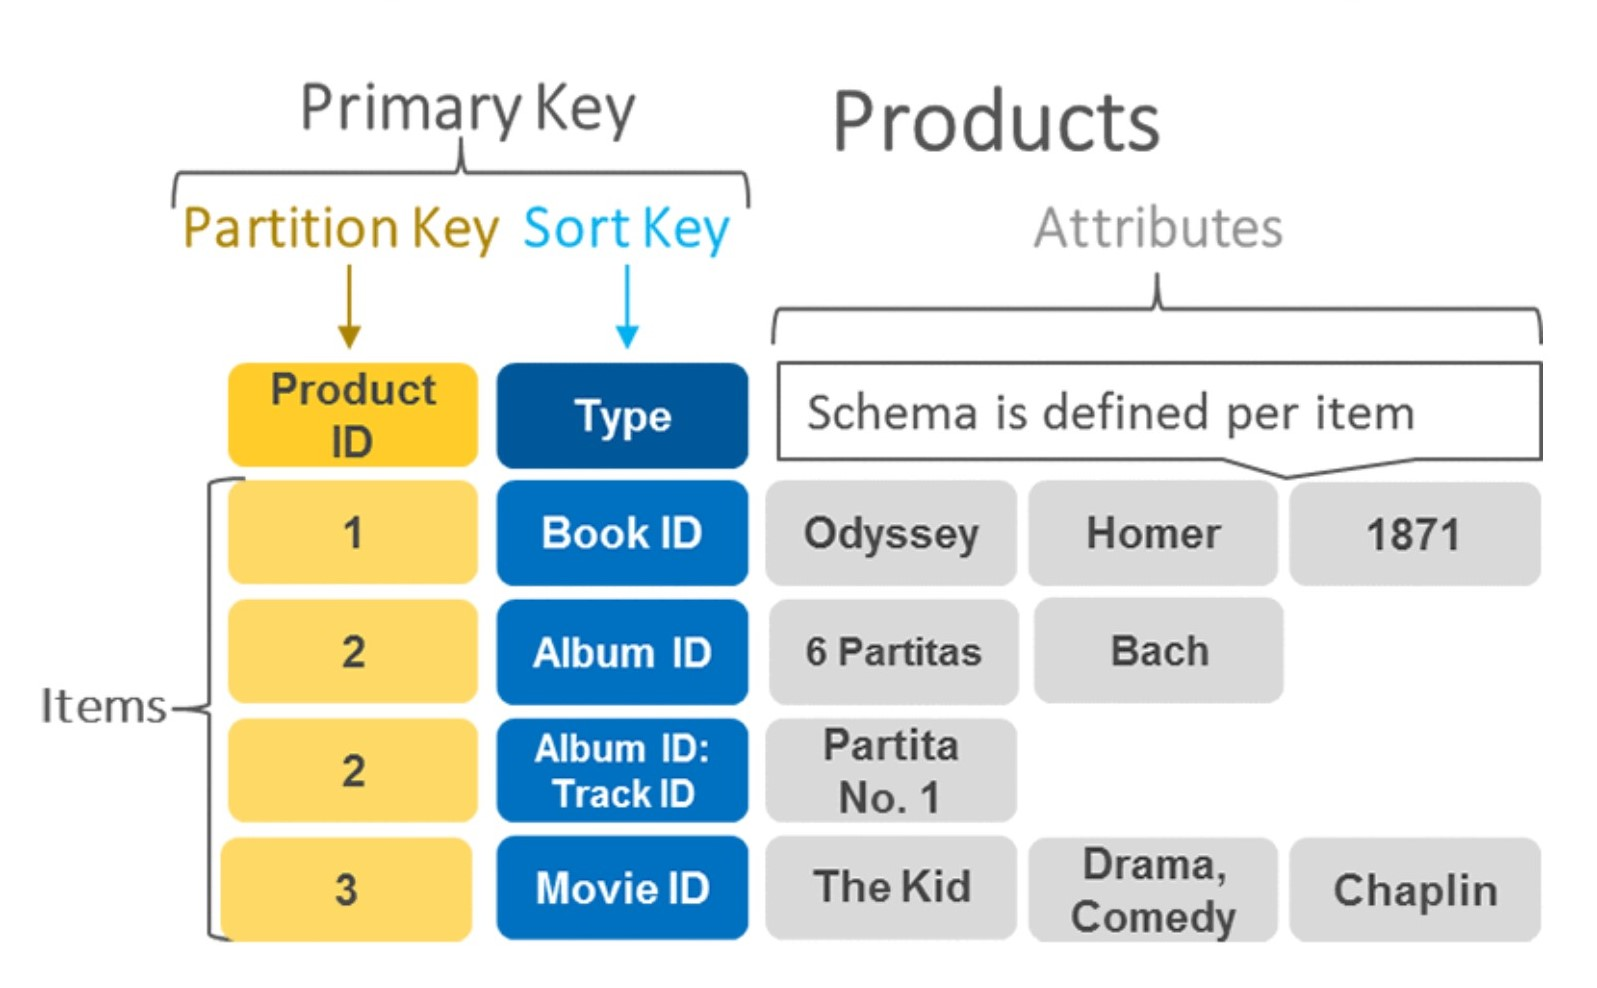
\includegraphics[width=0.7\columnwidth]{images/dynamodb_1}
	\end{center}
	\caption{Schema di una tabella in DynamoDB evidenziando i campi \textit{partition key} e \textit{sort key}}
	\label{fig:dynamodb_1}
\end{figure}
DynamoDB memorizza i dati come gruppi di attributi, chiamati \textit{items}. Gli \textit{items} sono simili alle righe o tuple o record in altri Database. Ciascun \textit{item} viene memorizzato e recuperato utilizzando la sua chiave primaria che deve quindi essere unica. Gli \textit{item} sono inoltre memorizzati in unità da 10GB chiamate partitions come mostrato in \autoref{fig:dynamodb_2}. Pertanto, tutti gli \textit{item} aventi lo stesso partition key sono memorizzati insieme, cioè nella stessa partition e sono ordinati in funzione del valore della loro sort key.
\begin{figure}
	\begin{center}
		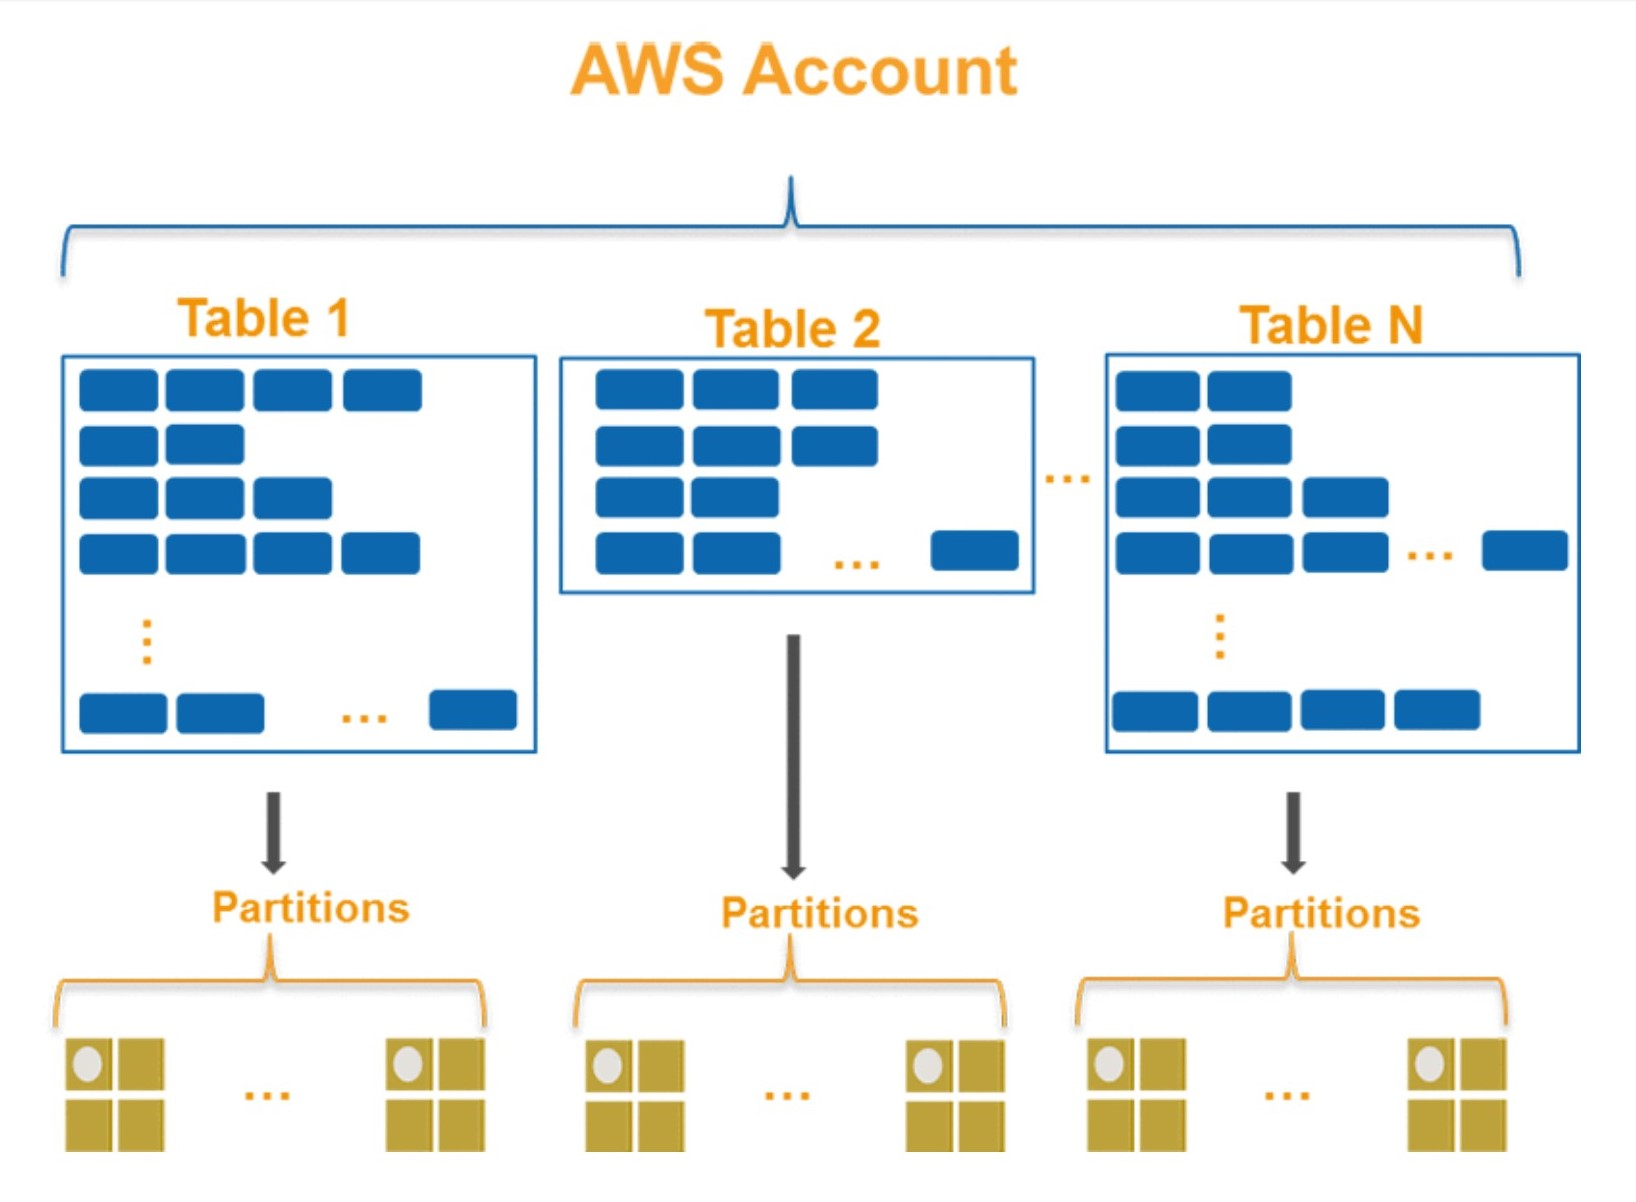
\includegraphics[width=0.6\columnwidth]{images/dynamodb_2}
	\end{center}
	\caption{Suddivisione di un Database in DynamoDB in tabelle e suddivisione delle tabelle in Partitions}
	\label{fig:dynamodb_2}
\end{figure}

A seguito della overview mostrata su DynamoDB, si ha ora a disposizione uno schema implementativo di un Database con DynamoDB. Pertanto, ora si può procedere al collegamento tra la Cloud Platform IoT Core progettata in precedenza ed il Database DynamoDB. Questa comunicazione sarà necessaria per fare in modo che i dati ricevuti dalla Cloud Platform IoT Core siano automaticamente memorizzati all'interno delle tabelle del Database che saranno poi utilizzate per le query degli uteni e per l'analisi dei dati. Una volta stabilita la comunicazione tra IoT Core e DynamoDB, nel \autoref{chap:quattro} sarà mostrata una implementazione di questa comunicazione e come sia possibile interrogare DynamoDB da uno smartphone android per visualizzarne i dati.\\
Per stabilire il collegamento tra IoT Core e DynamoDB è necessario creare una \textbf{regola} in DynamoDB che consenta di recuperare informazioni da un messaggio MQTT in ingresso e di scriverle in una tabella DynamoDB. I passi da seguire sono quindi:
\begin{itemize}
	\item Creazione di una nuova regola in AWS IoT Core
	\item Creazione di una nuova tabella in DynamoDB
	\item Creazione di un nuovo ruolo
	\item Test della comunicazione
\end{itemize}
Per avere un maggiore livello di dettaglio sull'implementazione di ciascuna fase, si faccia riferimento alla documentazione ufficiale \url{https://docs.aws.amazon.com/it_it/iot/latest/developerguide/iot-dg.pdf}.

\subsubsection{Creazione di una nuova Regola}
Con la creazione di una nuova Regola si vuole automatizzare il processo di comunicazione tra la piattaforma IoT Core ed il Database DynamoDB. In questo modo, ogni qual volta IoT Core riceve una nuova entry da dispositivi IoT, dopo aver eventualmente verificato e validato i dati, può memorizzarli in un Database per future elaborazioni ed analisi. \\
Per creare una nuova regola, si acceda alla piattaforma AWS IoT Core come spiegato nella \autoref{sec:iot_core} e nel riquadro di navigazione cliccare su \textit{Agisci} e quindi nella pagina \textit{Regole} cliccare su \textit{Crea una Regola}.A questo punto, nella pagina di creazione della nuova regola dovremmo inserire le caratteristiche della regola come Nome e Descrizione. Il campo \textit{Istruzione query della Regola} scegliere la versione più recente del campo Uso di SQL. Infine, nel campo \textit{Istruzioni query della Regola} va immessa la query in linguaggio SQL da eseguire quando viene attivata la regola.\\
\begin{figure}
	\begin{center}
		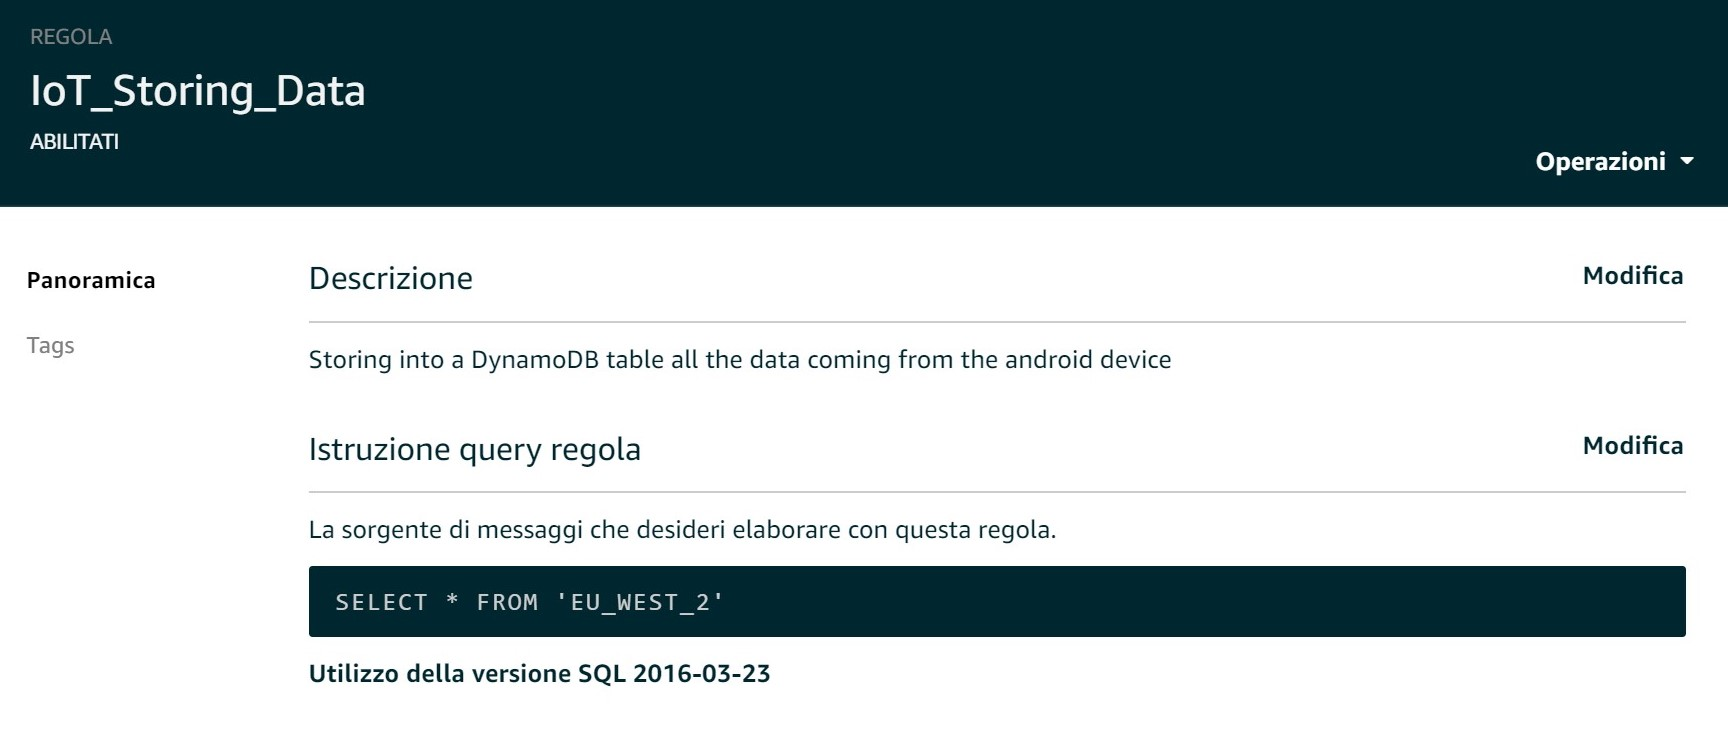
\includegraphics[width=0.7\columnwidth]{images/dynamodb_3}
	\end{center}
	\caption{Visualizzazione della Regola sul database DynamoDB}
	\label{fig:dynamodb_3}
\end{figure}
In questo caso, l'istruzione SQL che sarà eseguita consiste in una interrogazione di tutti i dati contenuti in una tabella di DynamoDB.

\subsubsection{Creazione di una nuova Tabella}
Una volta creata la regola in IoT Core, va ora creata e collegata ad una tabella di DynamoDB. Pertanto, nella pagina \textit{Seleziona un'operazione}, scegliere \textit{Inserisci un messaggio in una tabella DynamoDB} e quindi su \textit{Configura Operazione}.
\begin{figure}
	\begin{center}
		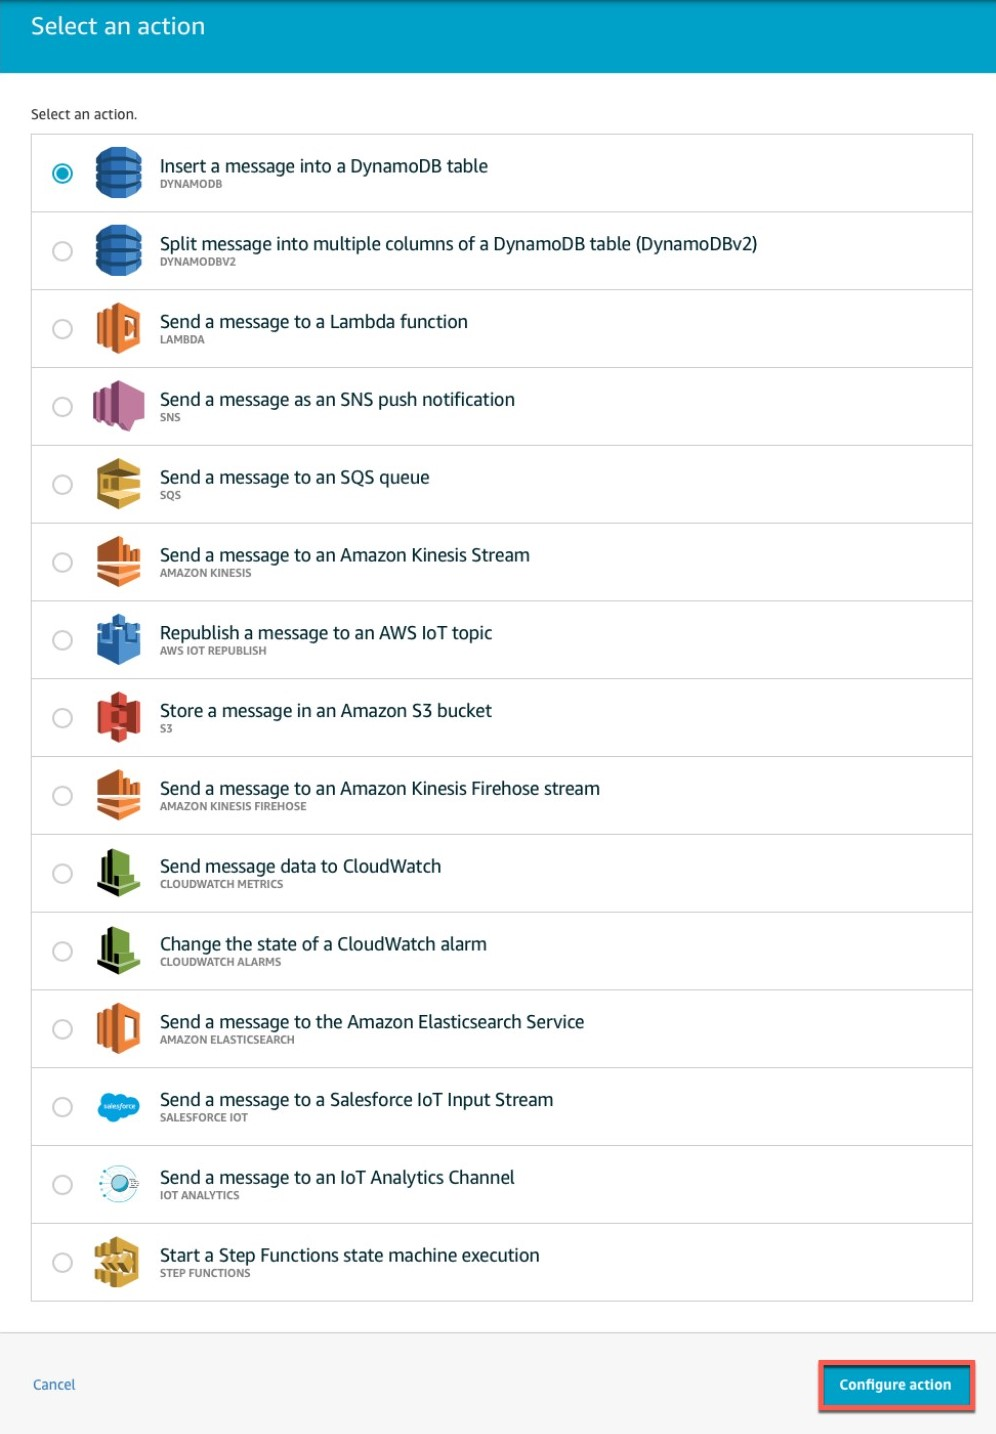
\includegraphics[width=0.58\columnwidth]{images/dynamodb_4}
	\end{center}
	\caption{Creazione di una nuova tabella}
	\label{fig:dynamodb_4}
\end{figure}
Nella pagina \textit{Configura Operazione} scegliere \textit{Crea una nuova Risorsa} e quindi nella pagina di DynamoDB scegliere \textit{Crea Tabella}.Nella pagina \textit{Crea tabella DynamoDB}, compilare i campi relativi alle informazioni della nuova tabella come Nome, Chiave di Partizione e Chiave di Ordinamento. Questi nomi, per testare un primo esempio di comunicazione, sono stati impostati a Row e PoistionInRow. Questi nomi assegnati alle colonne della tabella di DynamoDB dovranno rispettare quelli che saranno ricevuti all'interno del messaggio JSON ricevuto da DynamoDB.\\
Nel campo \textit{Partizione} e \textit{Chiave di ordinamento} scegliere String e quindi creare la nuova tabella con un click sul pulsante \textit{Crea}.\\
A questo punto, la tabella di DynamoDB è creata e si può chiudere la scheda del browser in cui è aperta la console Amazon DynamoDB.
A questo punto, nella console di AWS IoT Core precedentemente in fase di configurazione sarà visibile, nell'elenco delle tabelle, la tabella appena creata.


\subsubsection{Creazione di un nuovo Ruolo}
Una volta creata la nuova tabella in DynamoDB, è ora necessario fornire l'accesso alla lettura e scrittura di questa tabella ad IoT Core. Pertanto, nella console IoT Core, nella sezione \textit{Configura Operazione}, selezionare la tabella appena creata dall'elenco.\\
Quindi bisogna configurare i dettagli della comunicazione tra IoT Core e DynamoDB e, nel campo \textit{Partition Key} immettere \${row}. In questo modo, si indica alla regola di recuperare il valore dell'attributo row dal messaggio MQTT e di scriverlo nella colonna row della tabella DynamoDB. In \textit{Sort Key}, immettere \${pos}. In questo modo, il valore dell'attributo pos viene scritto nella colonna PositionInRow. Per impostazione predefinita, l'intero messaggio viene scritto in una
colonna della tabella denominata Payload. \\
Scegliere quindi \textit{Crea un nuovo ruolo} per procedere alla creazione di un nuovo ruolo da associare ad IoT Core per l'accesso alla tabella di DynamoDB. 
\begin{figure}
	\begin{center}
		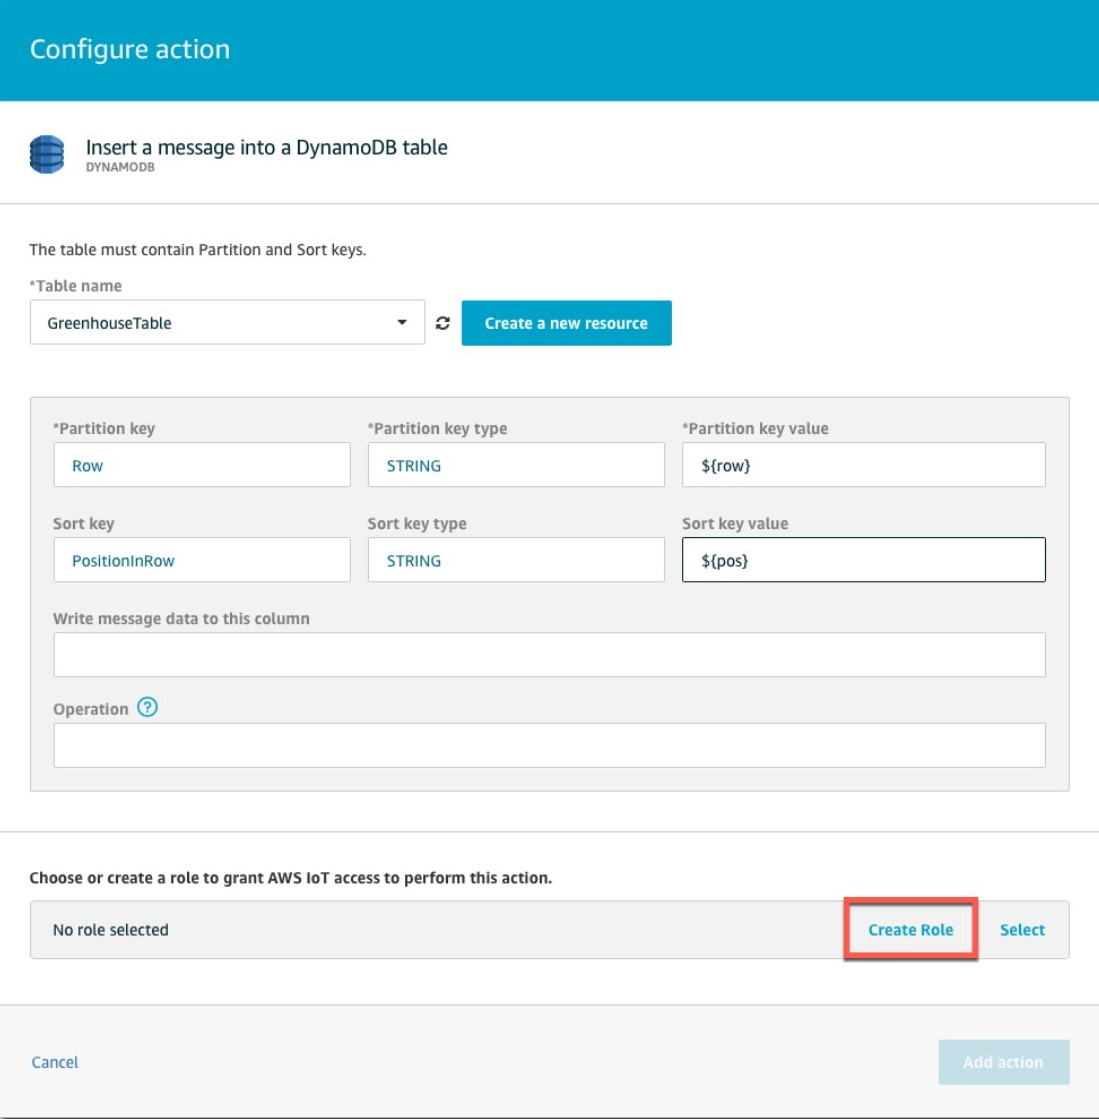
\includegraphics[width=0.41\columnwidth]{images/dynamodb_5}
	\end{center}
	\caption{Creazione di un nuovo ruolo}
	\label{fig:dynamodb_5}
\end{figure}

\subsubsection{Test della Comunicazione}
L'infrastuttura di DynamoDB è stata in questo modo creata e collegata ad IoT Core ed è quindi possibile testare la comunicazione tra AWS IoT Core e DynamoDB per verificare che nel momento in cui IoT Core riceva una nuova entry, questa venga automaticamente inviata alla tabella di DynamoDB che è stata in precedenza collegata. \\
Per fare questo bisogna recarsi nella sezione \textit{Test} e selezionare \textit{Pubblica in un Topic} e nella sezione topic immettere \textbf{EU\_WEST\_2} (lo stesso topic sul quale è in ascolto la regola precedentemente creata \autoref{fig:dynamodb_3}) e nell'area messaggio inserire un nuovo messaggio in formato JSON:
\begin{lstlisting}[language=Java, label= code:JSON_message, caption=Esempio di un possibile messaggio in formato JSON da salvare nel database]
	{
	  "row" : "0",
	  "pos" : "0",
	  "moisture" : "75"
	}
\end{lstlisting}
Quindi cliccare sul pulsante \textit{Pubblica nell'argomento} per inviare il messaggio a tutti i subscriber che sono in ascolto sul topic \textbf{EU\_WEST\_2}, tra i quali la regola di DynamoDB.\\
Infine, per verificare che la regola stia funzionando, accedere alla console di DynamoDB e nella sezione \textit{Tabelle}, cercare la tabella che è stata creata in precedenza e collegata alla regola. Si dovrà quindi vedere la nuova entry all'interno della tabella contenete proprio il messaggio appena pubblicato nel topic.\\
\begin{figure}
	\begin{center}
		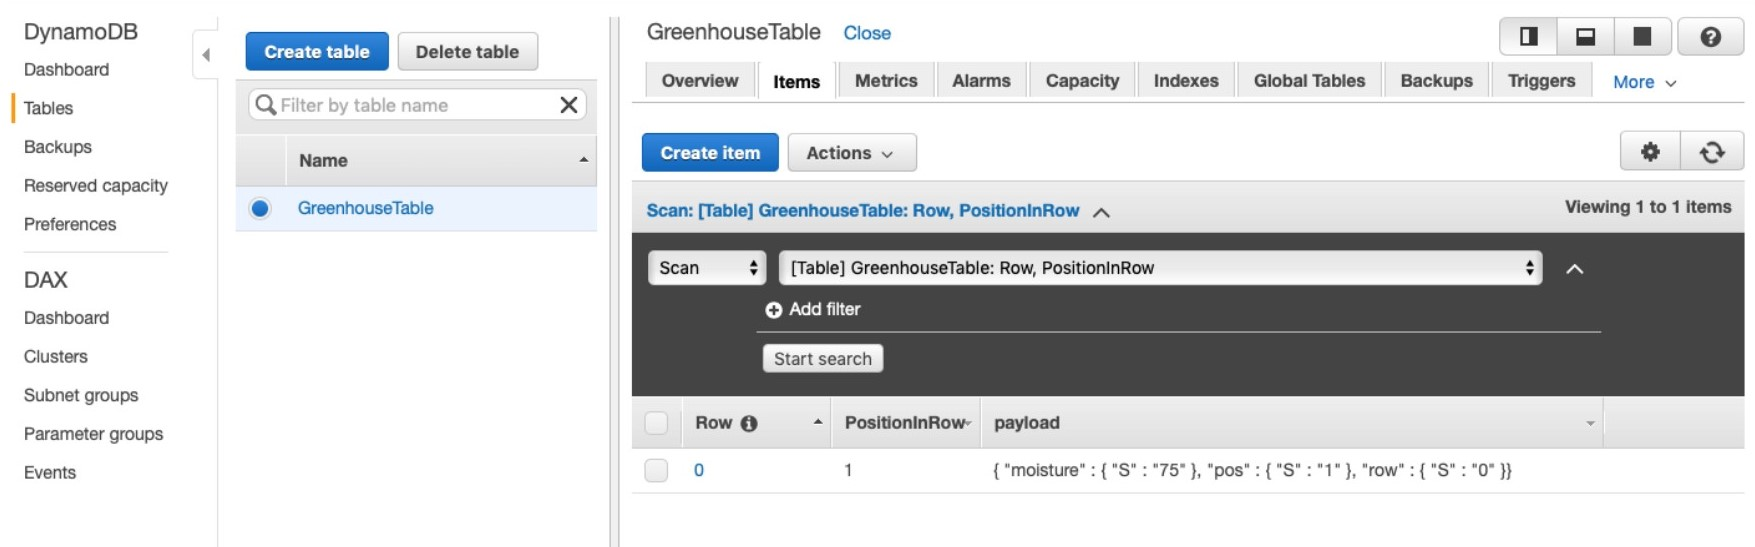
\includegraphics[width=1\columnwidth]{images/dynamodb_6}
	\end{center}
	\caption{Visualizzazione della nuova entry nella tabella}
	\label{fig:dynamodb_6}
\end{figure}
Si noti come, anche in questo caso \autoref{fig:dynamodb_6} si è utilizzato il topic \textbf{EU\_WEST\_2}, lo stesso utilizzato anche nella \autoref{subsubsec:com}. Sebbene il motivo per cui il nome del topic scelto è proprio \textbf{EU\_WEST\_2} sarà esplicitato in dettaglio nella \autoref{sec:aws_core}, per ora basti sapere che, questo stesso set-up della configurazione resta valido e funzionante con qualsiasi altro nome assegnato al topic, purchè i nomi lato Client, Server e lato Databse corrispondano.


\chapter{Implementazione del Sistema}
\label{chap:quattro}
\definecolor{mypink}{RGB}{255, 1, 253}
In questo modo è stata conclusa la fase di progettazione di tutte le componenti del sistema per lo sviluppo di una infrastruttura software che consenta a dispositivi IoT collegati alla rete di poter:
\begin{itemize}
	\item Effettuare delle letture con i sensori ed elaborare questi dati
	\item Stabilire una comunicazione con una piattaforma Cloud opportunamente progettata
	\item Scambiare i dati con la piattaforma Cloud seguendo un protocollo di comunicazione leggero (MQTT) ed uno standard di comunicazione noto (DATEX II)
	\item Conservare automaticamente i dati all'interno di un Database Non Relazione 
	\item Rendere i dati disponibili a query ed analisi dei dati
\end{itemize}
Questi step implementativi che si sono progettati, non sono esclusivi del sistema sviluppato in questo lavoro di tesi, ma sono comuni a moltissime applicazioni del mondo IoT che condividono queste necessità. Pertanto, nel \autoref{chap:tre}, si è cercato di mantenere un basso livello di dettaglio implementativo, proprio per consentire di riutillzare la fase di progettazione mostrata anche in molte altre applicazioni legate al mondo dell'IoT.\\
In questo capitolo, sulla base della progettazione effettuata, si procederà all'implementazione di tutte le componenti e quindi si raggiungerà un maggiore livello di dettaglio attorno ad alcune tecnologie e linguaggi di programmazione. Nella fattispecie, saranno utilizzati:
\begin{itemize}
	\item Linguaggi di Programmazione
	\begin{itemize}
		\item Java
		\item SQL
		\item XML
		\item JSON
	\end{itemize}
	\item Software
	\begin{itemize}
		\item Android Studio
		\item Visual Studio Code
	\end{itemize}
	\item Tecnologie
	\begin{itemize}
		\item Smartphone Android
		\item Amazon Web Services
	\end{itemize}
\end{itemize}
Seguendo il processo logico utilizzato nel \autoref{chap:tre}, al fine di rendere più chiara l'implementazione del software, si continuerà ad utilizzare il Processo Unificato per la documentazione del Software in fase di sviluppo. Dopo aver visto la tabella dei requisiti nel \autoref{chap:tre} ed il diagramma delle classi relativo all'implementazione dello standard di comunicazione DATEX II nel \autoref{app:a}, viene ora realizzato anche il Diagramma dei Casi d'uso il cui scopo è quello di mostrare gli \textbf{Attori} ed i \textbf{Casi d'Uso} e le relazioni tra di essi. Per \textbf{Attore} si intende un qualsiasi utente o servizio esterno al software e per \textbf{Casi d'Uso} si indica una funzionalità del software.\\
\begin{figure}
	\begin{center}
		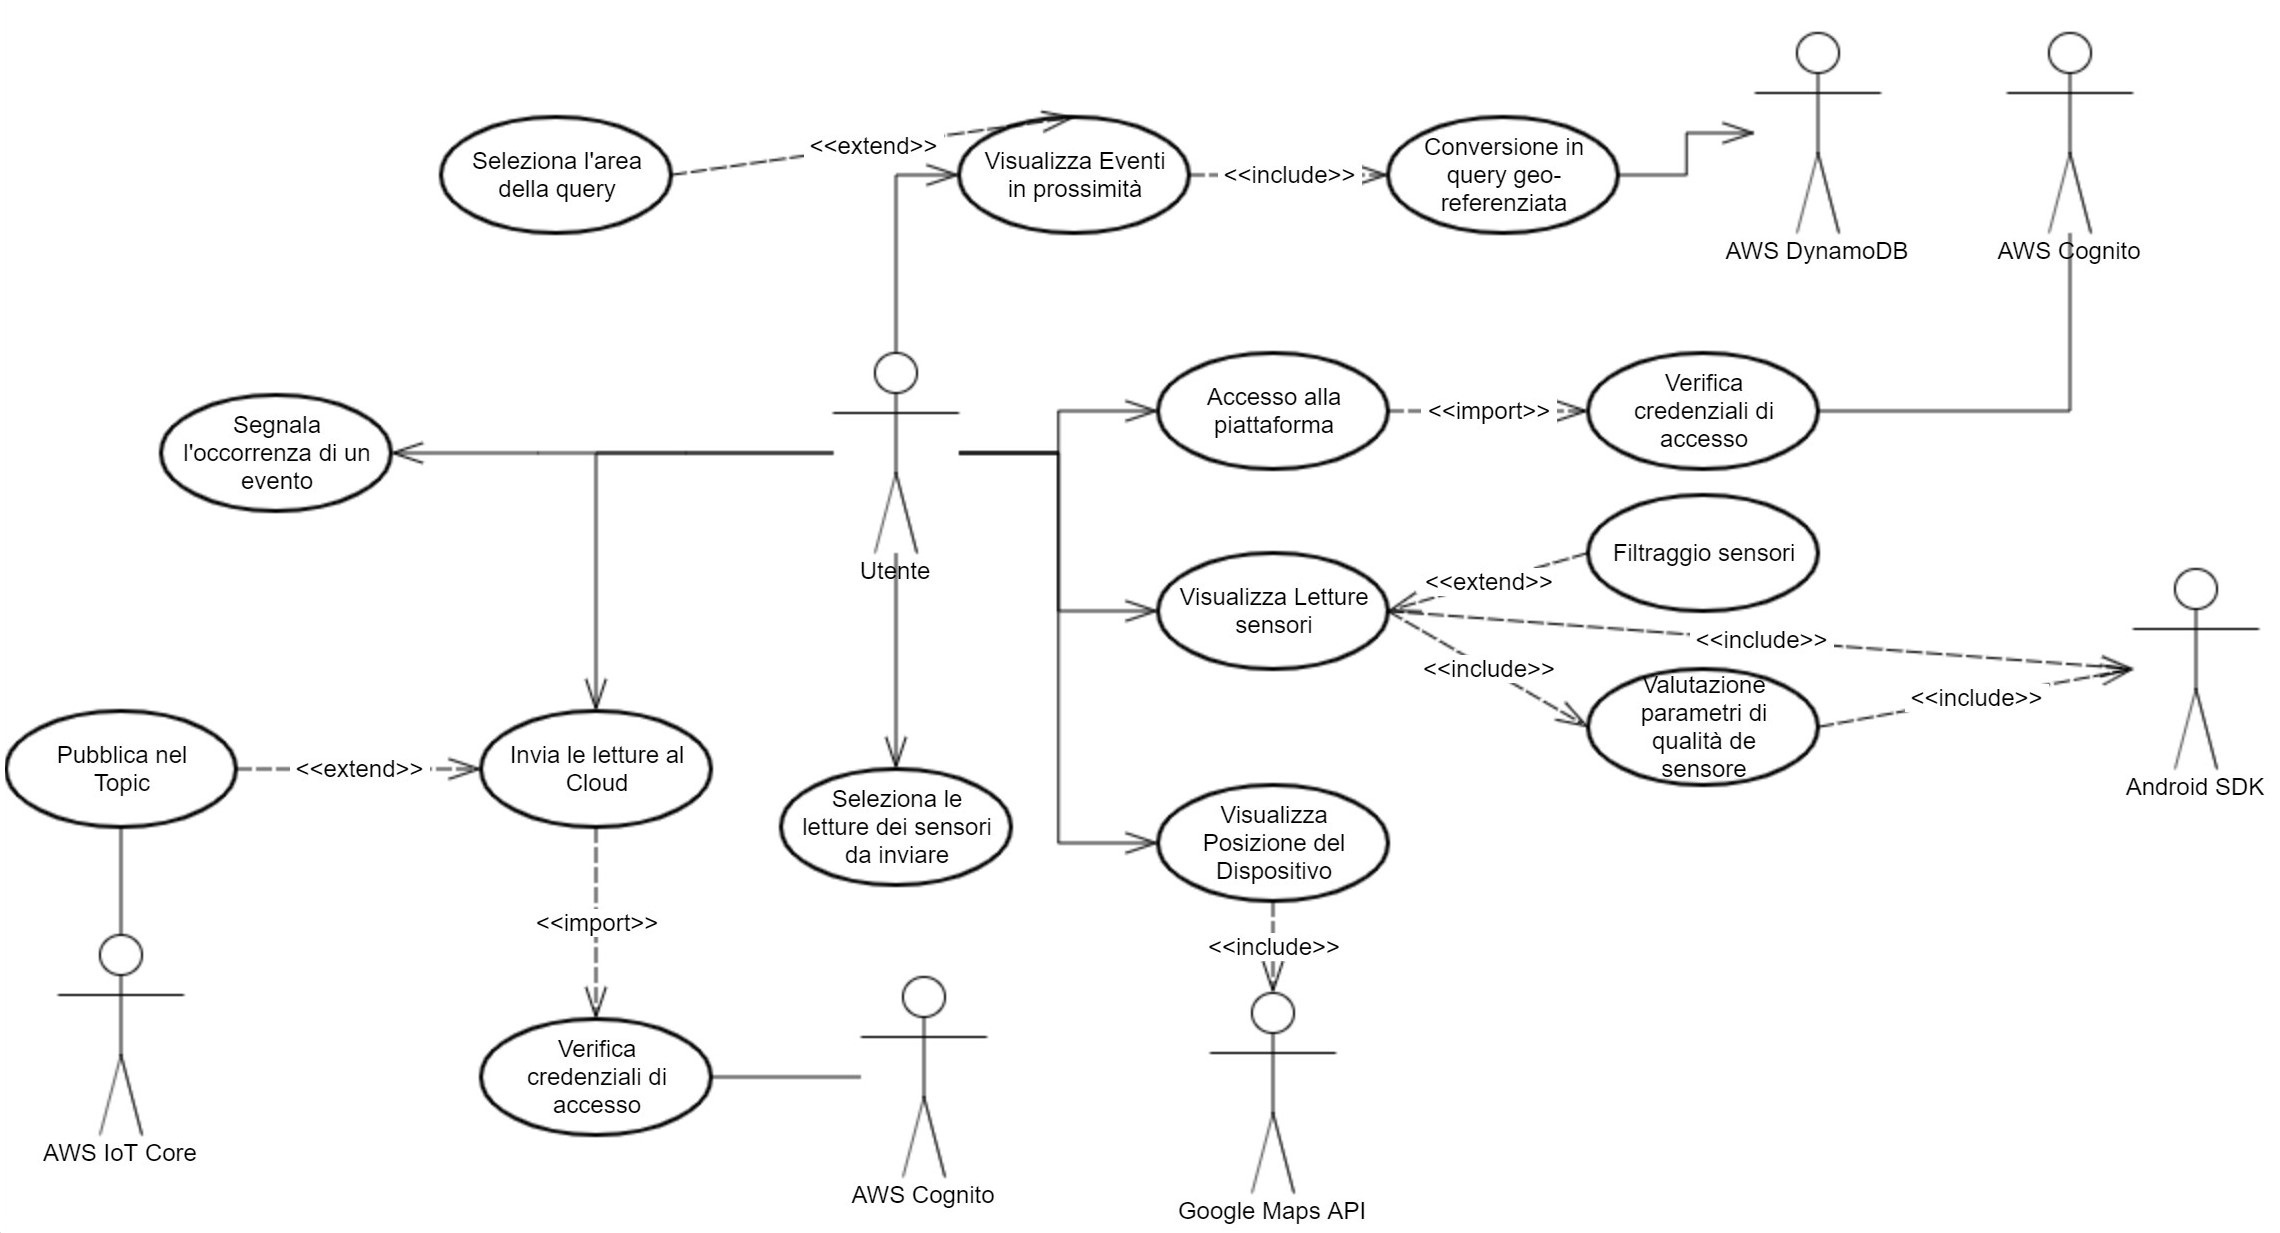
\includegraphics[width=1\columnwidth]{images/casiuso}
	\end{center}
	\caption{Diagramma dei casi d'uso elaborato sulla base dei requisiti funzionali del sistema \autoref{tabel:requisiti_software}}
	\label{fig:casiuso}
\end{figure}
Si procederà quindi per step all'implementazione delle singole componenti del sistema e nella fattispecie, l'ordine implementativo che sarà seguito è:
\begin{enumerate}
	\item Sviluppo della applicazione Android
	\item Sviluppo del Middleware IoT utilizzando la piattaforma AWS IoT Core
	\item Sviluppo delle tabelle nel Database AWS DynamoDB
\end{enumerate}

\section{Applicazione Android}
Per lo sviluppo della applicazione Android, si è scelto di utilizzare l'IDE Android Studio ed il linguaggio di programmazione JAVA. Di seguito, pertanto, utilizzando queste tecnologie saranno implementate le singole componenti della applicazione. Nella fattispecie, la struttura che si vuole dare alla Applicazione Andorid è mostrata in \autoref{fig:android_app_schema}.
In Android, ciascuna pagina di una applicazione Android contenente un riferimento al layout da mostrare all'utente ed un riferimento al codice JAVA associato alla pagina è chiamata Activity. Invece, un servizio utilizzato all'interno di una Activity viene chiamato Modulo. Ciascun modulo assolverà ad uno specifico compito. Pertanto, prima di passare alla implementazione di ogni Activity e Modulo della applicazione, si progetti lo schema generale che i vuole implementare.\\
\begin{figure}
	\begin{center}
		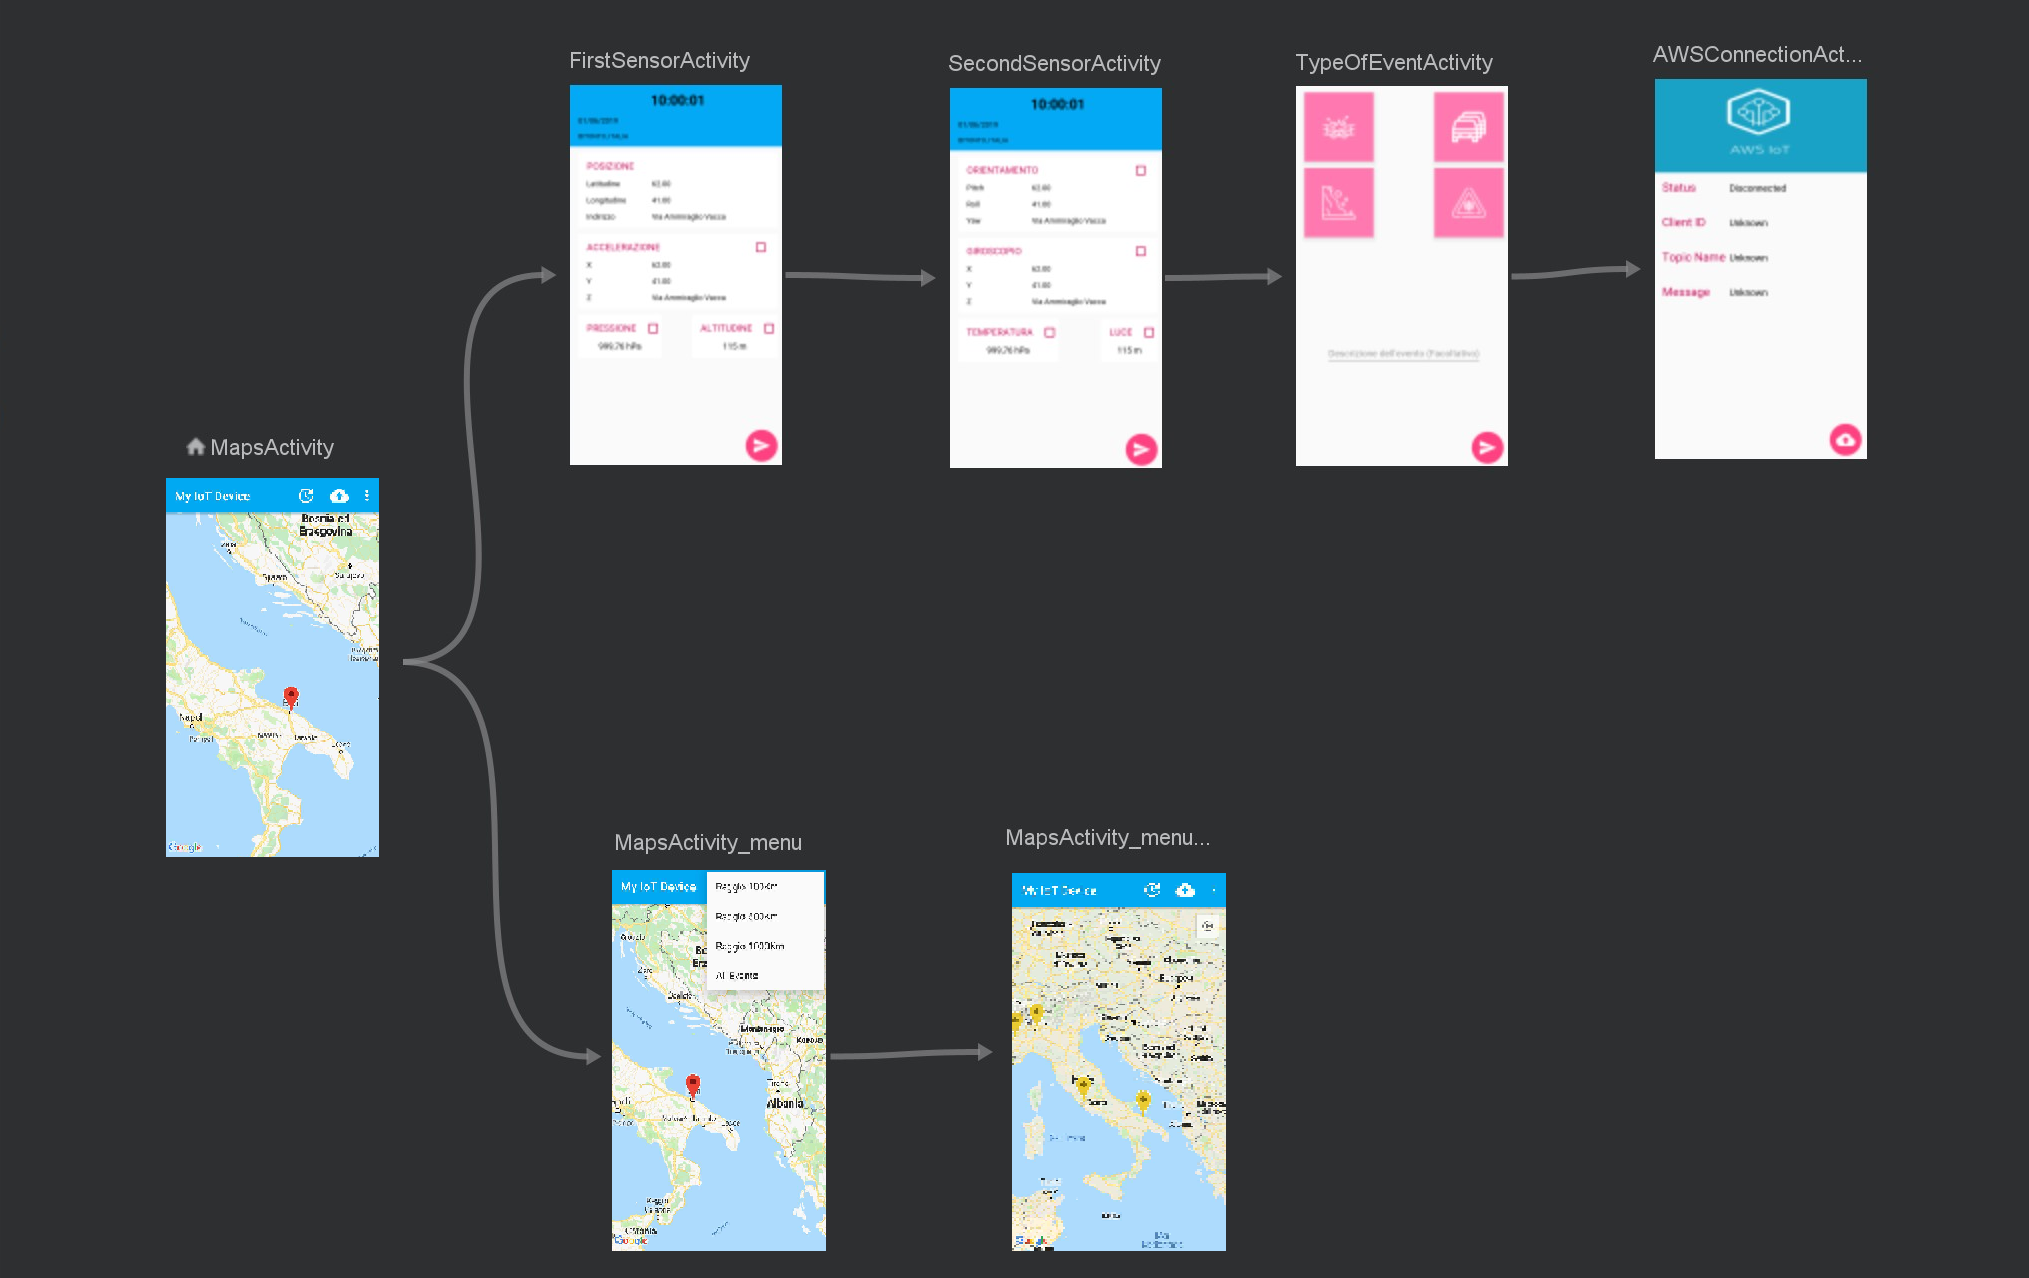
\includegraphics[width=1\columnwidth]{images/android_app_schema}
	\end{center}
	\caption{Schema delle Activity che compongono la applicazione Android}
	\label{fig:android_app_schema}
\end{figure}
\begin{figure}
	\begin{center}
		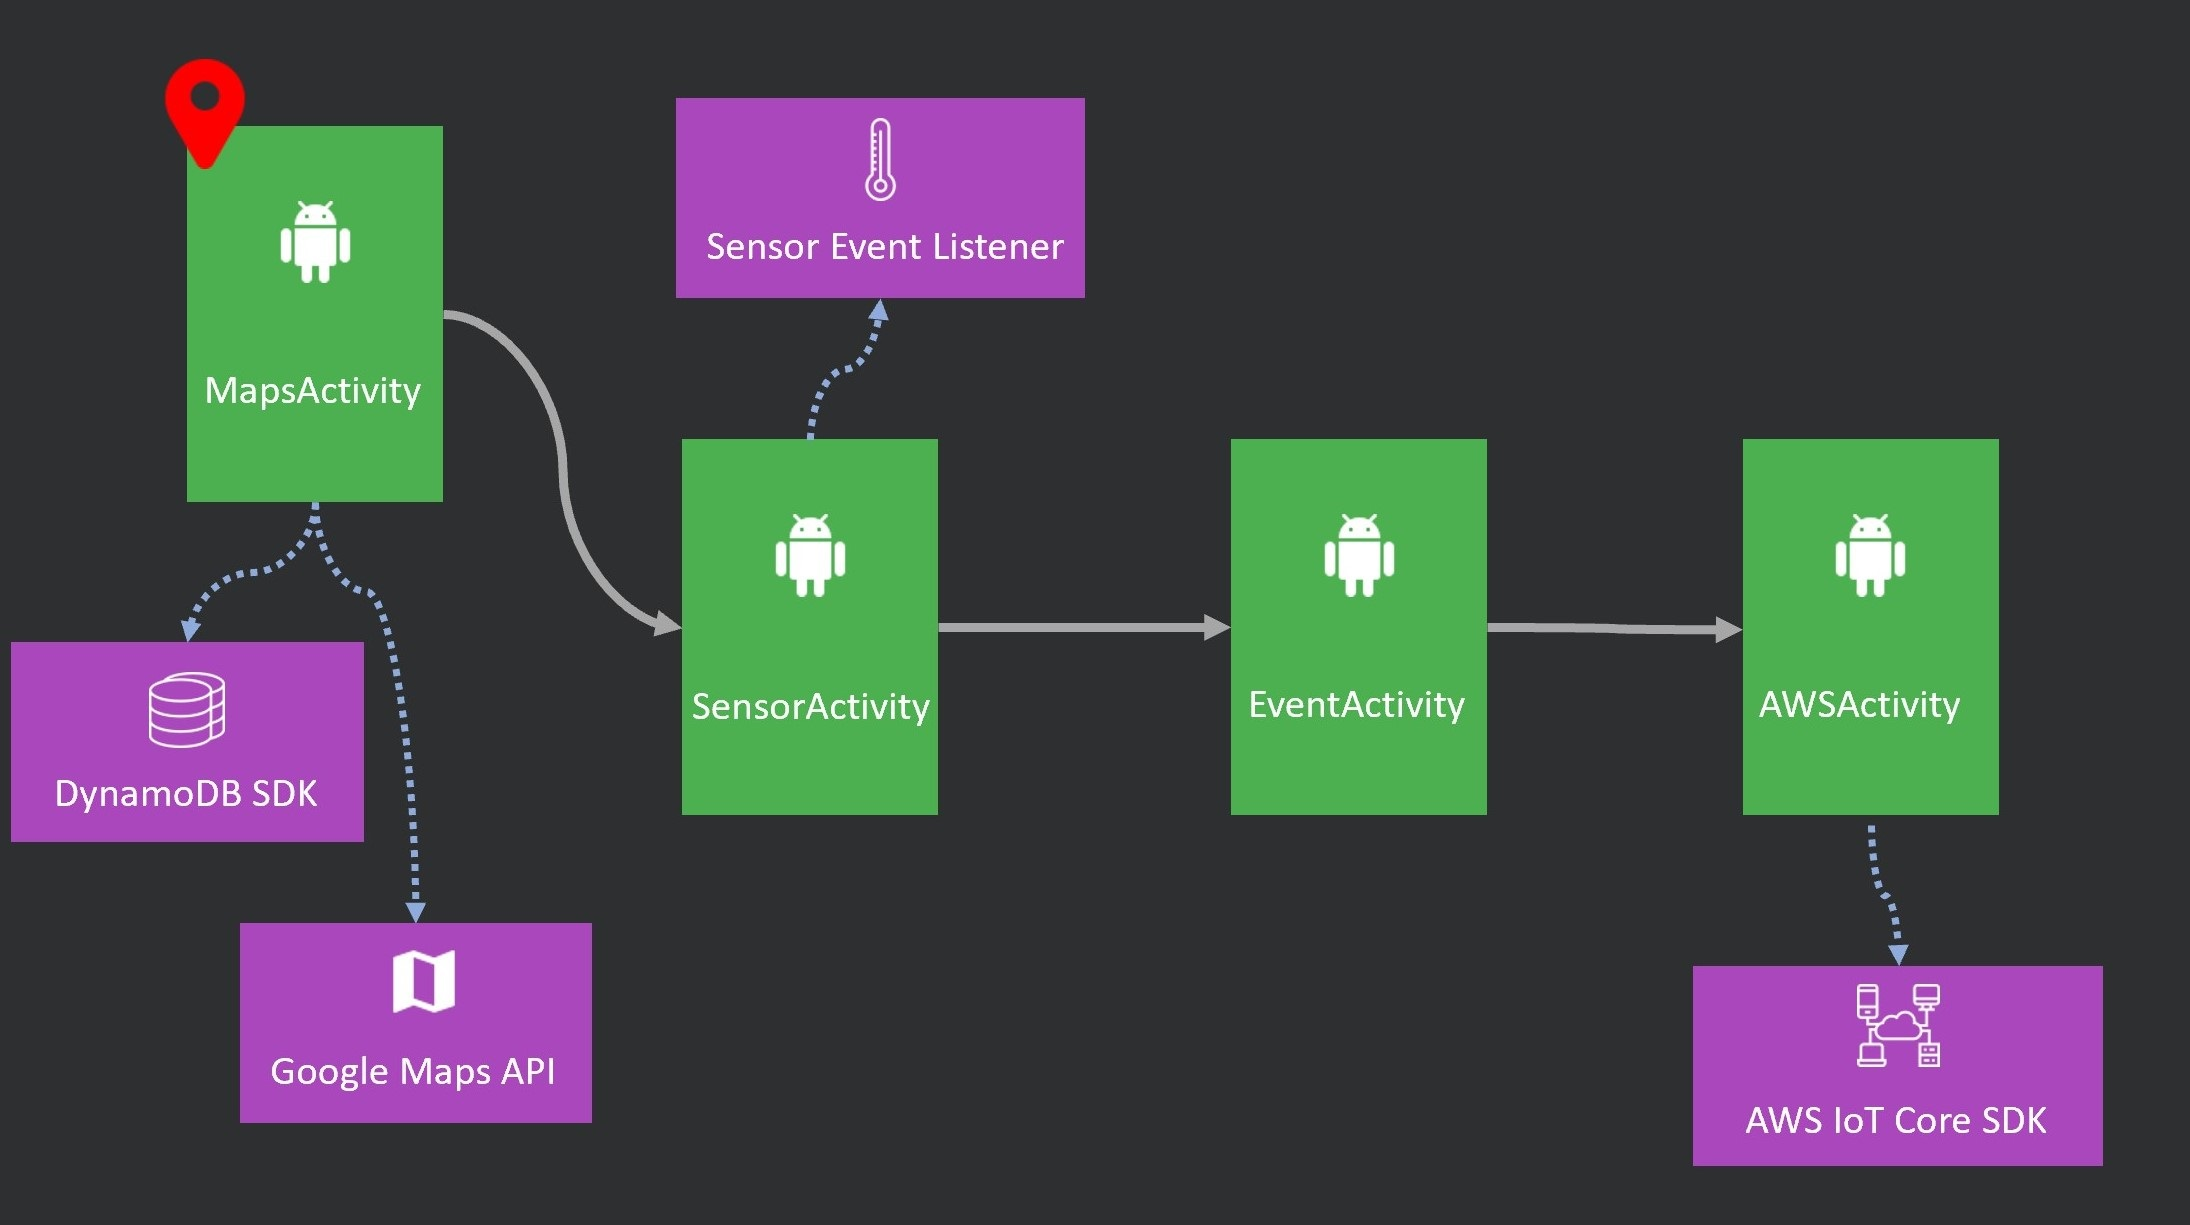
\includegraphics[width=0.9\columnwidth]{images/android_app_schema_1}
	\end{center}
	\caption{Moduli utilizzati da ciascuna Activity}
	\label{fig:android_app_schema_1}
\end{figure}
Dal momento che si è decsio di utilizzare l' IDE Android Studio, si proceda con la creazione di un nuovo progetto che quindi produrrà automaticamente lo schema della applicazione. Questo sarà lo scheletro della applicazione dal quale partire con l'implementazione di tutte le Activity ed i Moduli \autoref{fig:android_app}.
\begin{figure}
	\begin{center}
		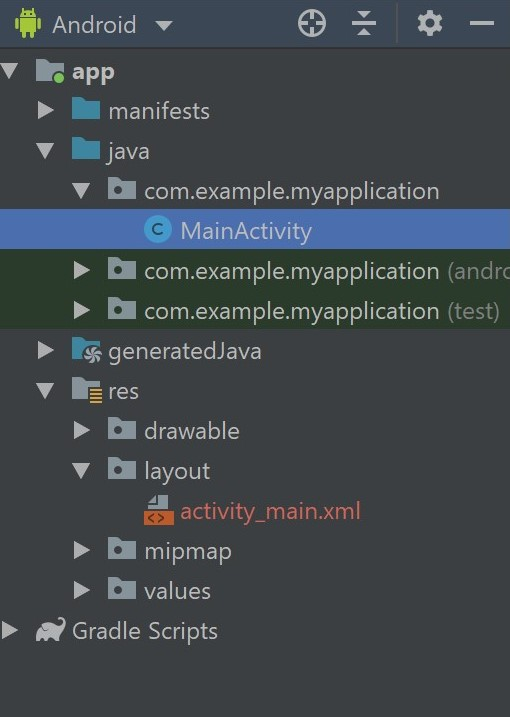
\includegraphics[width=0.3\columnwidth]{images/android_app}
	\end{center}
	\caption{Overview della nuova directory creata da Android Studio}
	\label{fig:android_app}
\end{figure}
Sono quindi mostrate nelle sezioni successive tutte le Activity che compongono la applicazione ed i rispettivi Moduli utilizzati.

\subsection{MapsActivity}
La MainActivity è quella che Android definisce come punto di partenza per il bootstrap o avvio di tutta la Applicazione. In questo caso, si vuole fare in modo che la prima Activity da mostrare all'utente sia la MapsActivity.\\
Lo scopo di questa Activity è quello di mostrare a schermo una mappa e, sfruttando la localizzazione GPS dello smartphone, di mostrare la posizione in tempo reale dell'utente sulla stessa mappa.\\
Ulteriormente, in questa Activity è necessario dare la possibilità all'utente di recuparare gli eventi conservati in una tabella di un Database DynamoDB (\autoref{fig:maps_activity}) attraverso una query geo-referenziata \textcolor{mypink}{1} e di mostrarli nella mappa attraverso dei marker \textcolor{mypink}{2}. Inoltre, accedendo al menù \textcolor{mypink}{3}, l'utente è in grado di modificare l'area degli eventi da recuperare dal Database.
\begin{figure}%
	\centering
	\subfloat[Componenti della MapsActivity]{{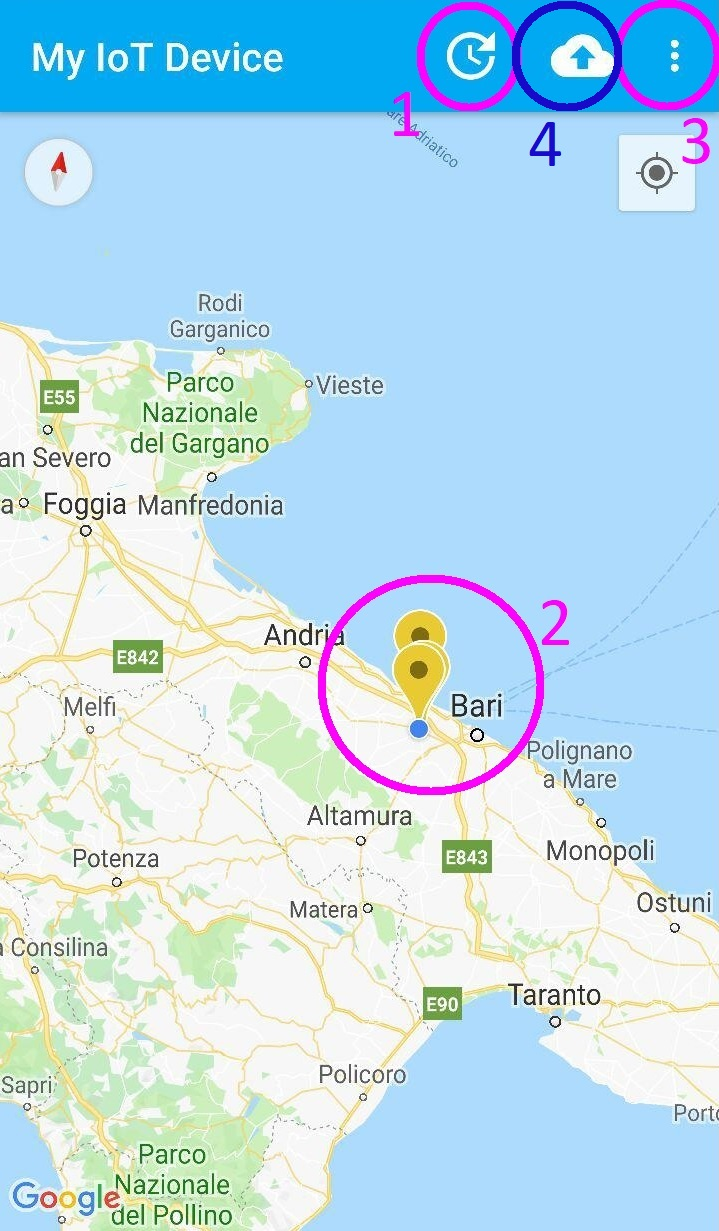
\includegraphics[width=5cm]{images/maps_activity_1} }}%
	\qquad
	\subfloat[Dettaglio del menù a tendina mostrato al click sul pulsante 3]{{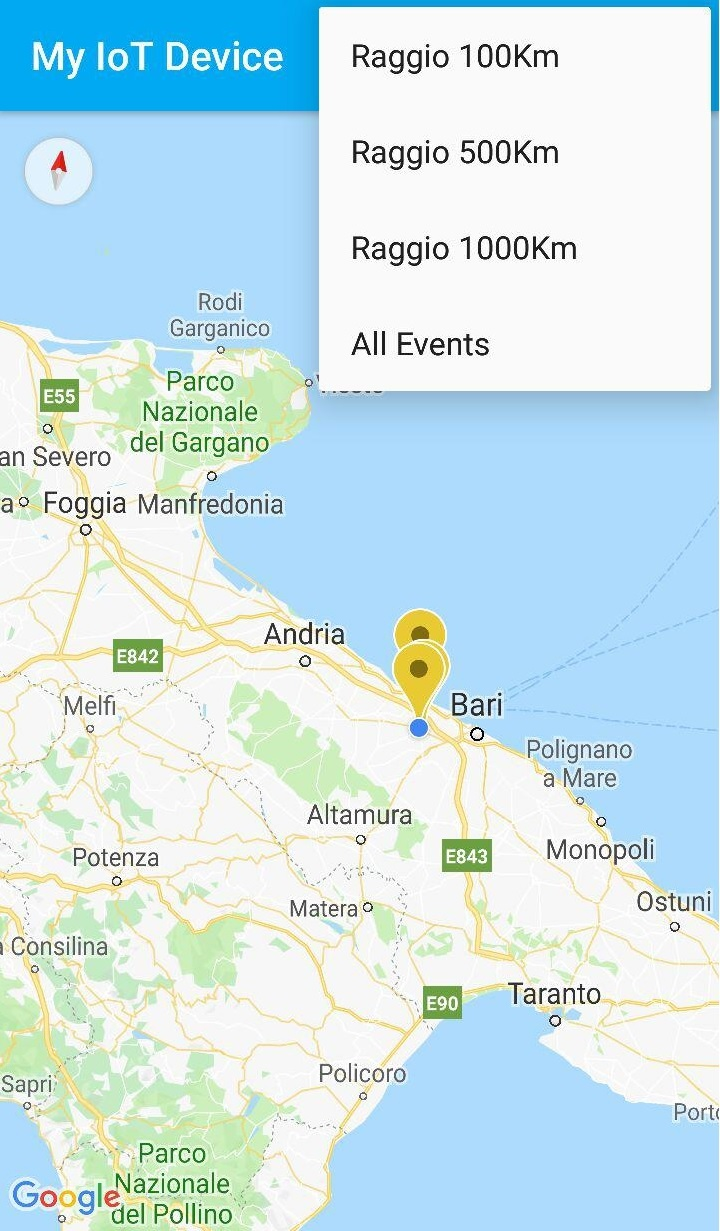
\includegraphics[width=5cm]{images/maps_activity_2} }}%
	\caption{Layout della Activity inziale nell'applicazione Android}%
	\label{fig:maps_activity}%
\end{figure}
In dettaglio, ad un click sul pulsante \textcolor{mypink}{3}, viene mostrato il menù a tendina che consente all'untente di selezionare la dimensione della query da inoltrare al Database.\\
Invece, un click sul pulsante \textcolor{blue}{4} consentirà all'utente di navigare verso le altre Activities che compongono la applicazione Android e nella fattispecie verso la SensorActivity che mostrerà a schermo le letture dei sensori dei quali lo smartphone è provvisto in real-time.\\
Di seguito, sono sposti gli step implementativi necessari alla realizzazione di questa Activity. Il codice relativo al layout di ciascuna applicazione è stato omesso in quanto non influisce direttamente sulle funzionalità implementate dalla applicazione stessa ed è ritenuto pertanto superfluo.

\subsubsection{Option Menu}
Per la creazione di un menù a tendina e per la conseguente gestione dei click sullo stesso è necessario:
\begin{itemize}
	\item \textit{Creare un nuovo layout del menu:} nella cartella \textbf{res} si crei una nuova cartella \textbf{menu} ed un nuovo file XML al suo interno. Questo file XML appena creato dovrà contenere il layout del menù a tendina da mostrare.
	
	\item \textit{Creare la MapsActivity.java ed associare i layout:} Nella cartella\\ \textbf{java/com.example.myapplication} si crei una nuova Activity che mostri a schermo il layout della mappa e quello del menu.
	\lstinputlisting[caption=Mostro a schermo il layout che ospiterà la mappa]{code/maps_activity_1.java}
	
	\item \textit{Gestire le interazioni dell'utente con il Menu:} Si rende necessario predisporre un listener in ascolto di eventuali iterazioni dell'utente con gli elementi del menù a tendina. In tal modo, al click su uno dei pulsanti del menù, si andrà ad aggiornare il valore dell'area della query e conseguentemente la query al database verrà reinviata per soddisfare le nuove richieste.
	\lstinputlisting[caption=Listener associato agli elementi del Menu]{code/maps_activity_2.java}
\end{itemize}

\subsubsection{GPS e Google Maps API}
Una volta creato il layout della applicazione, si implementi ora la componente che consente alla Activity di mostrare a schermo la posizione dell'utente nella mappa. Questa componente utilizzerà la posizione GPS dello smartphon per aggiornare in tempo reale una mappa. Inoltre, al fine di mostrare correttamente la mappa, è necessario sfruttare le API messe a disposizione da Google Maps.
\begin{itemize}
	\item \textit{Richiesta delle permission all'utente:} Si richiede all'utente il permesso di accedere alla posizione GPS ed alla connessione Internet del suo dispositivo. Il GPS sarà utilizzato per la posizione in real-time e la connessione ad internet sarà utilizzata per mostrare la Mappa.
	\lstinputlisting[caption=Accesso al GPS e connessione Internet]{code/permission.java}
	
	\item \textit{Utilizzo delle Google Maps API:} Al fine di mostrare a schermo una mappa è necessario ottenere una chiave API da Google Maps, previa registrazione al Web Service. Va pertanto creato un nuovo documento XML nella directory \textbf{res/google\_maps\_api.xml} e segire le istruzioni in \url{https://developers.google.com/maps/documentation/android/start#get-key} per ottenere una nuova chiave. Questa chiave andrà poi inserita all'interno del file XML appena creato.
	\lstinputlisting[caption=Utilizzo della chiave fornita da Google Maps per l'utilizzo delle Mappe]{code/google_map_api.xml}
		
	\item \textit{Aggiornamento in real time della view:} Sfruttando la posizione GPS e le Google Maps API, viene aggiornata in real-time la posizione dell'utente sulla mappa.
\end{itemize}

\subsubsection{Query del Database}
Infine, è necessario gestire le query da inviare al Database DynamoDB. Infatti, in funzione della scelta dell'utente sulla dimensione del raggio della query, verranno formulate delle query geo-referenziate al Database DynamoDB in modo da raccogliere i soli eventi segnalati nell'area prescelta.
\begin{itemize}
	\item \textit{Utilizzo l'SDK di DynamoDB:  }Viene sfruttato l'SDK messo a disposizione da AWS DynamoDB per mappare i dati contenuti nelle tabelle del database, sottoforma di classe all'interno dell'applicazione Android.
	\lstinputlisting[caption=Mapping delle tabelle ed attributi del Database DynamoDB che si vuole mappare]{code/dynamodb_3.java}
	
	\item \textit{Creazione di un task asincrono:} Viene utilizzato un task asincrono per l'interrogazione del database in modo da consentire all'utente di continuare ad usare l'interfaccia grafica anche durante le interrogazioni del Database.
	\lstinputlisting[caption=<struttura del Task Asincrono che dovrà interrogare il Database]{code/dynamodb_8.java}
	
	\item \textit{Composizione della Query:} Dovendo lanciare una query geo-referenziata e, dal momento che i dati nel database sono anch'essi geo-referenziati attraverso i campi latitudine e longitudine, è necessario ora unire le informazioni relative alla latitudie e longitudine corrente dell'utente con quelle relative al raggio della query. L'obiettivo di questo calcolo  quello di ottenere un intervallo di posizioni accettabili. Queste saranno caratterizzate dall'avere una latitudine e longitudine comprese all'interno di un certo intervallo.
	\lstinputlisting[caption=Calcolo dei parametri con i quali inviare una query geo-referenziata]{code/dynamodb_4.java}
	
	\item \textit{Invio della query geo-referenziata:} Sulla base del mapping effettuato tra gli attributi della tabella di DynamoDB e l'applicazione android, si può ora lanciare la query ed applicare il filtro sull'intervallo di posizioni che si vogliono raccogliere.
	\lstinputlisting[caption=Composizione ed invio della query]{code/dynamodb_5.java}
\end{itemize}

\subsubsection{Creazione di Marker sulla Mappa}
Una volta effettuata la query al Database DynamoDB, è necessario predisporre la ricezione della lista di tutti gli elementi che rispettano i parametri della query, decodificarli dal formato JSON nel quale sono trasmessi ad un formato più user-friendly e conseguentemente mostrarli a schermo sottoforma di marker nella mappa.
\begin{itemize}
	\item \textit{Ricevo la Lista di messaggi:} Inviata la query, mi aspetto di ricevere una lista di messaggi da parte del Database DynamoDB corrispondenti agli elementi all'interno del Database che soddisfano la query. 
	\lstinputlisting[caption=Ricezione degli item che soddisfano la query]{code/dynamodb_6.java}
	
	\item \textit{Creo un marker per ogni evento:} Ogni elemento ricevuto corrisponderà ad un evento geo-referenziato contenuto nel Database. Uso gli attributi latitudine e longitudine dell'evento per mostrarlo nella Mappa precedentemente creata.
	\lstinputlisting[caption=Visualizzazione di ciascun evento come marker sulla mappa]{code/dynamodb_7.java}
\end{itemize}

\subsection{SensorActivity}
La SensorActivity viene attivata ad un click dell'utente sul pulsante \textcolor{blue}{4} della \autoref{fig:maps_activity}. Lo scopo di questa Activity è quello di mostrare a schermo una panoramica delle letture restituite da tutti i sensori di cui è dotato lo smartphone per sottoporle ad una revisione dell'utente al fine di decidere quali di queste letture inviare al Server per le successive analisi. 
Dal momento che il panorama degli smartphone è notoriamente frammentato in termini di dotazione software ed hardware, si è deciso di predisporre una view per ogni sensore che potrebbe risultare utile alle successive analisi dei dati. Nella fattispecie, i sensori per cui sono stati predisposti i metodi necessari alla raccolta e visualizzazione dei dati sono:
\begin{itemize}
	\item Accelerazione
	\item Pressione Atmosferica
	\item Altimetro
	\item Orientamento
	\item Giroscopio
	\item Temperatura
	\item Intensità Luminosa
\end{itemize}
A prescindere dalla dotazione del dispositivo, si predisporranno i metodi utili ad ottenere le letture di questi sensori ove presenti. In caso uno dei sensori sopra citati dovesse non essere in dotazione dello smartphone, non ne sarà data alcuna lettura.
\begin{figure}%
	\centering
	\subfloat{{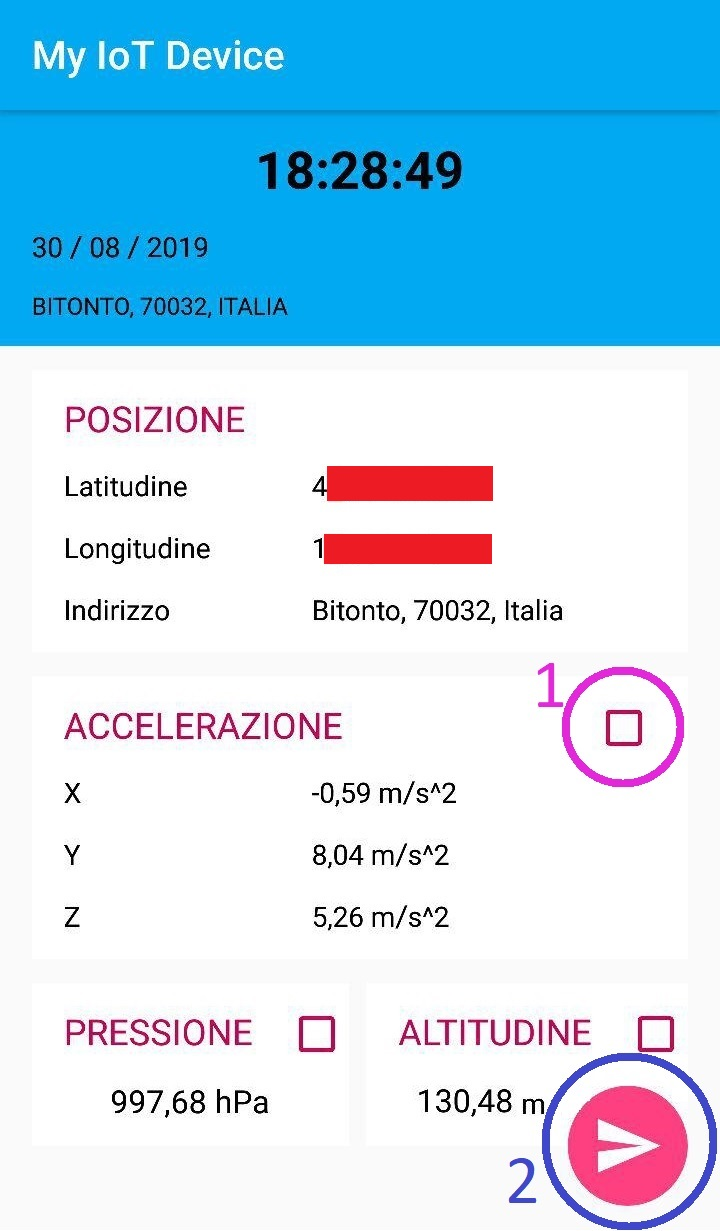
\includegraphics[width=5cm]{images/sensor_activity_1} }}%
	\qquad
	\subfloat{{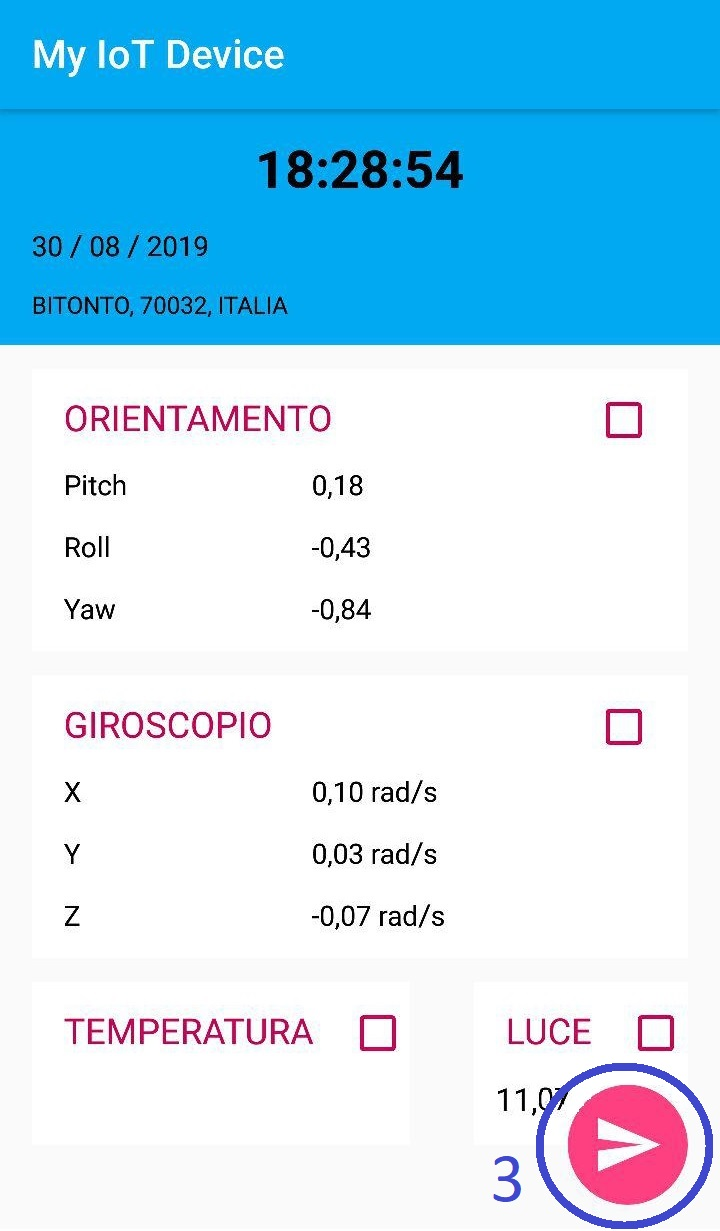
\includegraphics[width=5cm]{images/sensor_activity_2} }}%
	\caption{Lista Sensori con le relative misure}%
	\label{fig:sensor_activity}%
\end{figure}
Un click da parte dell'utente sulla CheckBox \textcolor{mypink}{1} consentrà di selezionare la lettura del relativo sensore da inviare al Middleware IoT. Cliccando invece sul FloatingButton \textcolor{blue}{2} si navigherà ad una SensorActivity gemella che mostrerà le letture di altri sensori. Infine, un click sul pulsante \textcolor{blue}{3}, farà navigare l'utente verso la Activity successiva (EventActivity).\\
Di seguito sono mostrati gli step per la visualizzazione dei dati di ciascun sensore. A titolo di esempio, questi step saranno mostrati per l'accelerometro ma potranno essere ripetuti per tutti gli altri sensori.
\begin{itemize}
	\item \textit{Creazione di un riferimento al SensorManager:} Al fine di ottenere l'accesso alle letture dei sensori, è necessario sfruttare un Modulo messo a disposizione dal framework Android chiamato SensorManager. Il SensorManager, si occuperà di disabilitare i sensori non necessari, specialmente quando la Activity è in pausa. Questo perchè il sistema non disattiva automaticamente i sensori quando lo schermo viene spento ne quando l'Activity viene messa in pausa e ciò si tradurrebbe in un eccessivo consumo della batteria.
	\lstinputlisting[caption=Creazione del riferimento al SensorManager che sarà condiviso tra tutti i sensori mostrati nella Activity]{code/sensor_1.java}
	
	\item \textit{Accesso alle risorse dello Smartphone:} Per ogni sensore che si intende utilizzare è necessario recuperare un riferimento al particolare sensore attraverso il SensorManager precedentemente istanzaiato. I diversi Sensori presenti all'interno di uno smartphone sono indivisuati dal SensorManager attraverso una lista di costanti accessibili da : \url{https://developer.android.com/guide/topics/sensors/sensors_overview}. In questo caso, si crei il riferimento all'accelerometro.
	\lstinputlisting{code/sensor_2.java}
	
	\item \textit{Creazione di un Thread separato:} Al fine di gestire le letture provenienti dal sensore e poterle inoltrare all'utente nella SensorActivity, è necessario creare un Thread separato rispetto a quello sul quale viene eseguita la SensorActivity. In questo modo, la SensorActivity sarà ancora disponibile all'utilizzo mentre un thread parallelo si starà procurando le letture dei sensori.
	\lstinputlisting[caption=Creazione e lancio del thread separato che leggerà i valori dall'accelerometro.]{code/sensor_3.java}
	
	\item \textit{Registrazione di un Listener sul Thread separato:} Al fine di recuperare e trattare i dati provenienti dal thread appena creato per l'accelerometro, è necessario creare e registrare un listener il cui compito è quello di eseguire delle operazioni sulle letture del sensore, nonappena sono ricevuti dei nuovi dati dal sensore stesso.
	\lstinputlisting[caption=Registrazione del Listener sull'accelerometro.]{code/sensor_4.java}
	\lstinputlisting[caption=Modulo Sensor Event Listener.]{code/sensor_5.java}
	
	\item \textit{Filtraggio dei dati in uscita dall'accelerometro:} Come evidenziato nella \autoref{subsec:filtering_sensor}, è necessario effettuare il filtraggio delle letture provenienti da alcuni sensori al fine i ottenere delle letture più accurate. L'accelerometro è tra quei sensori Hardware che richiedono un filtraggio dei dati.
	\lstinputlisting[caption=Funzione applicata all'output dell'accelerometro per il filtraggio dei dati con un filtro passa-basso.]{code/sensor_6.java}
	
	\item \textit{Stampa a schermo delle letture del sensore:} Una volta filtrati, i dati sono disponibili ad essere visualizzati nella SensorActivity.
	\lstinputlisting[caption=Accesso al contenuto degli elementi della view nella SensorActivity.]{code/sensor_7.java}
	
	\item \textit{Recupero dei parametri di qualità del sensore:} Per concludere con il processo di lettura dei dati di un sensore, è necessario corredare l'output del sensore con i parametri di qualità del sensore, la cui utilità è stata discussa nella \autoref{subsec:quality_param}.
	\lstinputlisting[caption=Lettura delle caratteristiche salienti del sensore.]{code/sensor_8.java}
\end{itemize}

\subsection{EventActivity}
\label{subsec:event_activity}
La EventActivity viene attivata ad un click dell'utente sul pulsante \textcolor{blue}{3} della \autoref{fig:sensor_activity}. Lo scopo di questa Activity è quello di mostrare a schermo una lista di possibili eventi stradali tra i quali l'utente può scegliere quelli eventualmente occorsi. Qualora infatti uno di questi eventi dovesse verificarsi lungo la rete stradale, l'utente può informare il sistema e di conseguenza tutti gli altri automobilisti dell'eventuale pericolo.
Infine si mette a disposizione anche una label per l'eventuale inserimento di una descrizione dell'evento \textcolor{mypink}{2}. Un click sul pulsante \textcolor{blue}{3} consentirà invece la navigazione verso la Activity successiva (AWSActivity).
\begin{figure}%
	\centering
	\subfloat[Componenti della EventActivity]{{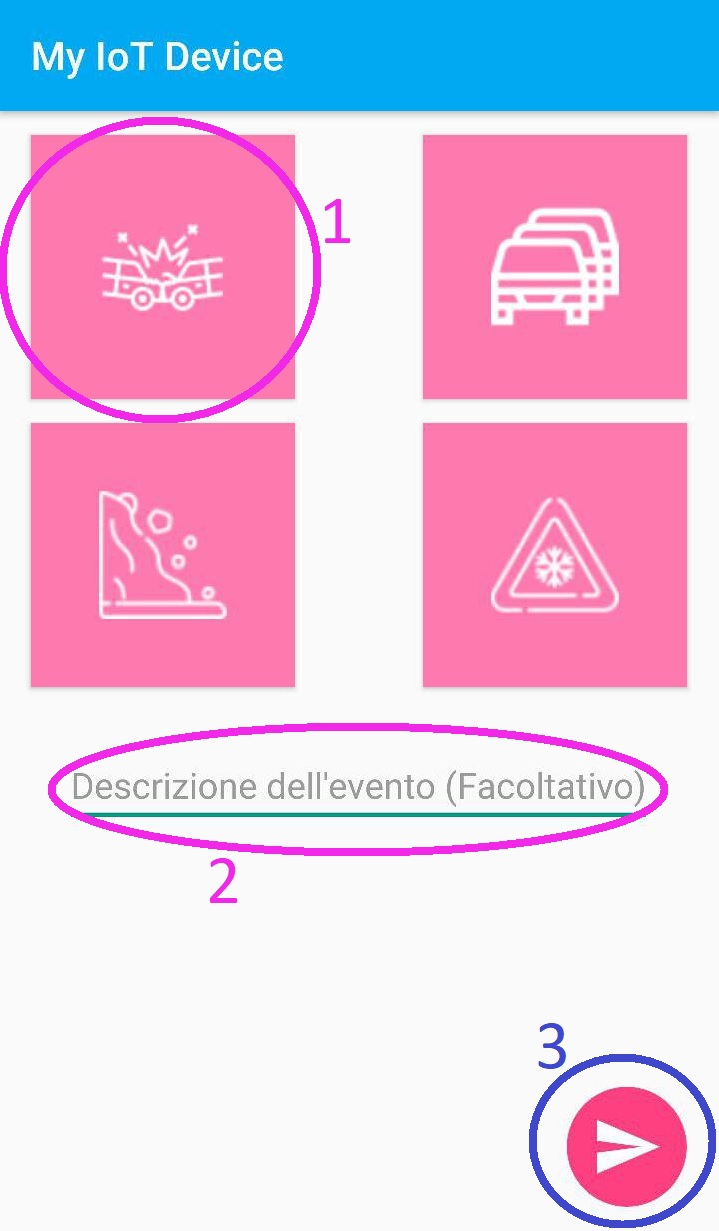
\includegraphics[width=5cm]{images/event_activity_1} }}%
	\qquad
	\subfloat[Dettaglio del click sul pulsante 1]{{\includegraphics[width=5cm]{images/event_activity_2} }}%
	\caption{Layout della EventActivity}%
	\label{fig:event_activity}%
\end{figure}
Considerata la semplicità del contenuto da mostrare a schermo in questa Activity e considerato che questa sarà l'ultima Acivity a raccogliere i dati proposti dall'utente, conseguentemente al click dell'utente sul pulsante \textcolor{blue}{3} si creerà direttamente il payload del pacchetto da inviare nella Activity successiva (AWSActivity) in formato XML ed in formato JSON.\\
Per l'implementazione di queste componenti, sono stati seguiti gli step seguenti:
\begin{itemize}
	\item \textit{Gestire i click sui Pulsanti:} Per ciscun pulsante corrispondente ad un possibile evento stradale, viene predisposto un Listener che quindi resti in ascolto di interazioni con l'utente e si comporti di conseguenza.
	\lstinputlisting[caption=Gestione del click sul primo pulsante.]{code/event_1.java}
	
	\item \textit{Creazione della Publication in DATEX II:} In accordo con quanto definito dallo standard DATEX II che si è deciso di utilizzare come formato per lo scambio dati relativi al traffico, questi dati raccolti dall'utente saranno impacchettati in una Publication e conseguentemente convertiti in XML e JSON. Questa procedura è eseguita in questa Activity sulla base dello schema delle classi dell' \autoref{app:a} e sulla base dell'implementazione delle stesse evidenziata nell'\autoref{app:b}.
	
	\item \textit{Conversione della Publication in XML e JSON:} Android non prevede dei moduli integrati per la conversione di un oggetto in formato XML, ma solo in formato JSON. Pertanto, la conversione dell'oggetto Publication in formato XML sarà fatta utilizzando una libreria esterna. 
	\lstinputlisting[caption=Utilizzo della libreria XStream per la conversione della publication in formato XML.]{code/event_2.java}
	Per quanto riguarda invece la convesrione in formato JSON, sarà utilizzata la libreria Gson messa a disposizione da Android.
	\lstinputlisting[caption=Utilizzo della libreria Gson per la conversione della Publication in formato JSON.]{code/event_3.java}
\end{itemize}

\subsection{AWSActivity}
\label{subsec:aws_activity}
La AWS Activity viene attivata ad un click dell'utente sul pulsante \textcolor{blue}{3} della \autoref{fig:event_activity}.
\begin{figure}%
	\centering
	\subfloat[Componenti della AWSActivity]{{\includegraphics[width=5cm]{images/aws_activity_1} }}%
	\qquad
	\subfloat[Dettaglio del click sul pulsante 1]{{\includegraphics[width=5cm]{images/aws_activity_2} }}%
	\caption{Layout della AWSActivity}%
	\label{fig:aws_activity}%
\end{figure}
Lo scopo di questa Activity è quello di stabilire una connessione con la piattaforma Cloud AWS IoT Core attraverso un click sul pulsante \textcolor{mypink}{1} e, una volta stabilita la connessione, procedere all'invio del messaggio al Middleware IoT con un click sul pulsante \textcolor{blue}{2}. \\
Le funzionalità associate a questa Activity potrebbero essere tranquillamente incorporate in un click sul pulsante \textcolor{blue}{3} della \autoref{fig:event_activity}. Tuttavia, ai fini della prototipazione, si è scelto di tenere queste funzionalità in una Activity separata in modo da mostrarne in dettaglio le singole operazioni.
La sequenza di operazioni eseguite in questa Activity saranno quindi:
\begin{itemize}
	\item \textit{Set-Up dei parametri necessari alla Connessione:} Al fine di stabilire la connessione con il Server AWS IoT Core, è necessario che ciascun Client sia registrato al servizio Amazon Web Services e che quindi abbia un ID ed una Password per il proprio accesso. In questa fase prototipale, il processo di registrazione è stato fatto manualmente seguendo la procedura esposta nella \autoref{sec:iot_core}. Le credenziali di accesso ottenute in questo processo di registrazione saranno utilizzate per l'autorizzazione della applicazione in fase di sviluppo alla comunicazione con il server.
	\lstinputlisting[caption=Variabili necessarie alla autenticazione del Client.]{code/aws_1.java}
	
	\item \textit{Creazione del ClientID:} La trasmissione dei dati tra la applicazione android Client ed il Server AWS IoT Core avverrà utilizzando il protocollo MQTT il quale richiede un Client ID univoco. Tale Client ID viene generato automaticamente da una funzione randomica.
	\lstinputlisting[caption=Generazione di un Client ID.]{code/aws_2.java}
	
	\item \textit{Autenticazione attraverso AWS Cognito:} AWS Cognito è lo strumento che consente di aggiungere strumenti di registrazione, accesso e controllo sugli accessoi in applicazioni Web e dispositivi mobili. In automatico quindi, si andrà a registrare il dispositivo ad AWS Cognito per l'accesso ad AWS IoT Core tramite le credenziali di accesso precedentemente registrate nella AWSActivity.
	\lstinputlisting[caption=Utilizzo di AWS Cognito per l'accesso ad AWS IoT Core.]{code/aws_3.java}
	
	\item \textit{Stabilire la Connessione con il Server:} Una volta implementati i metodi messi a disposizione dall'AWS SDK per garantire l'accesso alla applicazione android, si gestisce ora il click sul pulsante \textcolor{mypink}{1} per la creazione di una connessione con il server.
	\lstinputlisting[caption=Connsessione con l'AWS IoT Core.]{code/aws_4.java}
	
	\item \textit{Invio del messaggio:} In conclusione, una volta stabilita la connessione, l'utente può cliccare sul pulsante \textcolor{blue}{2} per l'invio del pacchetto al Server.
	\lstinputlisting[caption=Invio della Publication al Server.]{code/aws_5.java}	
\end{itemize}

\section{AWS IoT Core}
\label{sec:aws_core}
Nella \autoref{subsec:aws_dev} si è mostrato come procedere alla registrazione ed utilizzo della piattaforma AWS IoT Core, tuttavia se ne sono volutamente omessi alcuni dettagli implementativi per essere trattati in questa sezione, in modo da avere una migliore panoramica sulla struttura della Applicazione e sulla tipologia dei messaggi inviati.
Si è visto quindi come registrarsi al servizio e come fare in modo che IoT Core sia in ascolto su un predefinito topic e che tutti i client che vogliano comunicare con il server, debbano pubblicare messaggi sullo stesso topic nel quale il server è in ascolto.\\
Nella \autoref{subsec:aws_dev} e nella \autoref{subsec:aws_activity} si è fatto sempre riferimento a pubblicazioni sul topic denominato \textbf{EU\_WEST\_2} senza tuttavia spiegarne il motivo. \\
Si rende necessario introdurre una feature di AWS IoT Core per la quale viene creata una console indipendente (o Server) per ogni area geografica. Questo significa che, un dispositivo in una data area geografica, avrà un topic ad esso corrispondente (che in questo caso è appunto \textbf{EU\_WEST\_2}) e quindi potrà inviare i dati solo al topic corrispondente. In questo modo IoT Core riesce a garantire una buona scalabilità e delle ottime prestazioni anche in corrispondenza di un numero molto elevato di dispositivi. \\
Questa suddivisione granulare dei topic e dei server in ascolto sui diversi topic facilita anche l'interfacciamento con il Database e facilita analogamente l'invio di query geo-referenziate al Database.
Infatti, attraverso questa granularità sarà possibile implementare un diverso Database DynamoDB associato a ciascun server in ascolto su ciascun topic in modo da estendere la scalabilità di cui gode AWS IoT Core anche al database DynamoDB.
In questo modo, infatti, una query da parte di un utente appartenente ad una data area geografica (e quindi con uno specifico Topic) sarà riferita ad un singolo e specifico Database DynamoDB che conterrà i dati relativi a quella sola area geografica. \\
Tuttavia, qualora necessario, nulla vieta ad un utente di interrogare tutti gli altri Database DynamoDB relativi ad altre aree geografiche. Eventualmente, queste interrogazioni su diversa scala, possono anche essere regolamentate da diversi processi di autenticazione e che quindi solo alcuni utenti possano interrogare Database diversi rispetto a quello relativo alla propria area geografica.
\begin{figure}
	\begin{center}
		\includegraphics[width=0.9\columnwidth]{images/aws_1}
	\end{center}
	\caption{Lista di tutti i topic supportati da AWS IoT Core suddivisi per area geografica.}
	\label{fig:aws_1}
\end{figure}
Un'altro vantaggio di questa separazione tra i server che sono in ascolto sui diversi topic e quindi sulle diverse aree geografiche, consiste nel fatto che gli oggetti 'shadow' creati su un server (come spiegato nella \autoref{subsec:aws_dev}), sono relativi solo a quel server in ascolto su quel topic in quell'area geografica. In questo modo, è possibile creare oggetti diversi in aree geografiche diverse in funzione eventualmente delle diverse disponibilità, necessità e standard utilizzati in ciascuna area geografica.\\
Ulteriormente, così come gli oggetti sono relativi ad una singola area geografica o topic, anche le regole di AWS IoT Core lo saranno. Nella \autoref{subsec:dynamodb} si era infatti implementata una regola che consentisse al Middleware IoT Core di inviare ogni nuovo dato ricevuto avente come topic \textbf{EU\_WEST\_2} ad una tabella del database di DynamoDB.
\begin{figure}
	\begin{center}
		\includegraphics[width=0.7\columnwidth]{images/dynamodb_3}
	\end{center}
	\caption{Regola per la scrittura sul Database DynamoDB}
	\label{fig:dynamodb_31}
\end{figure}
Questa regola sarà ovviamente valida per il solo server IoT Core in ascolto sul topic \textbf{EU\_WEST\_2} mentre, per gli altri server in ascolto su altri topic potrà essere seguita la stessa procedura mostrata nella \autoref{subsec:dynamodb} con il riferimento ad un diverso topic.
Le nuove regole svilupate potranno, ove ritenuto opportuno, inserire i loro dati all'interno della stessa tabella di DynamoDB, ovvero all'interno della stessa tabella nella quale inserisce i dati anche la regola mostrata in \autoref{fig:dynamodb_31}. Alternativamente, i dati potranno essere inseriti all'interno di diverse tabelle nello stesso database o ancora potranno essere inseriti in una diversa tabella di un diverso database. Certamente questo ultimo caso si rende ideale per garantire delle performance migliori e si rende adatto a realizzare l'architettura descritta in \cite{famous:paper_detti_1}.
Tuttavia, nel prototipo realizzato in questo lavoro di tesi si è scelto per semplicità di implementare la prima soluzione. In questo modo, una singola tabella di un singolo databse in DynamoDB conterrà tutti i dati relativi a tutti i topic.


\section{DynamoDB}
Come ultima componente, resta da implementare la struttura del database in DynamoDB. La procedura che è stata seguita è quella descritta nella \autoref{subsec:dynamodb}. Questa stessa procedura può essere seguita per la creazione di diverse tabelle in diversi Database relativi a diversi topic. \\
L'ultima considerazione da effettuare riguarda il formato nel quale i dati sono memorizzati all'interno del Database ed inviati allo stesso.
Nella \autoref{subsec:event_activity} si è ritenuto opportuno convertire (o serializzare) il payload del messaggio (o publication) da inviare al middleware IoT Core in formato XML ed in formato JSON. Questa dopiia serializzazione dello stesso payload è effettuata in modo da poter mostrare in output, sottoforma di file di testo, il payload del messaggio in formato XML, come da Standard DATEX II. Un esempio di output è mostrato nell' \autoref{app:b} per evidenziare la corrispondenza tra il payload generato dalla applicazione ed il payload richiesto dallo Standard DATEX II.\\
Tuttavia, sebbene il middleware IoT AWS Core supporti messaggi in formato XML, il database DynamoDB, essendo un database NoSQL memorizza i dati sottoforma di coppie chiave-valore e quindi in formato JSON. 
Questo problema potrebbe essere risolto inviando il payload in formato XML fino al middleware IoT Core, effettuare la conversione dall'XML al JSON ed infine memorizzare il payload in formato JSON all'interno del Database. Tuttavia, questo procedimento di riconversione risulterebbe più lento e dispendioso rispetto alla genereazione e trasmissione dei dati direttamente in formato JSON. Per questo motivo, già all'interno della applicazione android viene generato il payload in fromato JSON.
\lstinputlisting[caption=Payload del messaggio in fromato JSON.]{code/payload.json}

\chapter{Conclusioni}
\label{chap:conclusioni}
Attraverso il percorso di progettazione ed implementazione affrontato nel \autoref{chap:tre} e nel \autoref{chap:quattro}, si è giunti all'implementazione di un prototipo che mostri le principali componenti di una cloud application nel mondo dell'Internet of Things.\\
Il contributo che si è cercato di dare con questo lavoro di tesi è stato quello di mostare il processo logico e le motivazioni che abbiano portato ad alcune scelte progettuali che fossero poi riproducibili non solo in una particolare istanza, ma in tutte quelle applicazioni legate al mondo dell'IoT che condividano le stesse necessità e che, a prescindere dal loro scopo, abbiano una struttura comune.\\
La struttura, appunto, che è stata progettata ed implementata è sostanzialmente riconducibile a tre componenti fondamentali:
\begin{itemize}
	\item \textbf{Client Application:} Ovvero la applicazione e l'interfaccia che raccoglie e mostra i dati. In questo lavoro di tesi, l'interfaccia è un applicativo per smartphone Android. Tuttavia, le operazioni effettuate da questo applicativo sono eseguibili anche da qualsiasi altro dispositivo connesso in rete. Infatti, il suo compito sarà quello di raccogliere dati, inviare e ricevere dati attraverso Internet ed infine mostrare i dati. Si può pensare ad infinite altre soluzioni che siano in grado di riprodurre questi compiti e che quindi possano sostituire la client application implementata in questo lavoro di tesi per addattarsi a nuove necessità.
	
	\item \textbf{Server Application:} Ovvero la architettura del Server che è in ascolto e riceve i dati inviati dai client. In questo lavoro di tesi, per l'implementazione della Server application ci si è affidati ad un servizio esterno fornito da Amazon Web Services chiamato IoT Core. Anche in questo caso, i compiti che la server application deve svolgere sono, nella maggior parte, riproducibili da qualsiasi altro servizio cloud offerto da altre compagnie e perfino da servizi cloud implementati privatamente. I compiti ai quali dovrà assolvere una server application saranno infatti: autenticazione della comunicazione, implementazione di uno standard di comunicazione comune con i client, implementazione di una comunicazione publisher/subscriber con il client ed infine automatizzazione del processo di salvataggio dei dati ricevuti all'interno di un database.
	
	\item \textbf{Database Architecture and Data Analysis:} Strettamente collegata alla server application vi è anche la architettura del database nella quale memorizzare i dati raccolti ed eventualmente già filtrati dalla server application. Anche in questo caso, per l'implementazione di questo servizio, ci si è affidati ad un servizio esterno fornito da Amazon Web Services chiamato DynamoDB. Ma ancora, i compiti assolti da questo servizio sono riproducibili da altri servizi offerti da altre compagnie e perfino da databases gestiti localmente e privatamente. Infatti, il Database dovrà : consentire l'inserimento di nuovi elementi, consentire l' interrogazione di elementi già presenti, fornire delle interfacce per l'analisi dei dati contenuti al suo interno. 
\end{itemize}

Proprio focalizzandosi su queste poche componenti dell'architettura di una cloud application, si è dato un esempio implementativo di ognuna per lo sviluppo del sistema di raccolta dati relativi ad eventi stradali. \\
Sebbene si renda necessaria una successiva fase di 'ingegnerizzazione' di questo prototipo, i suoi utilizzi possono avere un impatto molto forte sul settore dell'automotive, già soggetto ad una vera e propria rivoluzione. Con una applicazione simile a quella prototipata in questo lavoro di tesi, si potrebbe infatti avere una sorta di scatola nera in ogni veicolo che attraversa la rete stradale e che quindi raccoglie miliardi di dati in frazioni di secondo. Ulteriormente, l'unione di questi dati e la loro analisi attraverso algoritmi di Machine Learning, potrebbero suppoprtare lo sviluppo e l'efficacia delle auto a guida autonoma. Tutto questo, al costo di uno smartphone.\\



\appendix
% INCLUSIONE APPENDICI - - PERSONALIZZARE - TENERE COERENTE CON LISTA IN ALTO
\chapter{Utilizzo del Protocollo DATEX II}
\label{app:a}
In questo appendice sono mostrati  i diagrammi delle classi relativi all'utilizzo del Protocollo DATEX II all'interno del sistema definito nel \autoref{chap:tre}.\\
I diagrammi delle classi di seguito mostrati sono stati ricavati da quelli progettati per lo standard DATEX. (\url{http://d2docs.ndwcloud.nu/_static/umlmodel/v3.0/index.htm})\\
Si presti inoltre attenzione al fatto che i diagrammi delle classi mostrati in questo appendice non coprono il progetto nella sua interezza ma si intendono riferite alla sola implementazione dello standard DATEX II all'interno del progetto.
Infine, i diagrammi delle classi di seguito esposti non comprendono lo standard DATEX II nella sua interezza, ma riguardano le sole componenti che si è ritenuto opportuno integrare nel progetto.\\
\subsubsection{General Structure}
\begin{figure}
	\begin{center}
		\includegraphics[width=0.6\columnwidth]{images/uml_1}
	\end{center}
	\caption{Distinzione effettuata dallo Standard DATEX II tra metodo di comunicazione (\textit{Exchange}) e formato del Payload (\textit{PayloadPublication})}
	\label{fig:app_uml_1}
\end{figure}
\begin{figure}
	\begin{center}
		\includegraphics[width=0.9\columnwidth]{images/datexii_publication_implementation}
	\end{center}
	\caption{Implementazione della Publication}
	\label{fig:app_datexii_publication_implementation}
\end{figure}
\begin{figure}
	\begin{center}
		\includegraphics[width=0.8\columnwidth]{images/uml_2}
	\end{center}
	\caption{Implementazione del' Exchange}
	\label{fig:app_uml_2}
\end{figure}
\subsubsection{Location}
\begin{figure}
	\begin{center}
		\includegraphics[width=1\columnwidth]{images/uml_3_3}
	\end{center}
	\caption{Location reference}
	\label{fig:app_uml_3_3}
\end{figure}
\subsubsection{Elaborated Data Publication}
\begin{figure}
	\begin{center}
		\includegraphics[width=1\columnwidth]{images/uml_3_6}
	\end{center}
	\caption{Elaborated Data Publication structure}
	\label{fig:app_uml_3_6}
\end{figure}
\begin{figure}
	\begin{center}
		\includegraphics[width=0.7\columnwidth]{images/uml_4_30}
	\end{center}
	\caption{Elaborated Data Implementation}
	\label{fig:app_uml_4_30}
\end{figure}
\subsubsection{Measured Data Publication}
\begin{figure}
	\begin{center}
		\includegraphics[width=0.8\columnwidth]{images/uml_3_8}
	\end{center}
	\caption{Measured Data Structure}
	\label{fig:app_uml_3_8}
\end{figure}
\begin{figure}
	\begin{center}
		\includegraphics[width=0.75\columnwidth]{images/uml_3_9}
	\end{center}
	\caption{Measurement Site Record Structure}
	\label{fig:app_uml_3_9}
\end{figure}
\begin{figure}
	\begin{center}
		\includegraphics[width=0.8\columnwidth]{images/uml_4_28}
	\end{center}
	\caption{Basic Data Default Implementation}
	\label{fig:app_uml_4_28}
\end{figure}
\begin{figure}
	\begin{center}
		\includegraphics[width=0.5\columnwidth]{images/uml_5_14}
	\end{center}
	\caption{Humidity Implementation}
	\label{fig:app_uml_5_14}
\end{figure}
\begin{figure}
	\begin{center}
		\includegraphics[width=0.45\columnwidth]{images/uml_5_18}
	\end{center}
	\caption{Temperature Implementation}
	\label{fig:app_uml_5_18}
\end{figure}
\begin{figure}
	\begin{center}
		\includegraphics[width=0.65\columnwidth]{images/uml_5_19}
	\end{center}
	\caption{Visibility Implementation}
	\label{fig:app_uml_5_19}
\end{figure}
\begin{figure}
	\begin{center}
		\includegraphics[width=1.1\columnwidth]{images/uml_5_20}
	\end{center}
	\caption{Wind Implementation}
	\label{fig:app_uml_5_20}
\end{figure}
\subsubsection{Situation Publication}
\begin{figure}
	\begin{center}
		\includegraphics[width=0.7\columnwidth]{images/uml_3_11}
	\end{center}
	\caption{Situation Publication Structure}
	\label{fig:app_uml_3_11}
\end{figure}
\begin{figure}
	\begin{center}
		\includegraphics[width=0.45\columnwidth]{images/uml_4_32}
	\end{center}
	\caption{Impact Implementation}
	\label{fig:app_uml_4_32}
\end{figure}
\begin{figure}
	\begin{center}
		\includegraphics[width=0.85\columnwidth]{images/uml_4_36}
	\end{center}
	\caption{Traffic Element Implementation}
	\label{fig:app_uml_4_36}
\end{figure}
\begin{figure}
	\begin{center}
		\includegraphics[width=0.6\columnwidth]{images/uml_4_37}
	\end{center}
	\caption{Validity Implementation}
	\label{fig:app_uml_4_37}
\end{figure}
\subsubsection{Standard Extension}
\begin{figure}
	\begin{center}
		\includegraphics[width=1\columnwidth]{images/uml_4_28_extended}
	\end{center}
	\caption{Level B extension to the DATEX II Standard}
	\label{fig:app_uml_4_28_extended}
\end{figure}


\chapter{Implementazione del Protocollo DATEX II}
\label{app:b}
In questo appendice sono mostrati i dettagli implementativi del protocollo DATEX II all'interno della Applicazione Android sviluppata. Nella fattispecie, in riferimento ai diagrammi delle classi mostrati nell' \autoref{app:a}, si mostri ora l'implementazione delle classi ed il loro utilizzo all'interno della applicazione al fine di ottenere una formattazione dei dati in linea con il protocollo DATEX II. L'implementazione dei diagrammi delle classi mostrate nel \autoref{app:a} seguirà un processo analogo per l'implementazione di ogni classe. Nella fattispecie, sarà solo necessario tradurre ogni diagramma in una classe ed ogni collegamento tra i diagrammi in un collegamento tra le classi.
\lstinputlisting[caption=Implementazione della classe Publication che sarà il contenitore di tutto il pacchetto trasmesso. ]{code/datex_1.java}
\lstinputlisting[caption=Implementazione della classe Exchange che conterrà informazioni utili alla comunicazione]{code/datex_2.java}
\lstinputlisting[caption=Implementazione della classe PayloadPublication che conterrà tutti i dati prodotti dalla applicazione ]{code/datex_3.java}
In questo modo si sono visti gli esempi implementativi della \autoref{fig:app_uml_1} dell' \autoref{app:a}. Allo stesso modo, sono state implementate tutte le altre classi appartenenti al diagramma delle classi dello Standard DATEX II e che quindi sono omesse.\\
Nella creazione del messaggio seguendo lo standard DATEX II, si sono quindi compilati tutti i campi della classe Payload, con i dati raccolti dalla applicazione e sarà quindi proprio la classe Payload ad essere serializzata e quindi convertita in formato JSON ed XML. Nella fattispecie, viene di seguito mostrato l'output della serializzazione della classe Publication in formato XML. 
\lstinputlisting[caption=Esempio di output della applicazione in formato XML in rispetto dello standard DATEX II]{code/output.xml}

%%%%%%%%%%%%%%%%%%%%%%%%%%%%%%%%%%%%%%%%%%%%%%%%%%%%%%%%%%%%%%%

% BIBLIOGRAFIA
\phantomsection
\addcontentsline{toc}{chapter}{\refname}
\nocite{*}
\printbibliography

\end{document}